\documentclass[fleqn]{article}

\usepackage[utf8]{inputenc}
\usepackage{fullpage}
\usepackage{graphicx}
\usepackage{amsmath}
\usepackage{amssymb}
\usepackage{mathbbol}
\usepackage{chngcntr}
\usepackage{hyperref}
\usepackage{tcolorbox}
\usepackage{subcaption}

\DeclareMathOperator{\E}{\mathop\mathbb{E}}
\DeclareMathOperator{\V}{\mathbb{Var}}
\DeclareMathOperator{\B}{\mathbb{Bias}}
\counterwithin*{equation}{subsection}
\counterwithin*{equation}{section}

\newcommand{\independent}{\perp \!\!\! \perp}
\newcommand{\indepg}{\perp \!\!\! \perp_G}
\def\define#1{\textbf{def} \textbf{#1}}
\newtheorem{theorem}{Theorem}
\newtheorem{lemma}{Lemma}
\newtheorem{corollary}{Corollary}

\DeclareMathOperator*{\argmin}{argmin}
\DeclareMathOperator*{\argmax}{argmax}

\numberwithin{equation}{section}
\numberwithin{theorem}{section}
\numberwithin{figure}{section}
\numberwithin{lemma}{section}
\numberwithin{corollary}{section}

\title{Causal Inference Notes}
\author{Andrei Serebro}

\begin{document}
	
	
	\section{Introduction}
	Notes from reading Judea Pearl's book "Causality: Models, Reasoning and Inference".
	
	\section*{Introduction to Probabilities, Graphs, and Causal Models}
	
	What is the connection between causality and probability theory? There are two main reasons.
	
	First, statements about causes and effects typically come with some degree of uncertainty. Often, causes don't make their effects absolutely certain, but only increase their probability.
	
	Second (which is closely related to the first), even seemingly obvious cause-effect relationships hold only \textit{almost always}: there are many small details that are difficult to account for.
	
	Consider the factorization of a distribution $P(x_1,...x_N) = \prod\limits_{n}P(x_n|x_1...x_{n-1})$.
	
	\define{Markovian parents} of a random variable $X_n$ are the minimal subset of variables $PA_n \subset \{X_1...X_{n-1}\}$ such that $P(x_n|pa_n) = P(x_n|x_1..x_{n-1})$.
	
	\define{Bayesian network} is a DAG constructed with variable vertices and edges connecting each vertex to its Markovian parents (edges are directed from parents to children).
	
	It can be shown that given an ordering of variables, the Markovian parents for each variable are uniquely determined if the distribution $P(X_1,...X_N)$ is strictly positive, meaning any variable combination has probability $>0$ (unless it contains values whose marginal probability equals 0). This is a sufficient condition for the conditional probabilities $P(x_n|x_1..x_{n-1}) = \frac{P(x_1, ..., x_n)}{P(x_1,..,x_{n-1})}$ to be well-defined, since the denominator never becomes zero within the domain of $P(x_1,...,x_N)$.
	
	\define{Markov Compatibility} A distribution $P$ is said to be Markov compatible with DAG $G$ if it factorizes according to the graph, i.e., $P(x) = \prod\limits_n P(x_n|pa_n)$.
	
	A convenient way to characterize distributions $P$ compatible with $G$ is through the list of independencies that must hold in these distributions. These independencies can be determined graphically using the $d$-separation criterion (which can be found in Bishop), but for completeness:
	
	\define{$d$-separation} A path $p$ in DAG $G$ is said to be $d$-separated/blocked by a set of vertices $Z$ if at least one of three conditions holds:\\
	1. The path contains a chain $a\to b\to c$ where $b\in Z$\\
	2. The path contains a fork $b\to a, b\to c$ where $b\in Z$\\
	3. The path contains a $v$-structure where the collider is not in $Z$ and none of its descendants are in $Z$: $a\to b, c\to b, b \notin Z, de(b) \cap Z = \emptyset$
	
	\begin{figure}[h]
		\begin{center}
			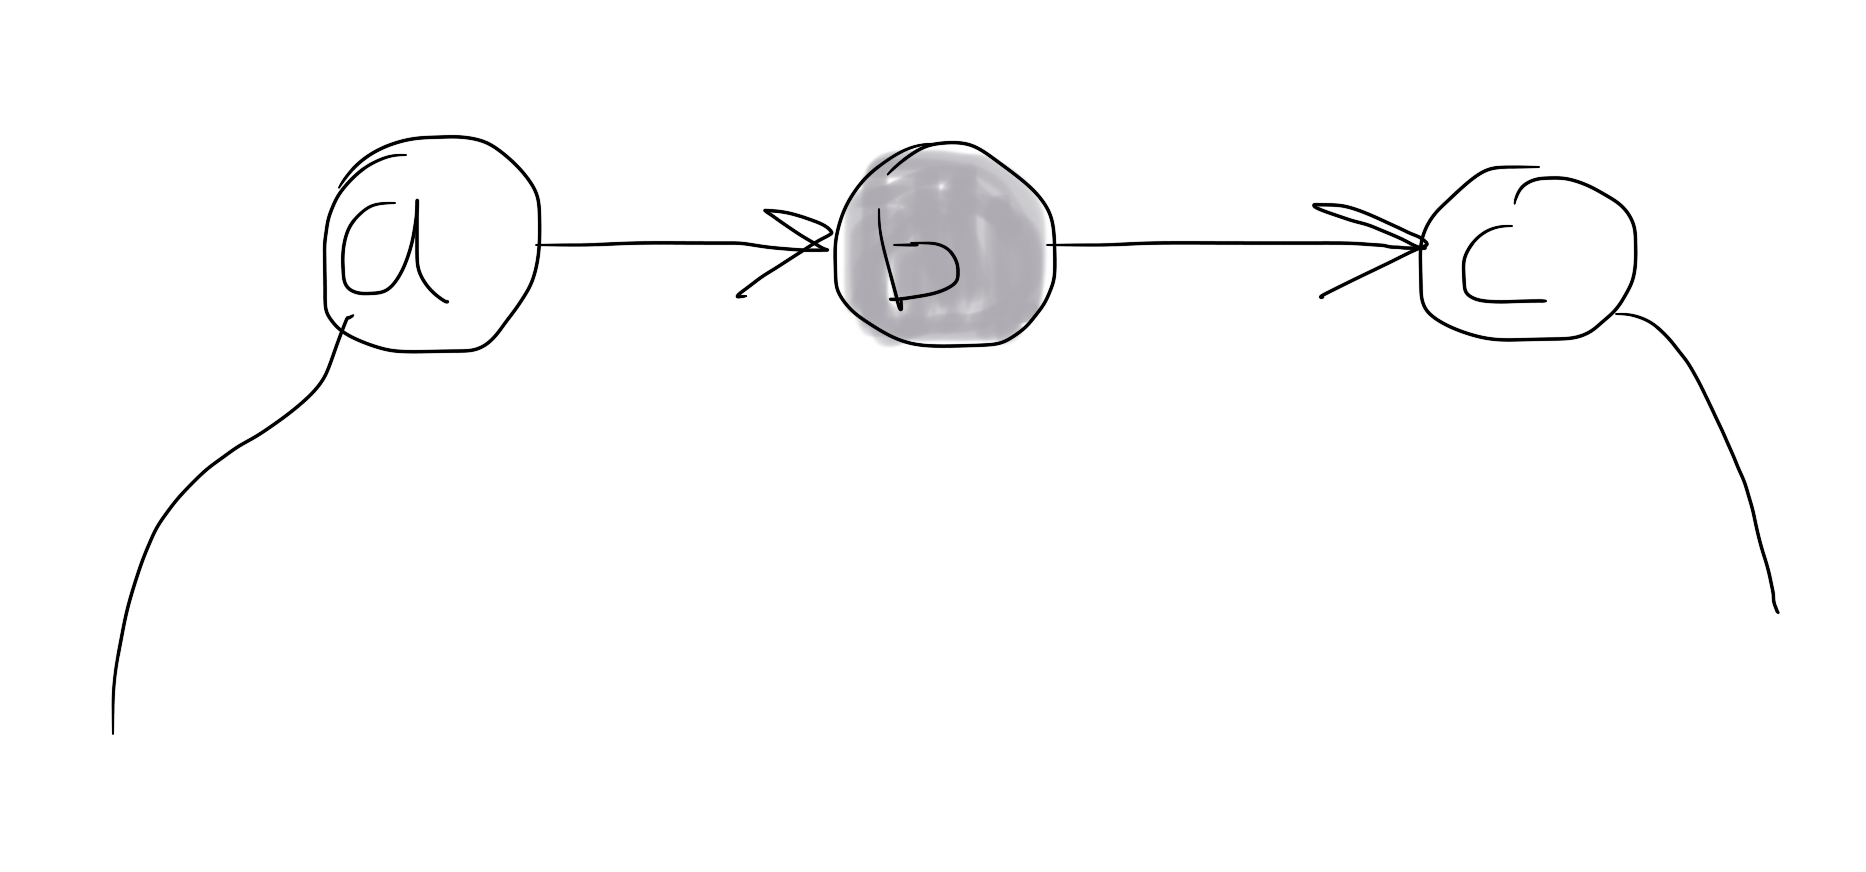
\includegraphics[scale=0.07]{imgs/img4.png}
			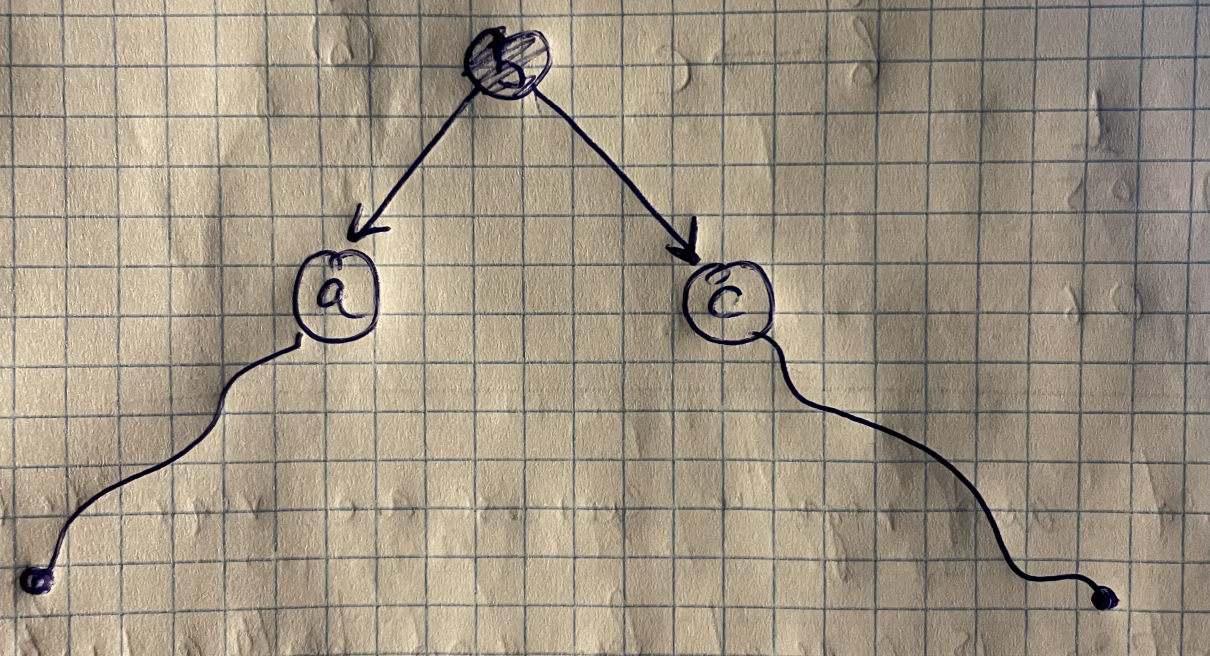
\includegraphics[scale=0.07]{imgs/img5.png}
			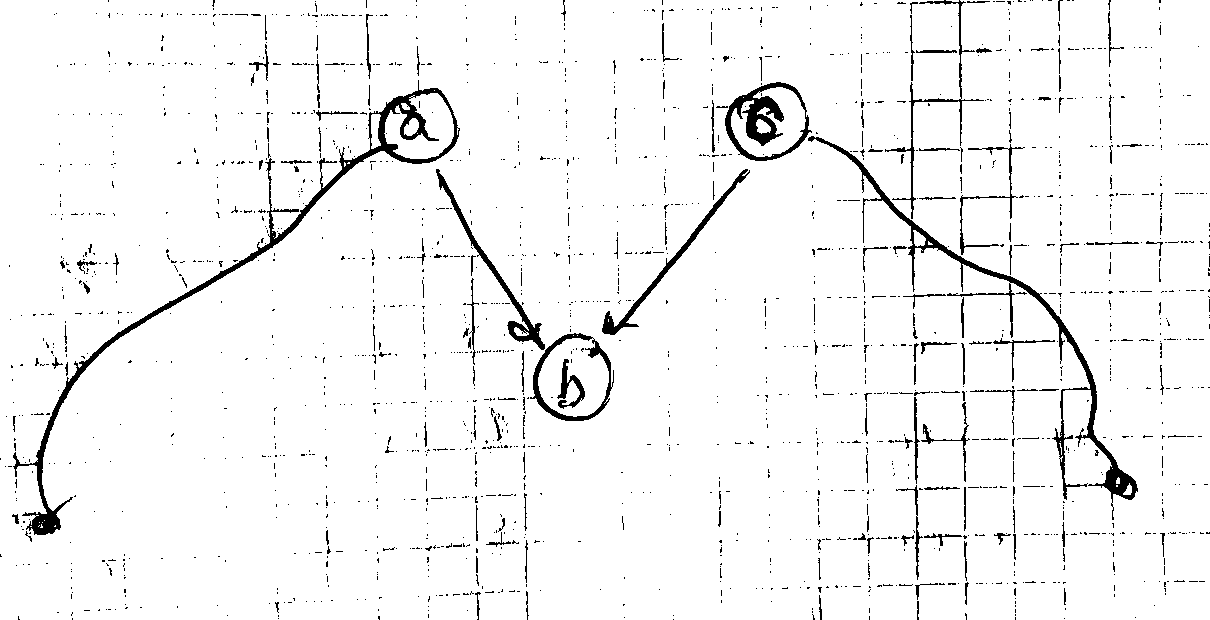
\includegraphics[scale=0.08]{imgs/img6.png}
		\end{center}
		\caption{Various cases of $d$-separation, shaded vertices $\in Z$}
		\label{fig:dsep1}
	\end{figure}
	
	A set $Z$ $d$-separates sets $X$ and $Y$ if it blocks all paths between $X$ and $Y$.
	
	\subsection*{Applications of $d$-separation}
	
	Why did we introduce $d$-separation? Here's why:
	
	\begin{theorem} Probabilistic consequences of $d$-separation\\
		If sets $X$ and $Y$ are $d$-separated by set $Z$, then $X \independent Y\ |\ Z$ in any distribution compatible with $G$. Conversely, if $X$ and $Y$ are not $d$-separated by $Z$ in $G$, then there exists at least one compatible distribution where $X \not \independent Y \ | \ Z$.
		\label{th:th1}
	\end{theorem}
	
	Proof: We begin by introducing the concept of a semi-graphoid relation.
	
	\vspace{0.2cm}
	
	\define{Dependency model} is a ternary relation over subsets of $2^V$ of some set $V$, where triples are interpreted as independence statements between the first and third elements given the second.
	
	\define{Semi-graphoid} is the closure of a dependency model under the first four properties ($X, Y, Z, W$ are disjoint subsets of the carrier set $V$):
	\begin{tcolorbox}
		1. Symmetry: $I(X, Z, Y) \iff I(Y, Z, X)$ \\
		2. Decomposition: $I(X, Z, Y\cup W) \implies I(X, Z, Y)\ \&\ I(X, Z, W)$\\
		3. Weak union: $I(X, Z, Y\cup W) \implies I(X, Z \cup W, Y)$\\
		4. Contraction: $I(X, Z\cup Y, W)\ \&\ I(X, Z, Y) \implies I(X, Z, Y\cup W)$\\
		5. Intersection: $I(X, Z\cup Y, W)\ \&\ I(X, Z\cup W, Y) \implies I(X, Z, Y\cup W)$
	\end{tcolorbox}
	
If, in addition, the semi-graphoid is closed under the fifth property, it is called a \textbf{graphoid}.

An example of a semi-graphoid (and indeed, why they are interesting in this context), defined on the set of subsets of random variables \( V \), is the relation of conditional independence: \( I(X,Y,Z) \iff X \independent Y\ |\ Z \). If the distribution is also strictly positive, meaning that for any set of variable values \((x_1, \ldots, x_N)\): \(\forall i \in [1..N]\ \sum_{X_j, j \neq i} P(x_1, \ldots, x_N) > 0 \implies P(x_1, \ldots, x_N) > 0\), then the conditional independence relation will be a graphoid. Why is this condition important? Let's consider this when we prove property 5.

\vspace{0.2cm}

Let's prove this to warm up.

1. Symmetry is quite obvious: indeed, if \( P(X, Y | Z) = P(X | Z)P(Y|Z) \), then the symmetric statement is also true, since \( P(Y, X|Z) = P(X, Y|Z) = P(X|Z)P(Y|Z) = P(Y|Z)P(X|Z) \).

2. Decomposition: Let \( P(X, YW | Z) = P(X|Z)P(YW|Z) \). Then, simply sum the left and right sides over the set of values \( W \):

For the left side, we have \(\sum_{w} P(X, YW|Z) = P(X, Y|Z)\).

For the right side, similarly:

\begin{align}
	\sum_{w} P(X|Z)P(YW|Z) = P(X|Z)\sum_{w} P(YW|Z) = P(X|Z)P(Y|Z)
\end{align}

The penultimate transition holds because \( Z \cap W = \emptyset \).

By assumption, the left and right sides are equal, so \( P(X, Y|Z) = P(X|Z)P(Y|Z) \).

3. Weak Union: Let \( P(X, YW|Z) = P(X|Z)P(YW|Z) \). Then, by the decomposition property:

\begin{align}
	P(X, W|Z) = P(X|Z)P(W|Z)
\end{align}

Write the factorization:

\begin{align}
	P(X, Y, Z, W) = P(X, YW|Z)P(Z) = P(X|Z)P(YW|Z)P(Z) = P(X|Z)P(Y|ZW)P(W|Z)P(Z)
\end{align}

\begin{align}
	\begin{split}
		P(X, Y|ZW) &= \frac{P(X, Y, Z, W)}{P(Z, W)} = \frac{P(X|Z)P(Y|ZW)P(W|Z)P(Z)}{P(ZW)} = \frac{P(X, W|Z)P(Y|ZW)P(Z)}{P(ZW)} \\
		&= \frac{P(X, Z, W)P(Y|ZW)}{P(ZW)} = P(X|ZW)P(Y|ZW)
	\end{split}
\end{align}

4. Contraction: Let

\begin{align}
	P(X, W|ZY) &= P(X|ZY)P(W|ZY)\\
	P(X, Y|Z) &= P(X|Z)P(Y|Z)
\end{align}

Consider \( P(X, YW|Z) \):

\begin{align}
	\begin{split}
		P(X, YW|Z) &= \frac{P(X, Y, Z, W)}{P(Z)} = \frac{P(X, W|ZY)P(ZY)}{P(Z)} = \frac{P(X|ZY)P(W|ZY)P(ZY)}{P(Z)}\\
		&= P(X|ZY)P(W|ZY)P(Y|Z) = P(X|ZY)P(Y, W|Z) = \frac{P(X, Y|Z)}{P(Y|Z)}P(Y, W|Z) \\
		&= \frac{P(X|Z)P(Y|Z)}{P(Y|Z)}P(Y, W|Z) = P(X|Z)P(YW|Z)
	\end{split}
\end{align}

5. Intersection: Let

\begin{align}
	P(X, W|Z, Y) &= P(X|Z, Y)P(W|Z, Y)\\
	P(X, Y|Z, W) &= P(X|Z, W)P(Y|Z, W)
\end{align}

Multiply the first identity by \( P(Y) \) and the second by \( P(W) \):

\begin{align}
	P(X, W, Y|Z) &= P(X|Z, Y)P(W|Z, Y) P(Y) = P(X|Z, Y)P(W, Y|Z)\label{eq:fifth}\\
	P(X, Y, W|Z) &= P(X|Z, W)P(Y|Z, W) P(Y) = P(X|Z, W)P(Y, W|Z)
\end{align}

Equating the right-hand sides and using the positivity property (this is where it is needed), we cancel \( P(Y, W|Z) \) and obtain:

\begin{align}
	P(X|Z, Y) = P(X|Z, W)
\end{align}

We see that the right-hand side does not depend on \( Y \), so the left-hand side should not depend on it either: \( P(X|Z, Y) = P(X|Z) \). Similarly, \( P(X|Z, W) = P(X|Z) \).

What we need to show is that \( P(X, Y, W|Z) = P(X|Z)P(Y, W|Z) \). It can be noticed that this follows from \ref{eq:fifth} if we use the independence \( X \independent Y\ | \ Z \) derived earlier.

Well, in general, everything seems correct :) More interestingly, these properties are sufficient to define all properties of probabilistic independence.

Now let's move on to how to define a dependency model on a given set. Clearly, one naive approach is to define it explicitly by enumerating a list of triples \((X, Z, Y)\) for which the independence relation holds. However, this list will generally grow exponentially with the size of the carrier set, as the number of its subsets grows exponentially. Representing the dependency model as a graph, on the other hand, can be intuitive, compact, and graphs can be efficiently processed.

There are, as usual, two main options: to use \textbf{undirected} and \textbf{directed} graphs.

In the case of \textbf{undirected} graphs, the interpretation is quite simple: elements of the set are assigned to vertices, and sets of vertices \( X \) and \( Y \) are independent given \( Z \) if \( Z \) separates \( X \) and \( Y \) in the usual sense of graph theory, i.e., if any path from \( X \) to \( Y \) necessarily contains at least one vertex from \( Z \).

It should be noted that not every semi-graphoid can be exactly represented in this form: in most cases, the graph will lack some independences. For example, if the dependency model over a set of three elements \( V = \{x, y, z\} \) contains only the single independence \( I(\{x\}, \{y\}, \emptyset) \), then the corresponding semi-graphoid (note: in the semi-graphoid, there will be two independences due to symmetry) cannot be represented without adding extra dependencies or removing existing independences.

In fact, the set of semi-graphoids that are exactly representable by undirected graphs is the closure of a much stronger class of properties:

\begin{tcolorbox}
	1. Symmetry: \( I(X, Z, Y) \iff I(Y, Z, X) \) \\
	2. Decomposition: \( I(X, Z, Y \cup W) \implies I(X, Z, Y)\ \&\ I(X, Z, W) \) \\
	3. \textbf{Strong} union: \( I(X, Z, Y) \implies I(X, Z \cup W, Y) \) \\
	4. Intersection: \( I(X, Z \cup Y, W)\ \&\ I(X, Z \cup W, Y) \implies I(X, Z, Y \cup W) \) \\
	5. Transitivity: \( I(X, Z, Y) \implies I(X, Z, W) \lor I(Y, Z, W)\ \forall \ W:\ W \cap (X \cup Y \cup Z) = \emptyset \)
\end{tcolorbox}

Well, it's quite clear that these properties hold for representations as undirected graphs. Let's prove that a relation closed under these properties is a graphoid. Essentially, three of the graphoid properties coincide in this definition, so we only need to derive the remaining two: weak union and contraction.

Let's start with weak union: \( I(X, Z, Y \cup W) \implies I(X, Z, Y) \implies I(X, Z \cup W, Y) \), where the first transition is due to the decomposition property, and the second is due to the strong union property.

Let's prove the contraction property: \( I(X, Z, Y) \implies I(X, Z \cup W, Y) \) by the strong union property, so \( I(X, Z \cup Y, W)\ \&\ I(X, Z, Y) \implies I(X, Z \cup Y, W)\ \&\ I(X, Z \cup W, Y) \implies I(X, Z, Y \cup W) \), where the last transition is made by the intersection property.

\vspace{0.2cm}

So, it's clear that undirected graphs are cool, but they can represent a rather limited subset of possible dependency models (here and below, we will use this term as a synonym for semi-graphoid, assuming that the dependency model is closed under properties 1-4 of the semi-graphoid).

Generally speaking, we often don't need a perfect representation of the dependency model, but rather a reasonable approximation that does not contain \textbf{all} the independences defined by the model but at least does not contain extra ones. Such a representation is called an \textit{I-map} (from \textit{independence}).

Let's move on to representing the dependency model as directed graphs, or more precisely, DAGs. The interpretation of such graphs is simple: an edge means a direct causal dependence between two variables. Alas, simple cuts of the graph in this case will no longer reflect independence, since conditioning on some common consequence of two unrelated events can make them dependent. Therefore, instead of ordinary graph separation, the concept of d-separation is introduced (we've already talked about it).

\define{Tail boundary} of a variable \( x \) is a subset \( B \) of the set of variables \( L \) less than \( x \) in the sense of some total order on the set of variables such that \( I(x, B, L \backslash B) \).

\define{Stratification protocol} \( L_\theta = (\theta, B(x)) \) is a pair consisting of a total ordering of variables \( \theta \) and a function \( B(x) \) mapping a variable to its tail boundary.

A DAG is uniquely constructed from the stratification protocol in an obvious way. Clearly, for a given dependency model on \( n \) variables, there are \( n! \) total orderings. For each total ordering, in the worst case, there are \( 2^{n(n-1)/2} \) different ways to define the tail boundaries (for each variable, all previous ones in the worst case can either be present in the boundary or not \(\implies\) for the \( i \)-th variable, there can be \( 2^{i-1} \) different functions defining the tail boundary). Thus, there can be up to \( n!2^{\frac{n(n-1)}{2}} \) different stratification protocols for a given dependency model.

It is claimed that if the dependency model has a perfect representation as a DAG (i.e., there exists a DAG in which all the independences from the model are present, and only they, or equivalently, it is both an I-map and a D-map simultaneously), then one of the stratification protocols defines it. Let's prove this.

Consider the graph \( D \) that perfectly represents the model. It defines a partial order on the set of variables \( \phi \). Let \( \theta \) be any total order consistent with \( \phi \). Then \( L = (\theta, Par(x)) \) will define a stratification protocol generating \( D \) (it's easy to see that the immediate parents of \( x \) are the tail boundary).

\(\blacksquare\)

If there exists a perfect representation of the model as a DAG, then it can be found; however, checking for its existence is generally a complex task. In practice, it is often sufficient to find a minimal I-map, and the following theorem will show that for any semi-graphoid (not necessarily having a perfect representation as a DAG), stratification protocols can be used to construct an I-map.

\begin{theorem} If \( M \) is a semi-graphoid, and \( L_\theta \) is any of its stratification protocols, then the DAG generated by this protocol will be an I-map of the semi-graphoid.
\end{theorem}

Proof by induction on the number of variables in the model. Clearly, for a model with one variable, there is a unique DAG, and it is certainly an I-map. Now suppose the statement is true for models with fewer than \( k \) variables. Let \( M \) have \( k \) variables, and let \( L_\theta \) be its stratification protocol, with the last variable in order \( \theta \) being \( n \), \( M-n \) the semi-graphoid obtained by removing all independence relations containing the variable \( n \), \( G-n \) the DAG with the vertex \( n \) and all edges incident to it removed. Since \( n \) is the last variable in the ordering, it is not contained in any tail boundary in the protocol \( L_\theta \), so \( L_\theta - n \) (this is \( L_\theta \) with the rule for variable \( n \) removed) will be a stratification protocol for \( M-n \). The graph generated by \( L_\theta - n \) will be \( G-n \), and by induction, it is an I-map of \( M-n \).

Let \( M_G \) be the dependency model constructed from \( G \) (i.e., using all possible d-separations in the graph), \( M_{G-n} \) be the model generated from \( G-n \). Side note: in principle, \( M_G \) can contain more independences than there are d-separations in \( G \), as it is built as the closure of all independences obtained from \( G \), but it seems we need to prove that there are no extra independences (this will be addressed by the lemma below). By induction, as mentioned above, \( M_{G-n} \subset M-n \). Accordingly, we need to show that \( M_{G} \subset M \). Any triple \( T \in M_G \) can be classified into one of four disjoint categories: either \( n \) is not represented in any of the three sets composing \( T \), or \( n \) is in one of these three sets.

\textbf{Lemma} Let \( G \) be a DAG, and \( M_G \) be the dependency model induced by it. Then \( G \) is a perfect representation of \( M_G \) as a DAG.
Note that \( G \) is an I-map for \( M_G \), since all independences from \( G \) are present in \( M_G \) by construction. Thus, it remains to show that \( G \) is a D-map. For this, we need to prove that properties 1-4 of the semi-graphoid hold in \( G \) (since then the d-separated triples are closed in \( G \), and hence in \( M_G \)).

1. The symmetry property obviously holds (if \( X \indepg Y \ | \ Z \implies Y \indepg X \ | \ Z \)).

2. The decomposition property is also obviously true: if \( Z \) blocks the paths between \( X \) and \( Y \cup W \), then \( Z \) certainly blocks the paths between \( X \) and \( Y \).

3. The weak union property: let \( X \indepg Y \cup W | Z \). We need to show that \( X \indepg Y | Z \cup W \). We will argue by contradiction: suppose not. Note that by the decomposition property, \( X \indepg Y | Z \) and \( X \indepg W | Z \). Thus, adding \( W \) to \( Z \) unblocked some path between \( X \) and \( Y \). But this is only possible if the unblocked path \( X \leadsto Y \) has a v-structure with an endpoint in \( W \), i.e., \( X \leadsto \ldots \rightarrow w \leftarrow \ldots \leadsto Y \), where \( w \in W \). Clearly, in this case, the path \( X \leadsto w \) is unblocked. Consider this path similarly (it will be shorter than the previous one). It was either unblocked before conditioning on \( W \), or became so after. In the second case, we repeat the logic and again truncate the path, repeating the approach until we arrive at the first case. In the first case, the prefix of the path up to \( w \) is unblocked when conditioning on \( Z \), but then \( X \not \indepg w | Z \), which contradicts the initial assumption.

4. Finally, the contraction property. Let \( X \indepg W | Z \cup Y \) and \( X \indepg Y | Z \). We need to show that \( X \indepg Y \cup W | Z \).

Well, let's start with the fact that by condition, \( Z \) blocks all paths \( X \leadsto Y \). Thus, it remains to show that \( Z \) blocks all paths \( X \leadsto W \). Suppose not. Then there exists an unblocked path \( p = X \leadsto W \). Note that by condition, \( Z \cup Y \) separates \( W \) from \( X \), so \( Y \) must block the path \( p \), and hence \( p = X \leadsto \ldots \rightarrow y \rightarrow \ldots W \) or \( p = X \leadsto \ldots \leftarrow y \rightarrow \ldots \leadsto W \), where \( y \in Y \), and the prefix of the path \( p \) up to \( y \) is not blocked by \( Z \) (otherwise the path would be blocked without conditioning on \( y \)). But this in turn means that there exists an unblocked path from \( X \) to \( y \), which contradicts the fact that \( Z \) d-separates \( X \) and \( Y \).

\(\blacksquare\)

Thus, it is now shown that \( (X, Z, Y) \in M_G \iff X \indepg Y | Z \), i.e., the d-separation relation defines a graphoid on the DAG.

\textbf{Case 1}: \( n \) is not represented in \( T = (X, Z, Y) \). \( T \in M_G \implies T \in M_{G-n} \), since otherwise there would be an unblocked path in \( G-n \) not blocked by \( Z \), but then the same unblocked path exists in \( G \), since adding vertices and edges cannot block a path. \( G-n \) is an I-map for \( M-n \), so \( T \in M-n \), and since \( M-n \subset M \), then \( T \in M \).

\textbf{Case 2}: \( T = (X, n, Z, Y) \). Let \( (n, B, R) \in L_\theta \) be the last triplet of the stratification protocol (and of course the only one containing \( n \)), \( B = B_X \cup B_Y \cup B_Z \cup B_0 \), \( R = R_X \cup R_Y \cup R_Z \cup R_0 \), where \( X = B_X \cup R_X \), \( Y = B_Y \cup R_Y \), \( Z = B_Z \cup R_Z \) \ref{fig:case2}.

\begin{figure}[h]
	\begin{center}
		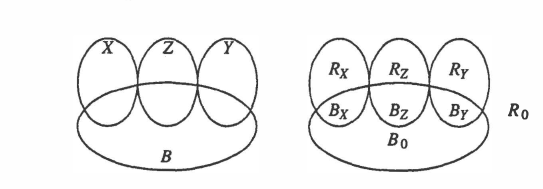
\includegraphics[scale=0.6]{imgs/img7.png}
	\end{center}
	\caption{Case 2}
	\label{fig:case2}
\end{figure}

By construction, there is an edge from all vertices \( B \) to \( n \). Since \( T \in M_G \), any path between \( n \) and \( Y \) must be blocked by \( Z \), so \( B_Y = \emptyset \), otherwise there would be a path consisting of just one edge from \( b \in B_Y \) to \( n \). Thus, \( Y = R_Y \), and the last triplet of the protocol can be represented as \( (n, B_X B_0 B_Z, R_X R_Z R_0 Y) \).

Since \( M \) is a semi-graphoid, by the weak union property, we can move \( R_X R_Z \) from the third element of the triplet to the second and obtain a valid independence relation: \( (n, B R B_0, Y R_0) \in M \). Also, by decomposition, we can ignore \( R_0 \) in the last element of the triplet and again obtain an element of \( M \):

\begin{align}
	(n, X Z B_0, Y) \in M
	\label{eq:case2}
\end{align}

All elements \( B_0 \) are connected by an edge to \( n \), and \( n \) is d-separated from \( Y \) by the vertices \( Z \), so \( B_0 \) is also d-separated from \( Y \) by the same \( Z \), since otherwise there would be a path \( B_0 \leadsto Y \), but then, because \( B_0 \rightarrow n \), there would be an unblocked path \( Y \leadsto n \) not blocked by \( Z \). Now, since \( X \) and \( B_0 \) are d-separated from \( Y \) via \( Z \), their union is also separated from \( X \) via \( Z \), so \( (X B_0, Z, Y) \in M_G \). In this triplet, \( n \) does not appear, so by case 1, we have \( (X B_0, Z, Y) \in M \). Combining this with \ref{eq:case2} and using the contraction property, we obtain \( (Y, Z, n X B_0) \in M \), and then by the decomposition property, \( (n X, Z, Y) \in M \).

\textbf{Case 3}: \( T = (X, n Z, Y) \). Again, represent the last element of the stratification protocol as \( (n, B_X B_Y B_Z B_0, R_X R_Y R_Z R_0) \in M \). Note that \( B_X = \emptyset \lor B_Y = \emptyset \), since otherwise there would be a path \( b_x \rightarrow n \leftarrow b_y \), unblocked by conditioning on \( n \), i.e., there would be an unblocked path \( X \leadsto Y \), which would contradict \( T \in M_G \). Without loss of generality, let \( B_Y = \emptyset \). By considerations from the previous point, \( (B_0, Z, Y) \in M_G \).

Further, \( (X, n Z, Y) \in M_G \implies (X, Z, Y) \in M_G \), since \( n \) has only incoming edges, so if there were an unblocked path \( X \leadsto Y \) not blocked by \( Z \), conditioning on \( n \) would not help block it. Thus, \( (X B_0, Z, Y) \in M_G \), and by case 1, also \( (X B_0, Z, Y) \in M \). By reasoning from case 2, the last triplet of the protocol can be represented as \( (n, B_X B_0 B_Z, R_X R_Z R_0 Y) \in M \) and ultimately \( (n, X Z B_0, Y) \in M \implies (n X B_0, Z, Y) \in M \implies (X B_0, n Z, Y) \implies (X, n Z, Y) \) (weak union, then decomposition).

\textbf{Case 4}: \( T = (X, Z, n Y) \) - by symmetry, reduces to case 2.

\(\blacksquare\)

\begin{tcolorbox}
	In essence, how to use this theorem, that is, what are the implications? Here they are: suppose there is a dependency model (any semi-graphoid), and we have constructed some stratification protocol \( L_\theta \) for it, and from the stratification protocol, we have constructed a DAG. So, any d-separation of sets in the DAG means the membership of the corresponding triple (conditional independence) in the dependency model.
\end{tcolorbox}

Another simple corollary: if the stratification protocol \( L_\theta \) of the dependency model \( M \) is such that all tail boundaries in it are minimal (no element can be removed from any of them without violating the membership of the triplet in \( M \)), then the DAG constructed from this protocol is a minimal I-map of the model—obviously, it is an I-map by the theorem, and minimal because each edge is determined by some tail boundary of the protocol, meaning no edge can be removed without violating the I-map (otherwise, we would reconstruct from the truncated DAG back to the truncated stratification protocol, and it would be correct).

Returning to the original theorem about the consequences of d-separation in the context of probability distributions: we have shown that if \( P(V) \) is Markov relative to the DAG \( G \), then \( X \indepg Y | Z \implies X \independent Y | Z \). Well, because in this case, \( P(V) \) acts as a dependency model, and Markov compatibility allows constructing a stratification protocol of this model corresponding to \( G \). But nothing has been done yet with the second statement of the theorem: that if in the graph there is no d-separation of sets \( X, Y \) by set \( Z \), then there exists a distribution compatible with \( G \) in which \( X \not\independent Y | Z \). For now, let's leave this fact unproven.

\begin{theorem} \textbf{Ordered Markov Condition}\\
	A necessary and sufficient condition for the distribution \( P \) to be Markov compatible with \( G \) is that each variable is independent of all its predecessors in some ordering consistent with \( G \) when conditioned on its parents in \( G \).
	\label{th:ordered_markov}
\end{theorem}

\textbf{Necessity}: Let \( P \) be compatible with \( G \). This means that \( P(x_1..x_n) = \prod P(x_i|pa_i) \). Order the variables using topological sorting according to the graph \( G \). We need to show that \( P(x_i | pa_i, x_j) = P(x_i | pa_i) \).

Note that

\begin{align}
	P(x_1...x_n) = \prod\limits_{k\le i}P(x_k|pa_k)\prod\limits_{k> i} P(x_k | pa_k)
	\label{eq:factorization1}
\end{align}

From this, the marginal distribution of the first \( i \) variables in our chosen order is easily derived by summing the equality

\begin{align}
	\begin{split}
		P(x_1...x_i) &= \prod\limits_{k\le i}P(x_k|pa_k)\sum\limits_{x_j: j > i}\prod\limits_{k> i} P(x_k | pa_k)\\
		&= \prod\limits_{k\le i}P(x_k|pa_k)\sum\limits_{x_j : i < j < n}\prod\limits_{ i < k < n}P(x_k | pa_k) \sum\limits_{x_n}P(x_n | pa_n)\\
		&= \ldots = \prod\limits_{k\le i}P(x_k|pa_k)
		\label{eq:factorization2}
	\end{split}
\end{align}

Using \ref{eq:factorization2}, we easily derive the relation

\begin{align}
	P(x_i|x_1,...,x_{i-1}) = \frac{P(x_1,...,x_i)}{P(x_1,...,x_{i-1})} = \frac{\prod\limits_{k\le i}P(x_k|pa_k)}{\prod\limits_{k\le i - 1}P(x_k|pa_k)} = P(x_i|pa_i)
\end{align}

Thus, \( X_i \independent \{x_1...x_{i-1}\} \backslash PA_i\ |\ PA_i \). We have already proven earlier that the conditional independence relation for a set of random variables forms a graphoid, and therefore, by the decomposition property, \( \forall j < i: X_j \notin PA_i \implies X_i \independent X_j | PA_i \), which is what was required.

\textbf{Sufficiency}: Let each variable \( X_i \) be independent of all variables with a smaller number when conditioned on the immediate ancestors of the variable in the graph \( G \). Let us show that in this case, the distribution is Markov compatible with \( G \), i.e., that it factorizes according to \( G \).

Any distribution can be represented in the following factorization:

\begin{align}
	P(x_1,...,x_n) = \prod\limits_i P(x_i|x_1,...,x_{i-1})
\end{align}

Note that now it remains for us to use the condition that each variable is conditionally independent of all variables with a smaller number when conditioned on its parents in the graph \( G \), to obtain the necessary equality:

\begin{align}
	P(x_1,...,x_n) = \prod\limits_i P(x_i|pa_i)
\end{align}

\(\blacksquare\)

Another similar theorem:

\begin{theorem} \textbf{Parental Markov Condition}\\
	A necessary and sufficient condition for the distribution \( P \) to be Markov compatible with \( G \) is that each variable is independent of all its \textit{non-descendants} in some ordering consistent with \( G \) when conditioned on its parents in \( G \).
\end{theorem}

\textbf{Necessity}: Let \( P(v) \) be compatible with the graph \( G \), and \( x_j \notin de(x_i) \). Let us show that \( x_i \independent x_j \ |pa_i \). Note that if \( j < i \), then the statement follows from the previous theorem on the ordered Markov condition. Let \( j > i \). Clearly, in the graph \( G \), there is no directed path \( x_i \leadsto x_j \) (since \( x_j \notin de(x_i) \)), nor a directed path \( x_j \leadsto x_i \), since in this case, the ordering of the variables would not be consistent with the graph topology. Therefore, in any path connecting \( x_i \) and \( x_j \), there is at least one connection of the form \( \rightarrow x_k \leftarrow \), and of course \( x_k \notin pa_i \), since then there could not be two arrows in the path. But any such path is blocked by the set \( pa_i \), so \( x_i \) and \( x_j \) are d-separated in \( G \) by the set \( pa_i \), and therefore, conditionally independent when conditioned on \( pa_i \) according to the probabilistic consequences of d-separation.

\textbf{Sufficiency}: Here everything is simple: if each variable is independent of its non-descendants, then it is certainly independent of all variables with smaller numbers than its own, and therefore, by the previous theorem, the distribution is compatible with \( G \).

\(\blacksquare\)

\define{Observational Equivalence} Two graphs are called observationally equivalent if any distribution compatible with the first is compatible with the second, and vice versa.

\begin{theorem} \textbf{On Observational Equivalence}\\
	Two graphs are observationally equivalent if and only if they have the same skeleton and set of \( v \)-structures.
\end{theorem}

\textbf{Necessity}: Let two graphs be observationally equivalent. Let us prove that they have the same skeleton and set of v-structures.

Let's start with the skeleton. Suppose the graph \( G_1 \) has an edge \( x-y \), and \( G_2 \) does not. Consider the following distribution:

\begin{align}
	P(x_1,..x_n) = uniform_{[0,1]}(x)bernoulli_x(y)
\end{align}

where all variables except the two under consideration are constant. Note that such a distribution will be compatible with \( G_1 \), as it factorizes according to it. At the same time, it is not compatible with \( G_2 \). Indeed, suppose it is compatible. According to the ordered Markov condition theorem \ref{th:ordered_markov}, in this case, there exists an ordering consistent with \( G_2 \) in which each variable is independent of variables with smaller numbers when conditioned on its parents in \( G_2 \). Without loss of generality, assume that \( x \) is ordered before \( y \). Note that \( x \notin PA_y \), since there is no edge between them in \( G_2 \), so \( P(y|x) = \sum_{pa_y} P(y, pa_y|x) = \sum_{pa_y} P(y|x, pa_y) P(pa_y|x) = \sum_{pa_y} P(y|pa_y) = P(y) \), i.e., \( y \) should be independent of \( x \) in \( P \), but this is not the case. We have arrived at a contradiction, so \( P \) is incompatible with \( G_2 \), but then \( G_1 \) and \( G_2 \) are observationally nonequivalent, which contradicts the initial assumption, so \( G_2 \) also does not have the edge \( x-y \). Thus, the skeletons of the graphs coincide.

Now let's prove that the graphs have the same v-structures. Well, this is quite simple to prove: consider any two such graphs, and assume the statement is false. We already know that the skeletons of the graphs coincide, so the undirected paths also coincide. If the sets of v-structures do not coincide, there is at least one path \( x \leadsto y \), blocked by \( Z \) in the first graph and unblocked in the second (the symmetric case is analogous). Consider this path in both graphs. The difference in blocking can only be due to the different orientation of arrows at some vertex \( v \). There are only four ways to orient arrows in a path:

1. \( ...\rightarrow v \leftarrow ... \), but in this case, \( v \) has the same arrows in both graphs, as it is a vertex of a v-structure, so this vertex cannot distinguish the blocking of the path in the graphs.

2. \( \rightarrow v \rightarrow \)

3. \( \leftarrow v \leftarrow \)

4. \( \leftarrow v \rightarrow \)

The last three options can be observed in both graphs independently. However, in any combination, if \( v \in Z \), then in both graphs \( v \) blocks the path, and if \( v \notin Z \), it does not block. That is, in any case, any valid direction of arrows in \( v \) cannot distinguish the blockedness of the path in the graphs, so the assumption is incorrect.

\textbf{Sufficiency}: Let two graphs have the same skeleton and set of v-structures. We need to show that they are observationally equivalent.

This will require some effort. We will prove by induction on the number of vertices in the graphs. With one vertex, everything is clear and true, so we assume that the base exists.

Suppose we have proved the statement for all graphs with fewer than \( n \) vertices. Consider two graphs on \( n \) vertices with the same skeleton and set of v-structures. Suppose \( P(v) \) is compatible with \( G_1 \), and let us show that it is then also compatible with \( G_2 \).

\begin{figure}[h]
	\begin{center}
		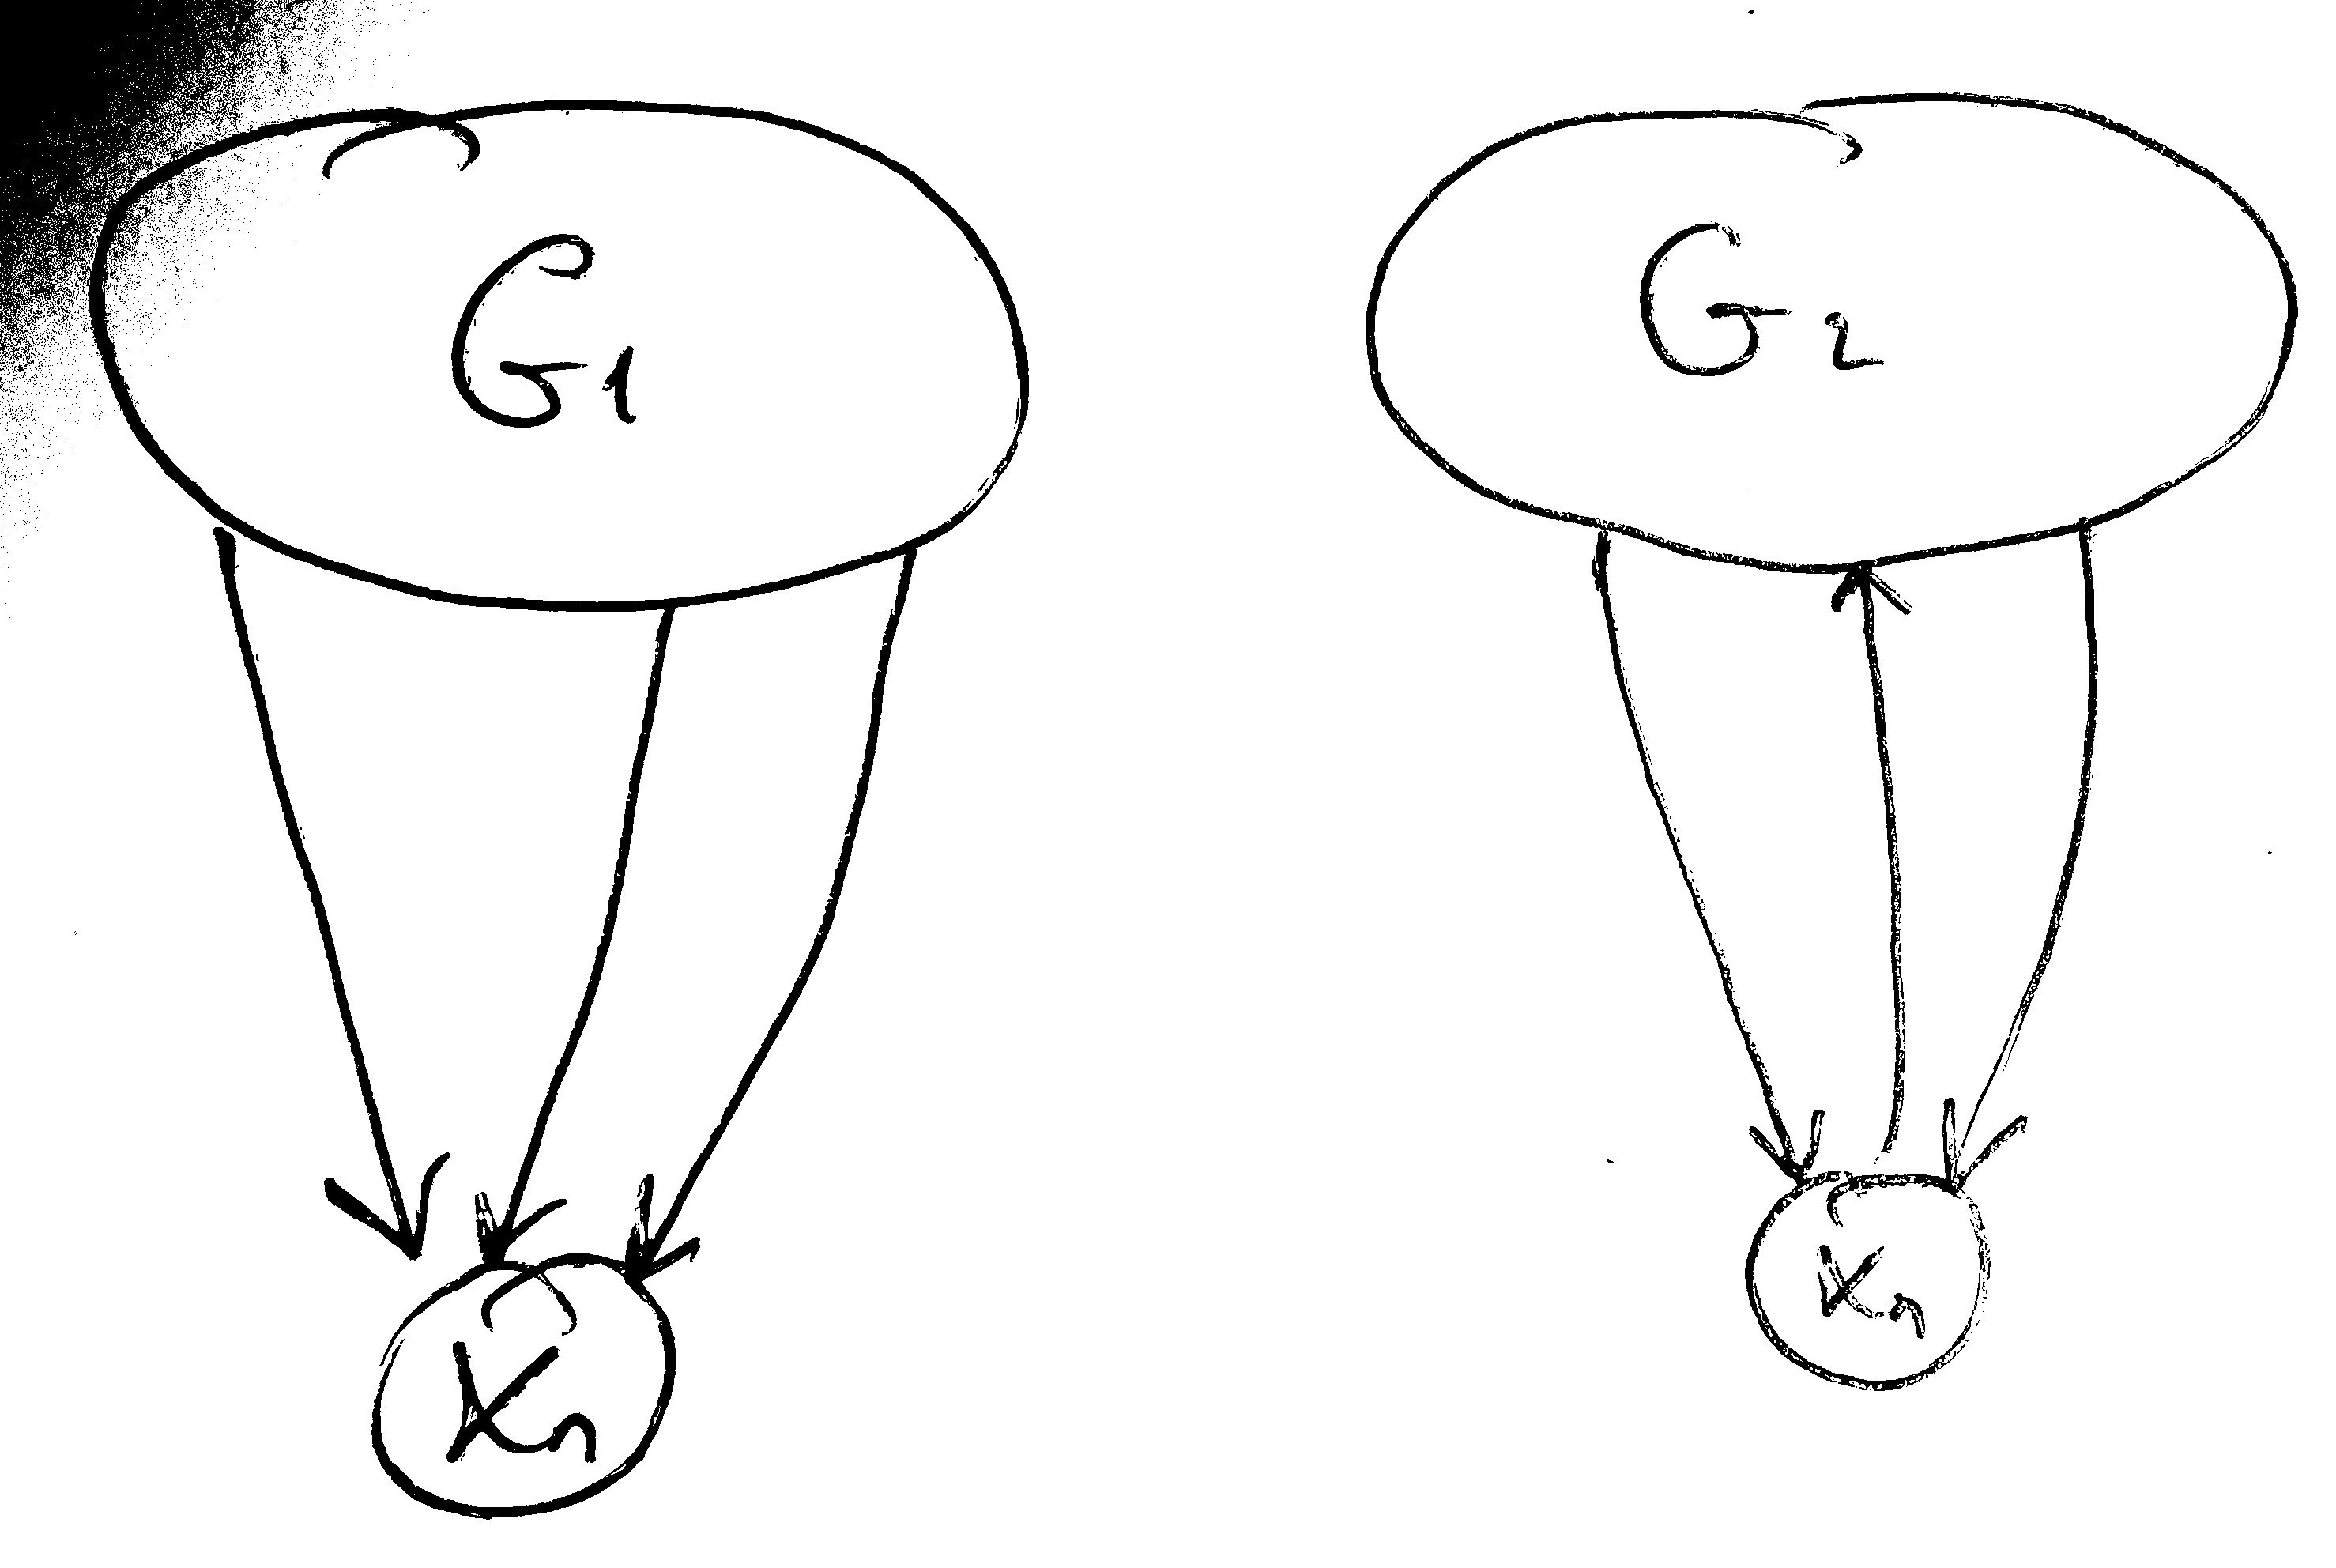
\includegraphics[scale=0.1]{imgs/img10.png}
	\end{center}
	\caption{The two considered graphs \( G_1 \) and \( G_2 \)}
	\label{fig:equiv1}
\end{figure}

Since \( P(v) \) is compatible with \( G_1 \), it factorizes according to it:

\begin{align}
	P(x_1,...x_n) = \prod\limits_{i}P(x_i|pa^1_{i})
\end{align}

We will assume that the variables are ordered according to the topological sorting of graph \( G_1 \), where \( pa^1_i \) represents the parents of node \( X_i \) in \( G_1 \). Similarly, we will denote \( pa^2_i \) as the parents of node \( X_i \) in \( G_2 \). Note that in general, \( pa^1_i \neq pa^2_i \).

Consider the marginal distribution \( P(x_1,...,x_{n-1}) \). It is clearly compatible with \( G_1-x_n \). Furthermore, note that it is also compatible with \( G_2-x_n \), since these two graphs on \( n-1 \) vertices have identical skeletons and v-structures (the skeletons are obvious, and v-structures remain unchanged because we couldn't have created or destroyed any v-structures by removing \( x_n \) from \( G_2 \), just as in \( G_1 \) this variable doesn't participate in forming any v-structures, and similarly in \( G_2 \)). Therefore, we can write:

\begin{align}
	P(x_1,...,x_{n-1}) = \prod\limits_{i}P(x_i|pa^1_{i}) = \prod\limits_{i}P(x_i|pa^2_{i} \backslash \{x_n\}) 
\end{align}

In the last equality, we account for the fact that when removing \( x_n \) from \( G_2 \), some vertices (specifically all those into which \( x_n \) has edges in \( G_2 \)) must have \( x_n \) removed from their parent lists in the graph \( G_2-x_n \).

Now let's return to the full distribution:
\begin{align}
	P(x_1,...x_{n}) = P(x_1,...x_{n-1})P(x_n|pa^1_{n}) = \prod\limits_{i}P(x_i|pa^2_{i} \backslash \{x_n\}) P(x_n|pa^1_{n})
\end{align}

Let's mentally partition the set \( pa^1_n \) into three subsets \( pa^1_n = Q \cup R \cup S \):

\begin{figure}[h]
	\begin{center}
		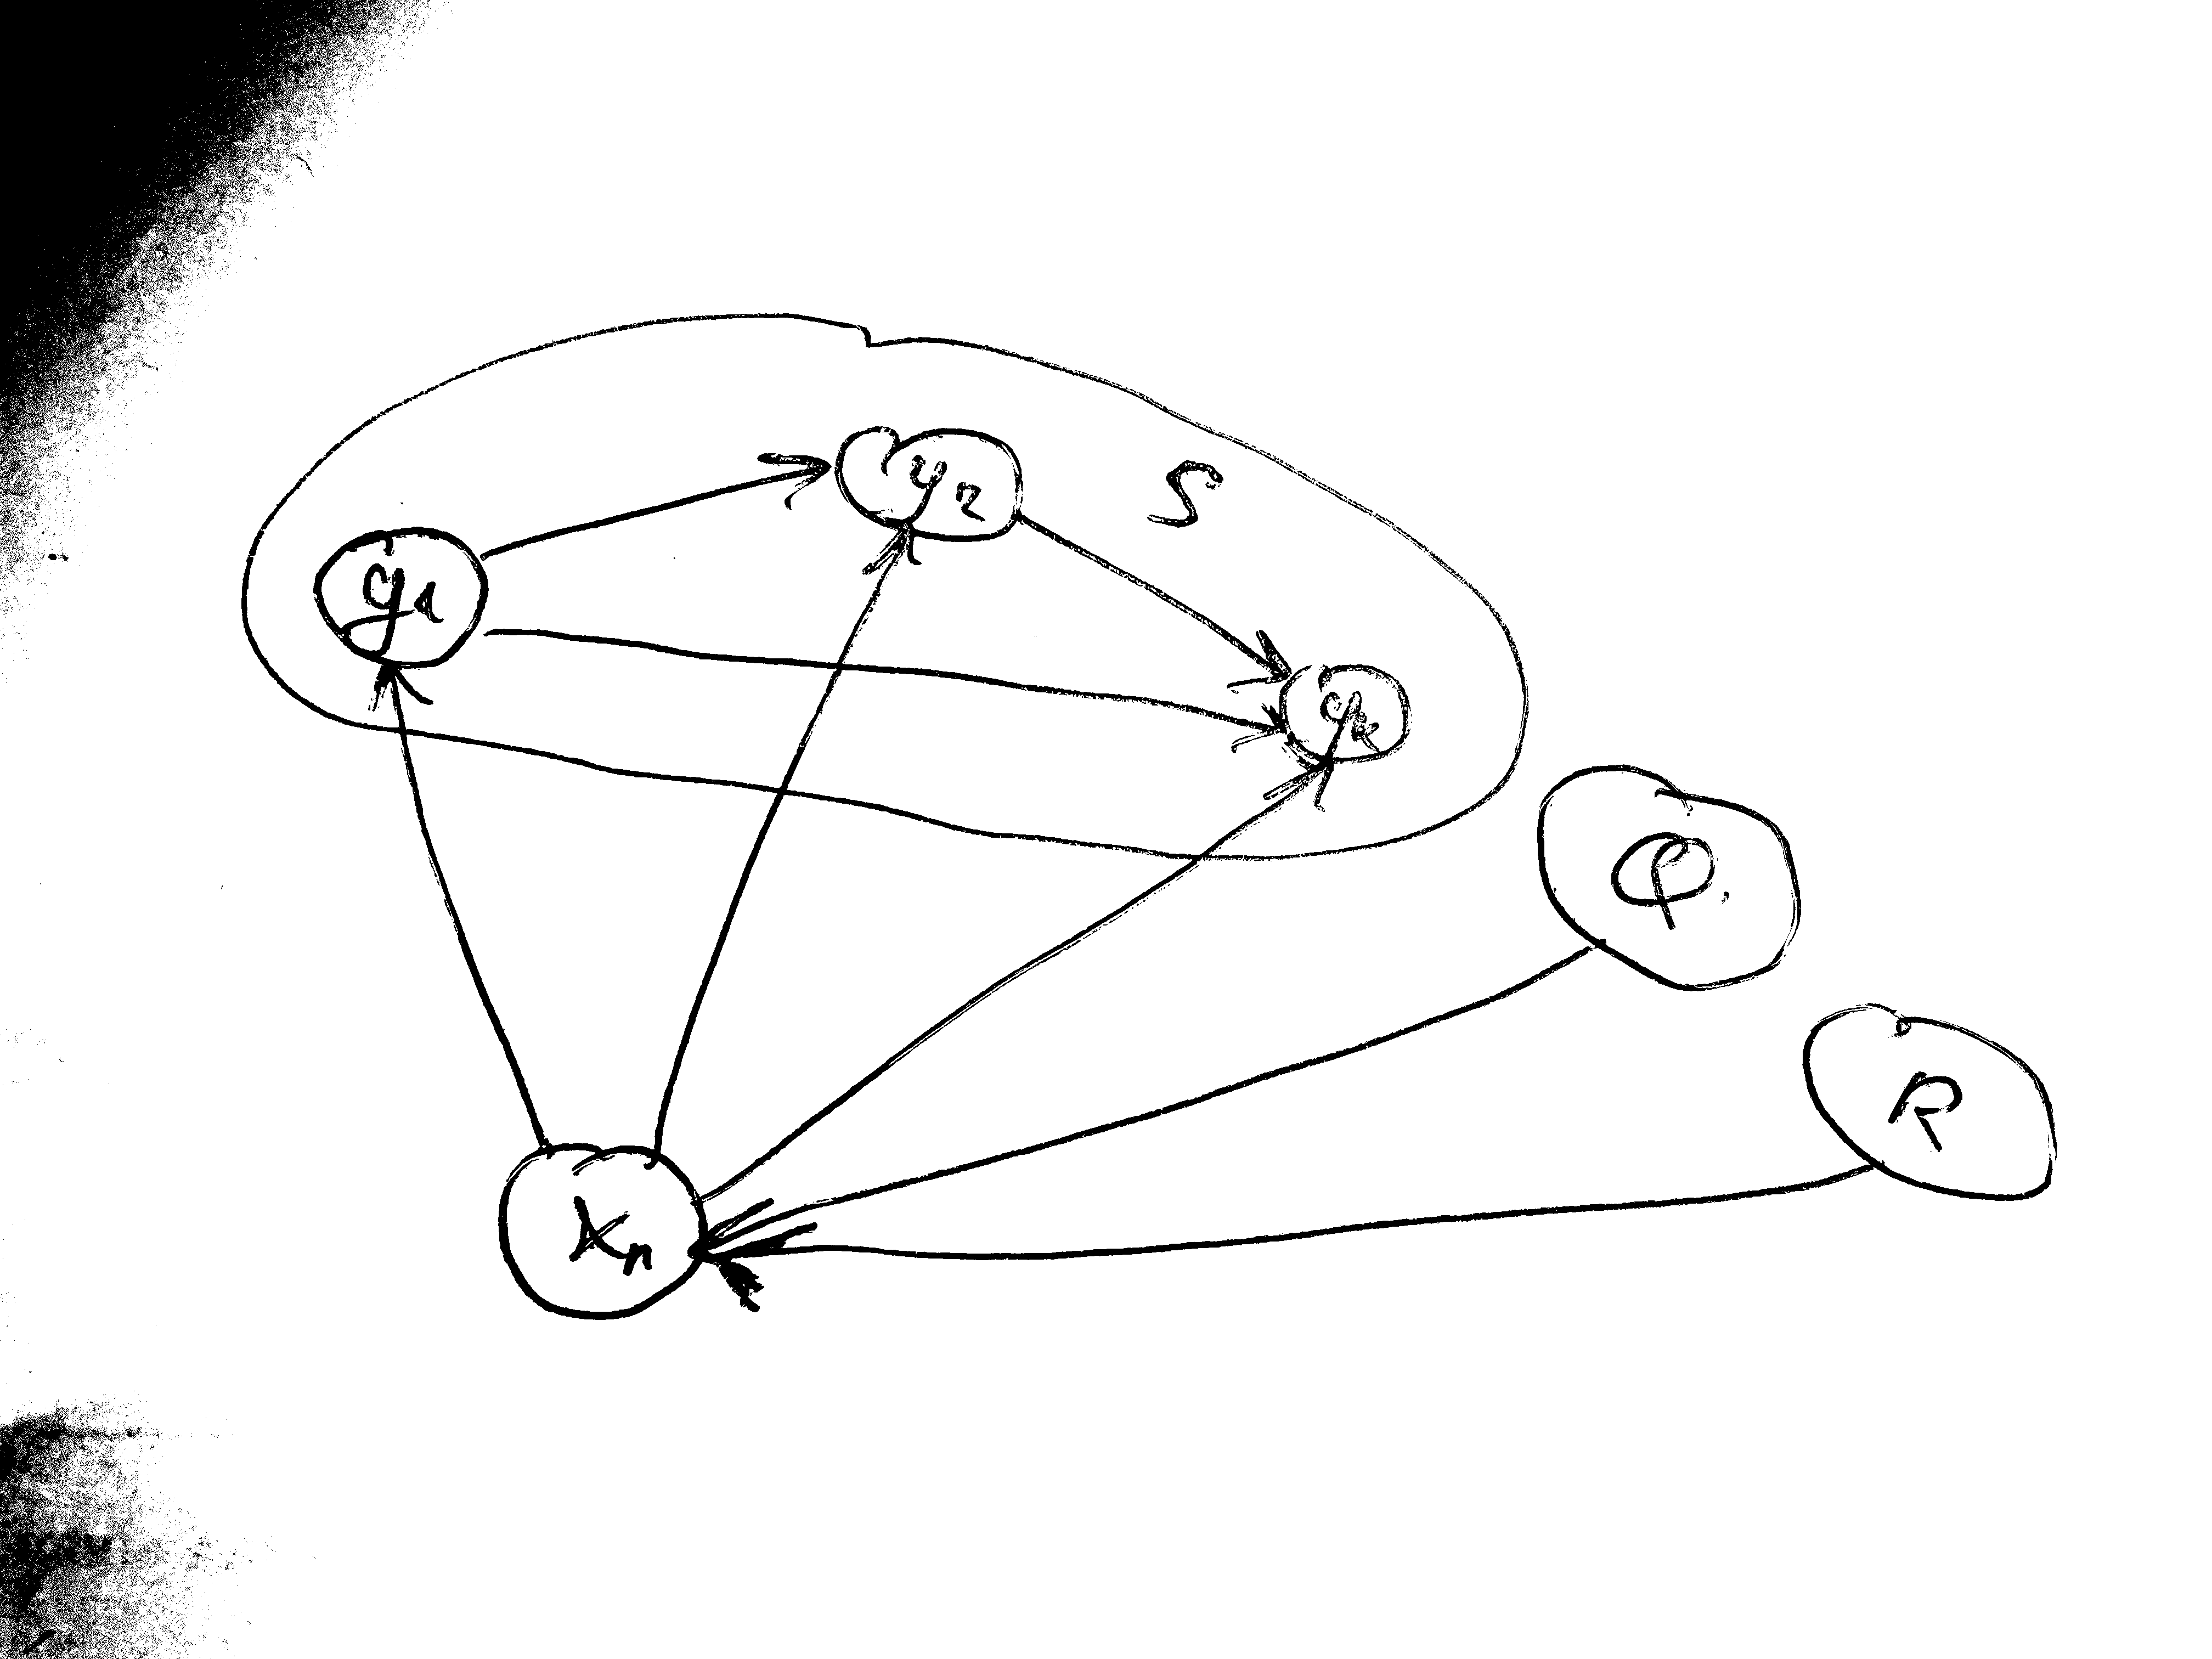
\includegraphics[scale=0.05]{imgs/img11.png}
	\end{center}
	\caption{Partition of variables connected to \( x_n \) into \( Q, R, S \)}
	\label{fig:equiv2}
\end{figure}

Here \( Q \) is the set of vertices forming a v-structure with \( x_n \), i.e., \( x_i, x_j \in Q \iff x_i \rightarrow x_n \leftarrow x_j \) and there is no edge connecting \( x_i \) and \( x_j \). \( R \) is the set of vertices from which there is an edge to \( x_n \) in \( G_2 \). \( S \) is the most interesting set, as it consists of vertices where the edge orientation between them and \( x_n \) is inverted in \( G_2 \) compared to \( G_1 \), meaning these are all vertices for which \( x_n \) is a parent in \( G_2 \). For clarity, see Figure \ref{fig:equiv2}.

Thus, \( pa^1_n = Q \cup R \cup S \), \( pa^2_n = Q \cup R \). Let's focus on set \( S \): we need to understand that these vertices form a clique, meaning they are all interconnected. Indeed, if this weren't the case, there would exist two vertices \( x_i, x_j \in S \): there is an edge from \( x_n \) to them, but they are not connected to each other. But then in \( G_1 \) they would form a v-structure with \( x_n \), which would place them not in \( S \) but in \( Q \). 

We can then represent the factorization of \( P(v) \) as follows:

\begin{align}
	P(x_1,...x_{n}) =  \prod\limits_{x_i\notin S}P(x_i|pa^2_{i})\prod\limits_{x_i\in S}P(x_i|pa^2_{i} \backslash \{x_n\}) P(x_n|Q, R)
	\label{eq:equiv1}
\end{align}

Number the vertices in \( S \) in topological order according to graph \( G_2 \). Clearly, since they are all interconnected, this can be done uniquely. So, let \( S = \{y_1,y_2,...,y_k\} \). 

Note that \( pa^2_{y_j} \subset R \cup Q \cup \{y_1,...y_{j-1}\} \cup \{x_n\} \). Indeed, \( y_{j+1},...y_{k} \) cannot be parents due to our topological numbering. No other vertices \( z \) are present there because if such a vertex existed, there must necessarily be an edge \( z \rightarrow x_n \), otherwise \( x_n \rightarrow y_j \leftarrow z \) would form a v-structure in \( G_2 \) that doesn't exist in \( G_1 \), meaning \( z \in Q \cup R \).

We need to show that \( P(v) = \prod\limits_{i}P(x_i|pa^2_{i}) \). Comparing with \ref{eq:equiv1}, we arrive at the need to show:

\begin{align}
	\prod\limits_{x_i\in S}P(x_i|pa^2_{i} \backslash \{x_n\}) P(x_n|Q, R, S) =  \prod\limits_{x_i \in S}P(x_i|pa^2_{i}) P(x_n|pa^2_n)
	\label{eq:equiv2}
\end{align}

Let's start simplifying the left-hand side, beginning with the factor for \( y_k \) and \( x_n \). Note that \( Q,R \) do not contain descendants of \( y_k \) in \( G_2 - x_n \), otherwise there would be a cycle through \( x_n \). Moreover, \( P(v\backslash \{x_n\}) \) is compatible with \( G_2 - x_n \) by the induction hypothesis. Therefore, according to the parental Markov condition theorem, \( P(y_k | pa^2_{y_k} \backslash \{x_n\}) = P(y_k|y_1,...y_{k-1},Q,R) \).

Then:
\begin{align}
	\begin{split}
		&P(y_k|pa^2_{y_k} \backslash \{x_n\}) P(x_n | Q,R,S) = P(y_k|y_1,...y_{k-1},Q,R) P(x_n | y_1,...y_k,Q,R) \\ 
		&= P(x_n, y_k | y_1,...y_{k-1}, Q, R) \\ 
		&= P(y_{k}|x_n,y_1,...y_{k-1}, Q, R)P(x_n|y_1,...y_{k-1},Q,R) \\ 
		&= P(y_k|pa^2_{y_k})P(x_n|y_1,...y_{k-1},Q,R)
	\end{split}
\end{align}

We can proceed similarly, simplifying the expression for \( y_{k-1}\ldots y_1 \). The result will be exactly what we needed to show in \ref{eq:equiv2}.

$\blacksquare$

Thus, observational equivalence defines the boundaries within which orientation determination in Bayesian networks is possible. To prefer one equivalent Bayesian network over another, we need additional information about the temporal ordering of events, or alternatively, to conduct intervention experiments.

\subsection*{Causal Bayesian Networks}

Strictly speaking, until now we have considered Bayesian networks as a way to represent dependency models generated by probability distributions, where edges in the DAG merely indicated direct dependencies between variables. However, it proves useful to additionally endow edge directions with causal meaning, and accordingly, to construct Bayesian networks such that edge directions reflect causal relationships between variables whenever possible.

The advantage of this approach is modularity - interventions can be made with minimal changes, essentially only affecting edges incident to a particular vertex when that vertex's behavior changes. The benefit is that each directed edge in the graph represents some fundamental physical law that doesn't affect other physical laws in the model, and thus can be modified independently.

Consider an example of a small Bayesian network:

\begin{figure}[!tbph]
	\centering
	\begin{subfigure}[t]{0.4\textwidth}
		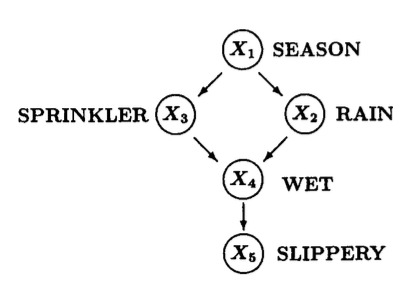
\includegraphics[width=\textwidth]{imgs/img8.png}
		\caption{A small causal Bayesian network}
		\label{fig:scbn1}
	\end{subfigure}
	\begin{subfigure}[t]{0.4\textwidth}
		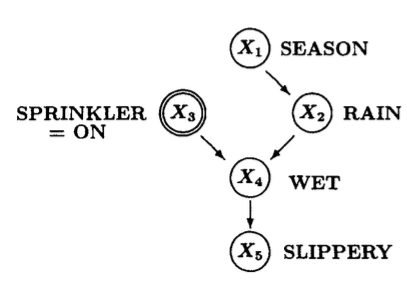
\includegraphics[width=\textwidth]{imgs/img9.png}
		\caption{After intervention Sprinkler := On}
		\label{fig:scbn2}
	\end{subfigure}
	\label{fig:scbn}
\end{figure}

All variables are binary (Yes/No) except for the season, which takes one of four values: summer/autumn/winter/spring. Thus, for this network:
\begin{align}
	P(x) = P(x_1)P(x_2|x_1)P(x_3|x_1)P(x_4|x_2,x_3)P(x_5|x_4)
\end{align}

Suppose we perform an intervention by forcibly turning on the sprinkler. Clearly, in this case we must remove the edge $x_1 \rightarrow x_3$, since now the season can no longer influence the sprinkler - essentially, through our \textbf{action} we have changed the physical law determining $x_3$. 

This highlights precisely the difference between observing $X_3=On$ and performing the action $do(X_3 = On)$: in the first case we simply condition in the original Bayesian network, while in the second - in the network modified by intervention. When we observe that the sprinkler is on, we might assume it's currently hot season, that it probably hasn't rained, etc. When we ourselves turn on the sprinkler, such assumptions naturally become groundless.

\define{Causal Bayesian Network} Let $P(v)$ be a probability distribution over variables $V$, and $P_x(v)$ be the distribution resulting from intervention $do(X=x)$. Denote by $P_*$ the set of all interventional distributions $P_* = \{P_x(v)| X \subset V, x = instance(X)\}$. A DAG G is called a causal Bayesian network compatible with $P_*$ if and only if $\forall P_x \in P_*$ the following holds:\\
1. $P_x(v)$ is Markov relative to G\\
2. $P_x(v_i) = 1 \ \forall V_i \in X$ if $v_i$ is consistent with $X=x$ \\
3. $P_x(v_i|pa_i) = P(v_i|pa_i) \ \forall V_i \notin X$, if $pa_i$ is consistent with $X=x$

These constraints on the set of interventions $P_*$ allow its compact representation as a single graph G, and straightforward computation of interventional distributions via the truncated factorization rule:
\begin{align}
	P_x(v) = \prod\limits_{\{i|V_i \notin X\}}P(v_i|pa_i) &, \ \forall v \text{ consistent with } x
\end{align} 

Let us show how this rule follows from the properties of causal Bayesian networks. Indeed, by property 1, $P_x(v) = \prod\limits_{i}P(v_i|pa_i)$. $P_x(pa_i) = \sum\limits_{v'_i}P_x(pa_i|v'_i)P(v_i)$. Note further that if $V_i \in X$, then $P(v'_i) = \delta(v'_i = v_i)$, and thus $P_x(pa_i) = P_x(pa_i|v_i)$ in this case, meaning $PA_i$ is independent of $V_i$ in the $P_x$ distribution. This in turn means that $P_x(v_i | pa_i) = P_x(v_i) = 1$, which is what we needed to show.

It is not difficult to prove the validity of the following two properties for G - a causal Bayesian network compatible with $P_*(v)$:

\textbf{Property 1}: $\forall i \ P(v_i|pa_i) = P_{pa_i}(v_i)$\\
Indeed, $P(v_i|pa_i) = P_{pa_i}(v_i|pa_i) = \frac{P_{pa_i}(v_i, pa_i)}{P_{pa_i}(pa_i)} = P_{pa_i}(v_i)$, where the first transition follows from condition 3 of the causal Bayesian network definition with $X = PA_i$, the second - because $P_{pa_i}(v_i) = \sum\limits_{PA_i}P_{pa_i}(v_i, PA_i) = P_{pa_i}(v_i, pa_i)$, since $P_{pa_i}$ takes nonzero values only when $PA_i = pa_i$, and accordingly $P_{pa_i}(pa_i) = 1$.

In essence, this property means that the observed distribution of variable $v_i$ given that we have observed $pa_i$ coincides with the distribution of $v_i$ when we externally set $PA_i = pa_i$.

\textbf{Property 2}: $\forall i, \ \forall S \subset V: S \cap (\{V_i\} \cup PA_i) = \emptyset \implies \ P_{pa_i, s}(v_i) = P_{pa_i}(v_i)$\\
By condition 3 we have $P_{pa_i,s}(v_i|pa_i) = P(v_i|pa_i)$.
Similarly to property 1, it is easy to show that $P_{pa_i,s}(v_i) = P_{pa_i,s}(v_i, pa_i)$. Further, $P_{pa_i,s}(v_i, pa_i) = P_{pa_i,s}(v_i|pa_i)P_{pa_i,s}(pa_i) = P_{pa_i,s}(v_i|pa_i)$, since by condition 2 $P_{pa_i,s}(pa_i) = 1$. Thus, $P_{pa_i,s}(v_i) = P_{pa_i,s}(v_i|pa_i) = P(v_i|pa_i) = P_{pa_i}(v_i)$ (the penultimate transition by condition 3, the last - similarly to property 1).

In essence, this property describes the concept of invariance: once we control $PA_i$ - all direct causes of $V_i$ - all other actions do not affect the behavior of $V_i$.

There is an important difference between causal and probabilistic relationships: causal relationships are more "stable". What does this mean? Essentially, causal relationships describe the mechanics of the external world, while probabilistic ones describe what we know/believe about the world. Thus, causal relationships do not change when we acquire new information - in this sense they are stable, at least as long as the physical laws (broadly speaking - the laws governing the environment) remain unchanged.

Here's an example from our simple causal Bayesian network: consider the causal relation $S_1$ "Turning on the sprinkler does not affect whether it rains", and the probabilistic relation $S_2$ "The sprinkler's state is independent of whether it rains". According to Figure \ref{fig:scbn1}, $S_2$ changes from False to True if we learn the current season, and back from True to False if we learn whether the pavement is wet. However, learning any of these facts does not affect the truth of $S_1$. 

\subsection*{Functional Causal Models}

A functional causal model consists of a set of equations of the form:

\begin{align}
	x_i = f_i(pa_i, u_i),& \  i=1..n
	\label{eq:causal_eq}
\end{align}

Here $pa_i$ is the set of variables directly determining the value of $X_i$, and $U_i$ represents noise associated with unobserved variables.

Let us compare the features of functional models with those of causal Bayesian networks. Consider three types of queries, from least to most demanding in terms of knowledge granularity:

1. Predictions - will the pavement be wet if the sprinkler is off?

2. Interventions - will the pavement be wet if we turn off the sprinkler?

3. Counterfactuals - would the pavement be wet if we had turned off the sprinkler, given that we know the pavement is slippery and the sprinkler is on?

\subsubsection*{Predictions}

From a functional causal model we construct a diagram by drawing edges from $PA_i$ to $X_i$; the resulting graph G is called a \textbf{causal diagram}. If G is a DAG, the corresponding model is called \textit{semi-Markovian}, and the values of $X$ are uniquely determined by the values of $U$, with $P(x)$ being uniquely determined through $P(u)$. If additionally the $U$ variables are mutually independent, the model is called \textit{Markovian}.

\begin{theorem}
	\textbf{Causal Markov Condition}\\
	Any Markovian causal model M generates a distribution $P(x_1...x_n)$ that satisfies the parental Markov condition relative to the diagram G constructed from M. That is, $X_i \independent Y | PA_i$ for any $Y$ not containing descendants of $X_i$.
	\label{th:causal_markov_condition}
\end{theorem}

Indeed, $PA_i,U_i$ uniquely determine the value of $X_i$, so certainly $P(x_1...x_n, u_1..u_n)$ is Markov compatible with the extended graph $G(X,U)$ (recall that this simply means the distribution factorizes according to the graph). The theorem's statement is then easily proved using the d-separation criterion in the extended graph and the theorem about probabilistic consequences of d-separation.
$\blacksquare$

The Markov property of causal models can be guaranteed if we agree on two modeling rules:

1. If $x_i$ and $x_j$ are dependent, then either one is the cause of the other (not necessarily directly), or there exists a third variable that is their common cause (no correlation without causation and no mutual causation).

2. If more than one variable is a consequence of a given variable $y$, then this variable must be included in the model, i.e., $y \notin U$ - otherwise we would observe correlations between $x_i, x_j$ that the model cannot explain, for which $y$ is the common cause.

The second assumption guarantees that $U_i \independent U_j$. The first ensures there are no cyclic dependencies, thus yielding a Markovian causal model.

What are the advantages of using functional models compared to causal Bayesian networks?  

First, functional specifications are typically more concise and contain fewer parameters.

Second, reasoning about conditional independence is simpler in functional models because it's more natural for humans to derive such assumptions from the absence of unobserved common causes. It's much easier for a person to verify that all direct causes of an event have been accounted for than to check that a variable is independent of its non-descendants given its immediate parents.

Finally, when environmental laws change, it's easier to incorporate these changes in a functional description than in a purely probabilistic one, since in the former case typically only a few equations need to be updated.

Nevertheless, prediction remains the simplest of the three tasks and can be addressed in terms of conditional probabilities, without necessarily requiring structural equations or even causal Bayesian networks (ordinary ones will suffice).

\subsubsection*{Interventions}

Interventions are easily described in the language of functional models. For all variables whose behavior is determined by actions, we simply remove the corresponding equations and replace them with $x_i = c_i$. 

Beyond this convenience, functional models offer other advantages. First, greater flexibility: by moving beyond Markovian models, we can describe cyclic dependencies as well, thereby addressing policy-related questions.

Second, interventions that change equation parameters are more intuitive than those that change conditional probabilities, since equations are typically viewed as describing relatively stable physical processes, unlike conditional probabilities. We usually regard conditional probabilities as derived from the joint distribution rather than as generating it. 

Ordinary Bayesian networks are insufficient for studying the effects of interventions - we need causal Bayesian networks or structural equations.

\subsubsection*{Counterfactuals}

Counterfactual statements fundamentally cannot be defined in terms of stochastic causal models (stochastic meaning the same as Bayesian networks). Consider a simple example: a model with two variables $X$ - whether a person received treatment or not, and $Y$ - whether they ultimately survived. Suppose an individual Joe died after receiving medication, and we want to answer the counterfactual question "What would be the probability that Joe \textbf{would have} survived if he had not been given the medication?"

Clearly, answering this question from the available data is impossible: Joe died, and we have no information about what would have happened had he not received the medication. Rephrasing the question in terms of the frequency of similar counterfactual events in the population doesn't help in this case, which is why many statistical analysts have long viewed counterfactual questions as metaphysical - impossible to answer through direct testing.

Nevertheless, in everyday life we constantly use counterfactual statements, suggesting that such statements are meaningful and capable of conveying useful information or being derived from some information about the world.

In our example, let $P(y|x) = 0.5 \ \forall x, y$. Then clearly $P(x,y) = 0.25$. Consider two functional models, each generating this joint distribution but leading to different values of the desired counterfactual probability Q - that a subject who died after treatment ($x=1, y=1$) would not have died ($y = 0$) if they had not been treated ($x=0$). 

The Bayesian network describing this distribution is shown in \ref{fig:treatment_sample_bn}

\begin{figure}[!tbph]
	\centering
	\begin{subfigure}[t]{0.3\textwidth}
		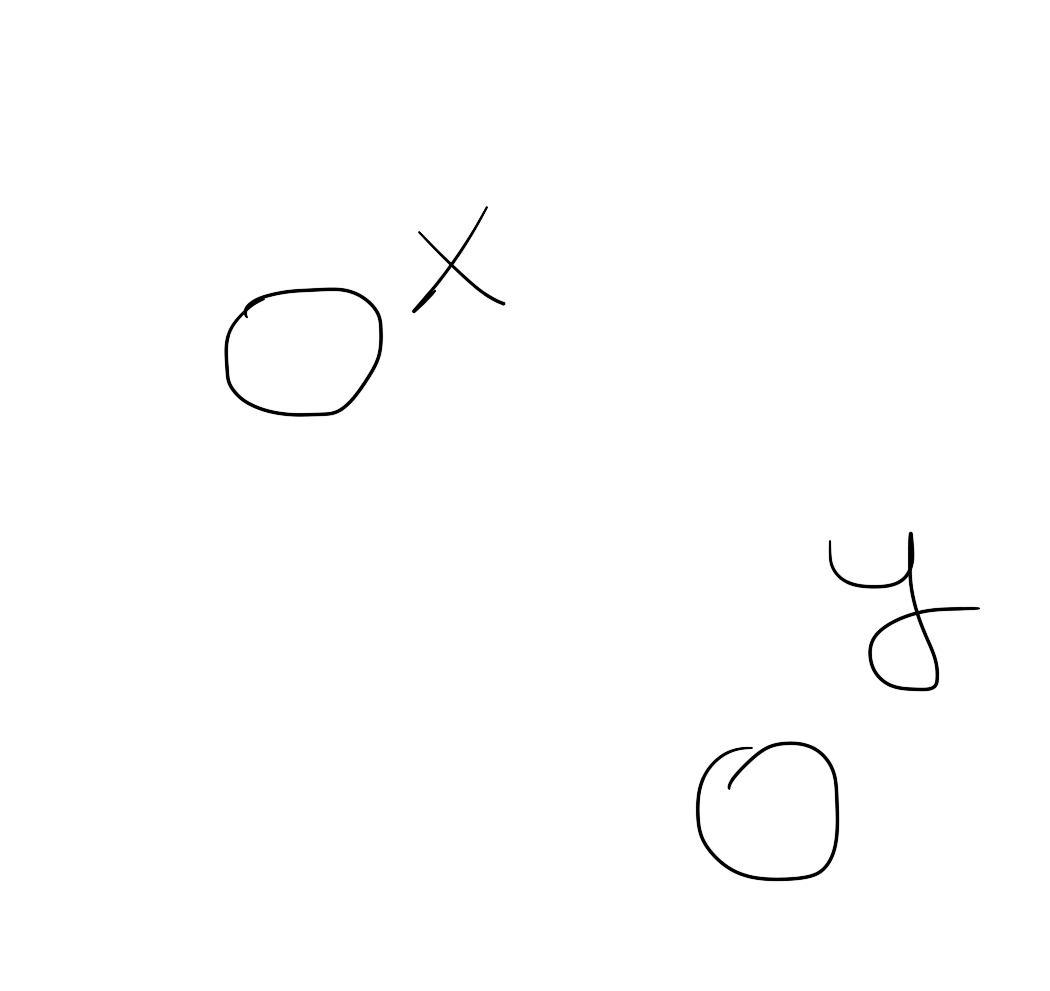
\includegraphics[width=\textwidth]{imgs/img12.png}
		\caption{Bayesian network for the described distribution}
		\label{fig:treatment_sample_bn}
	\end{subfigure}
	\begin{subfigure}[t]{0.25\textwidth}
		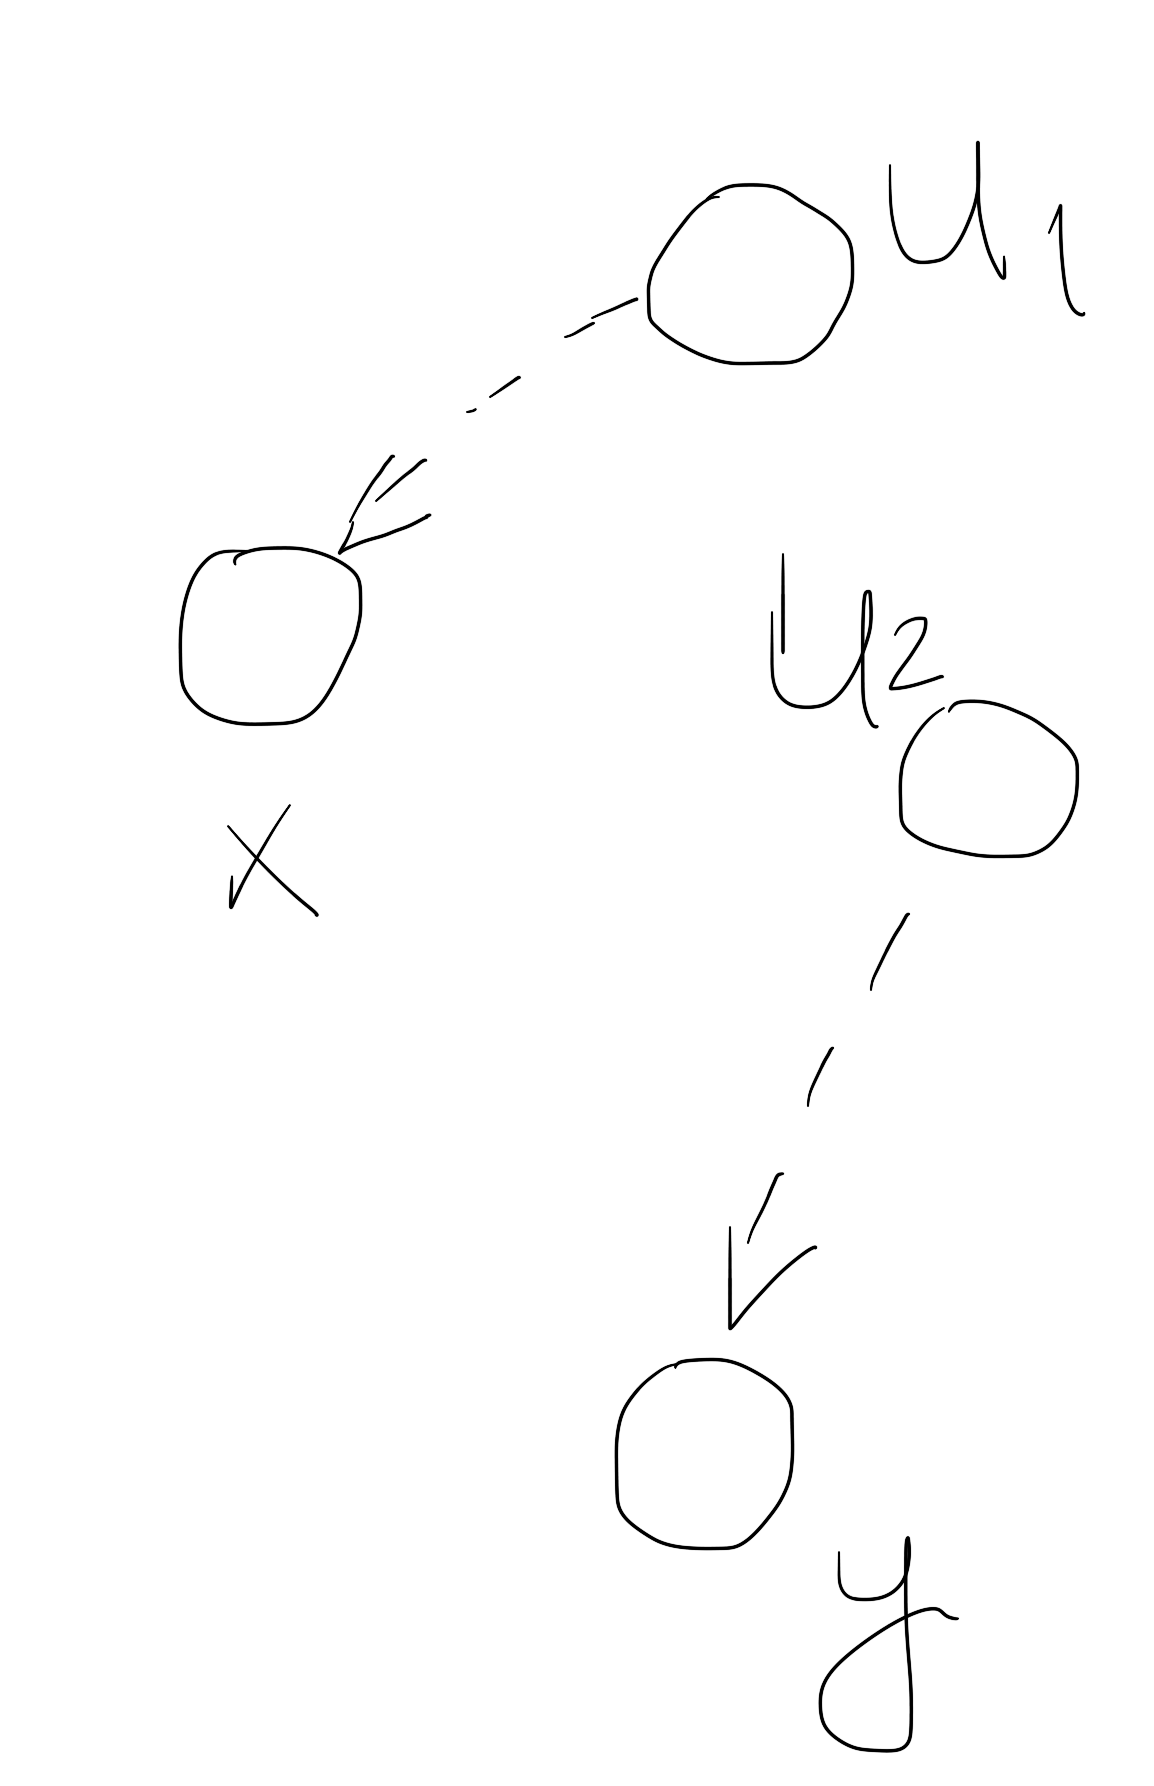
\includegraphics[width=\textwidth]{imgs/img13.png}
		\caption{Causal diagram for Model 1}
		\label{fig:treatment_sample_cm1}
	\end{subfigure}
	\begin{subfigure}[t]{0.25\textwidth}
		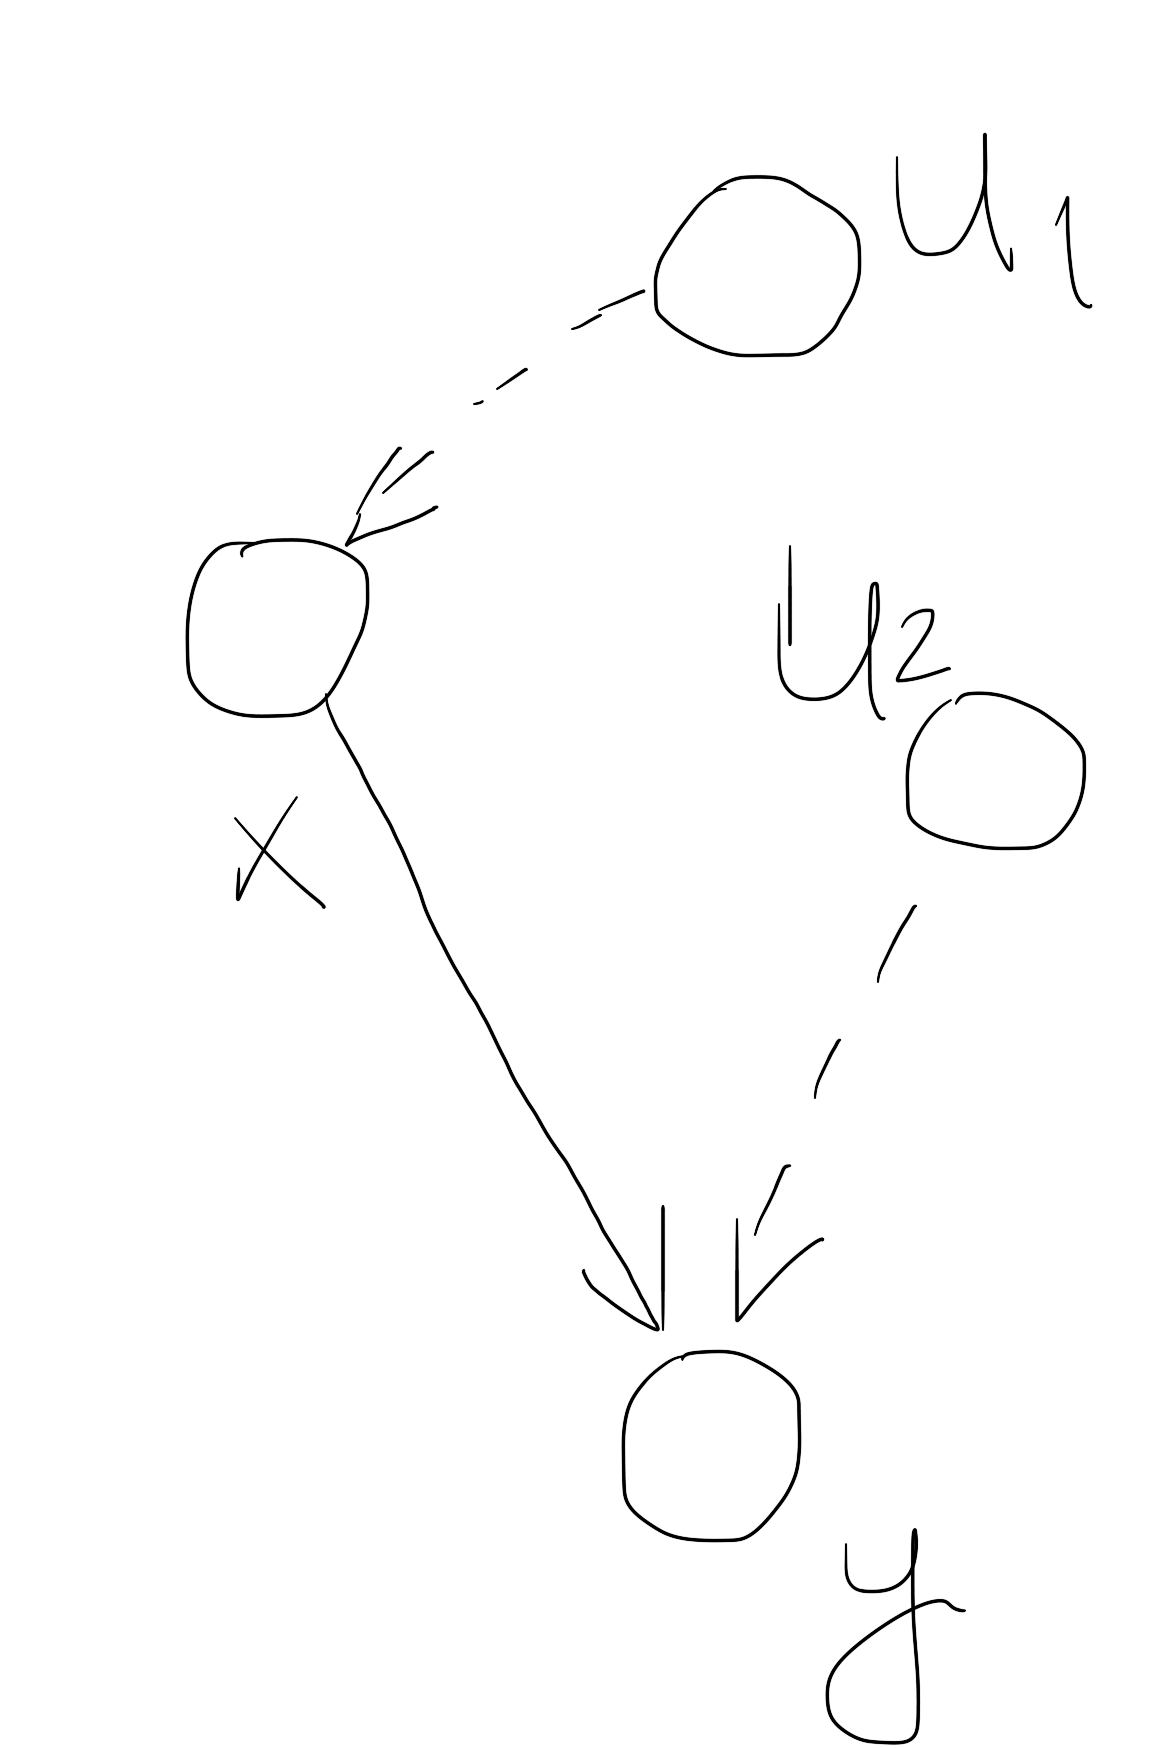
\includegraphics[width=\textwidth]{imgs/img14.png}
		\caption{Causal diagram for Model 2}
		\label{fig:treatment_sample_cm2}
	\end{subfigure}
\end{figure}


\textbf{Model 1}
\begin{align}
	\begin{split}
		x = u_1\\
		y = u_2
	\end{split}
\end{align}

\textbf{Model 2}
\begin{align}
	\begin{split}
		x &= u_1\\
		y &= u_2x + (1- x)(1- u_2)
	\end{split}
\end{align}

In the first model, the outcome does not depend on the treatment; in the second model, the outcome for any patient depends on the treatment. The point is that Model 2 describes a mixture of two subpopulations: one ($u_2 = 0$) where the patient recovers only if they take the medication, and another ($u_2 = 1$) where the patient recovers only if they are not given the medication.

The treatment effect differs between these two models. In Model 1, $y = u_2$ and the treatment does not affect the outcome, so replacing $X$ from 1 to 0 for those who died and were treated will not change $y = 1 = u_2$ from 1 to 0, hence $Q = 0$. In Model 2, however, replacing $X$ from 1 to 0 for those who died (which is the $u_2 = 1$ subpopulation) changes the tragic outcome to a positive one ($y = 1 \cdot x = 0$), meaning the effect of no treatment would be $Q = 1$.

As we can see, the stochastic model does not allow computing counterfactual probabilities in this case: knowledge of the process behind $P(y|x)$ is needed. On the other hand, causal structural models allow computing such quantities. We performed this computation in three steps: first, we applied the available data $e: \{x=1, y=1\}$. Knowing this, we derived the compatible values of $U_1, U_2$—in this case, only $u_1 = 1, u_2 = 1$. Second, we substituted $x=1$ into the structural equations, ignoring the equation for $X$: $x = u_1$. Finally, we solved the equations for $y$ and obtained $y \equiv 0$, meaning the probability of recovery in this scenario is certain.

This approach generalizes to defining the probability of any counterfactual $Y = y$ given data $e$ under condition $X=x$ in a structural model in three steps.

1. \textbf{Abduction} - replace $P(u) \leadsto P(u|e)$

2. \textbf{Action} - replace the equations defining $X$ with $X=x$

3. \textbf{Prediction} - use the modified model to compute the probability $Y = y$.

Using temporal metaphors, the first step is explaining the past given the available evidence/data; the second step is minimally altering the course of history to align the world with $X = x$; the third step is predicting the future $Y$ given our new understanding of the past and our alternative present.

Overall, this is the most complex of the three tasks and cannot be solved without invoking the mechanism of structural equations.

\subsection*{Causal and Statistical Terminology}

\define{Probabilistic parameter} - any quantity defined through the joint distribution of variables.

\define{Statistical parameter} - any quantity defined through the joint distribution of observed variables, without any assumptions about the existence/non-existence of unobserved variables. Examples include conditional expectation $E(Y|x)$, regression coefficient $r_{XY}$, the value of the probability density at $x = 0, y = 1$.

\define{Causal parameter} - any quantity defined through a causal model (given as structural equations) as in \ref{eq:causal_eq} and not simultaneously a statistical parameter. Examples include parameters of the function $f_i(pa_i, u_i)$, whether $X_9$ influences $X_3$ for some $u$, the expected value of $Y$ under intervention $do(X=0)$.

\define{Statistical assumption} - an assumption about the joint distribution of observed variables: for example, that it is Markov relative to some DAG, or is multivariate normal.

\define{Causal assumption} - any constraint on the causal model that cannot be represented by statistical assumptions. For example, that $f_i$ is linear or that $x_3 \notin pa_4$. Causal assumptions may or may not have statistical consequences. In the former case, the causal assumption is said to be "testable" or "falsifiable." Often, though not always, causal assumptions are falsifiable through experiment; in this case, we speak of "experimental falsifiability." For example, the assumption that $X$ has no effect on $E[Y]$ in the previously discussed Model 2 is falsifiable by experiment, whereas the assumption "$X$ can cure a certain subject in the population" is not.

\subsection*{Two Mental Barriers to Causal Analysis}

There are two difficulties we face: first, behind every causal statement lie causal assumptions that are not derived from the joint distribution and, accordingly, cannot be verified using observed data alone. These assumptions are provided by humans, meaning we must rely on some expert opinion.

Second, a new notation is needed for the mathematical description of causal theory: as we have found, the purely probabilistic language is insufficient. For example, in the language of probability theory (i.e., through distribution functions), it is impossible to express the causal connection between a symptom and a disease: we can only describe their dependence through $P(disease | symptom)$, but we cannot distinguish whether this dependence is causal or statistical.

\section{Theory of Causal Inference}

\subsection*{Intuition}
Let's start with the intuition behind cause-and-effect relationships. Usually, a necessary condition is temporal dependence—the cause precedes the effect. However, this is clearly not always a sufficient condition for a causal relationship, so the question remains: how to establish it?

Is it even possible to identify cause-and-effect relationships? In fact, yes. Consider an example where there are three events $A, B, C$, and we know that $A$ is dependent with $B$, $B$ is dependent with $C$, but $A$ and $C$ are independent. In this case, with a bit of thought, it turns out that the simplest graph describing such a configuration looks like \ref{fig:abc}.

\begin{figure}[h]
	\begin{center}
		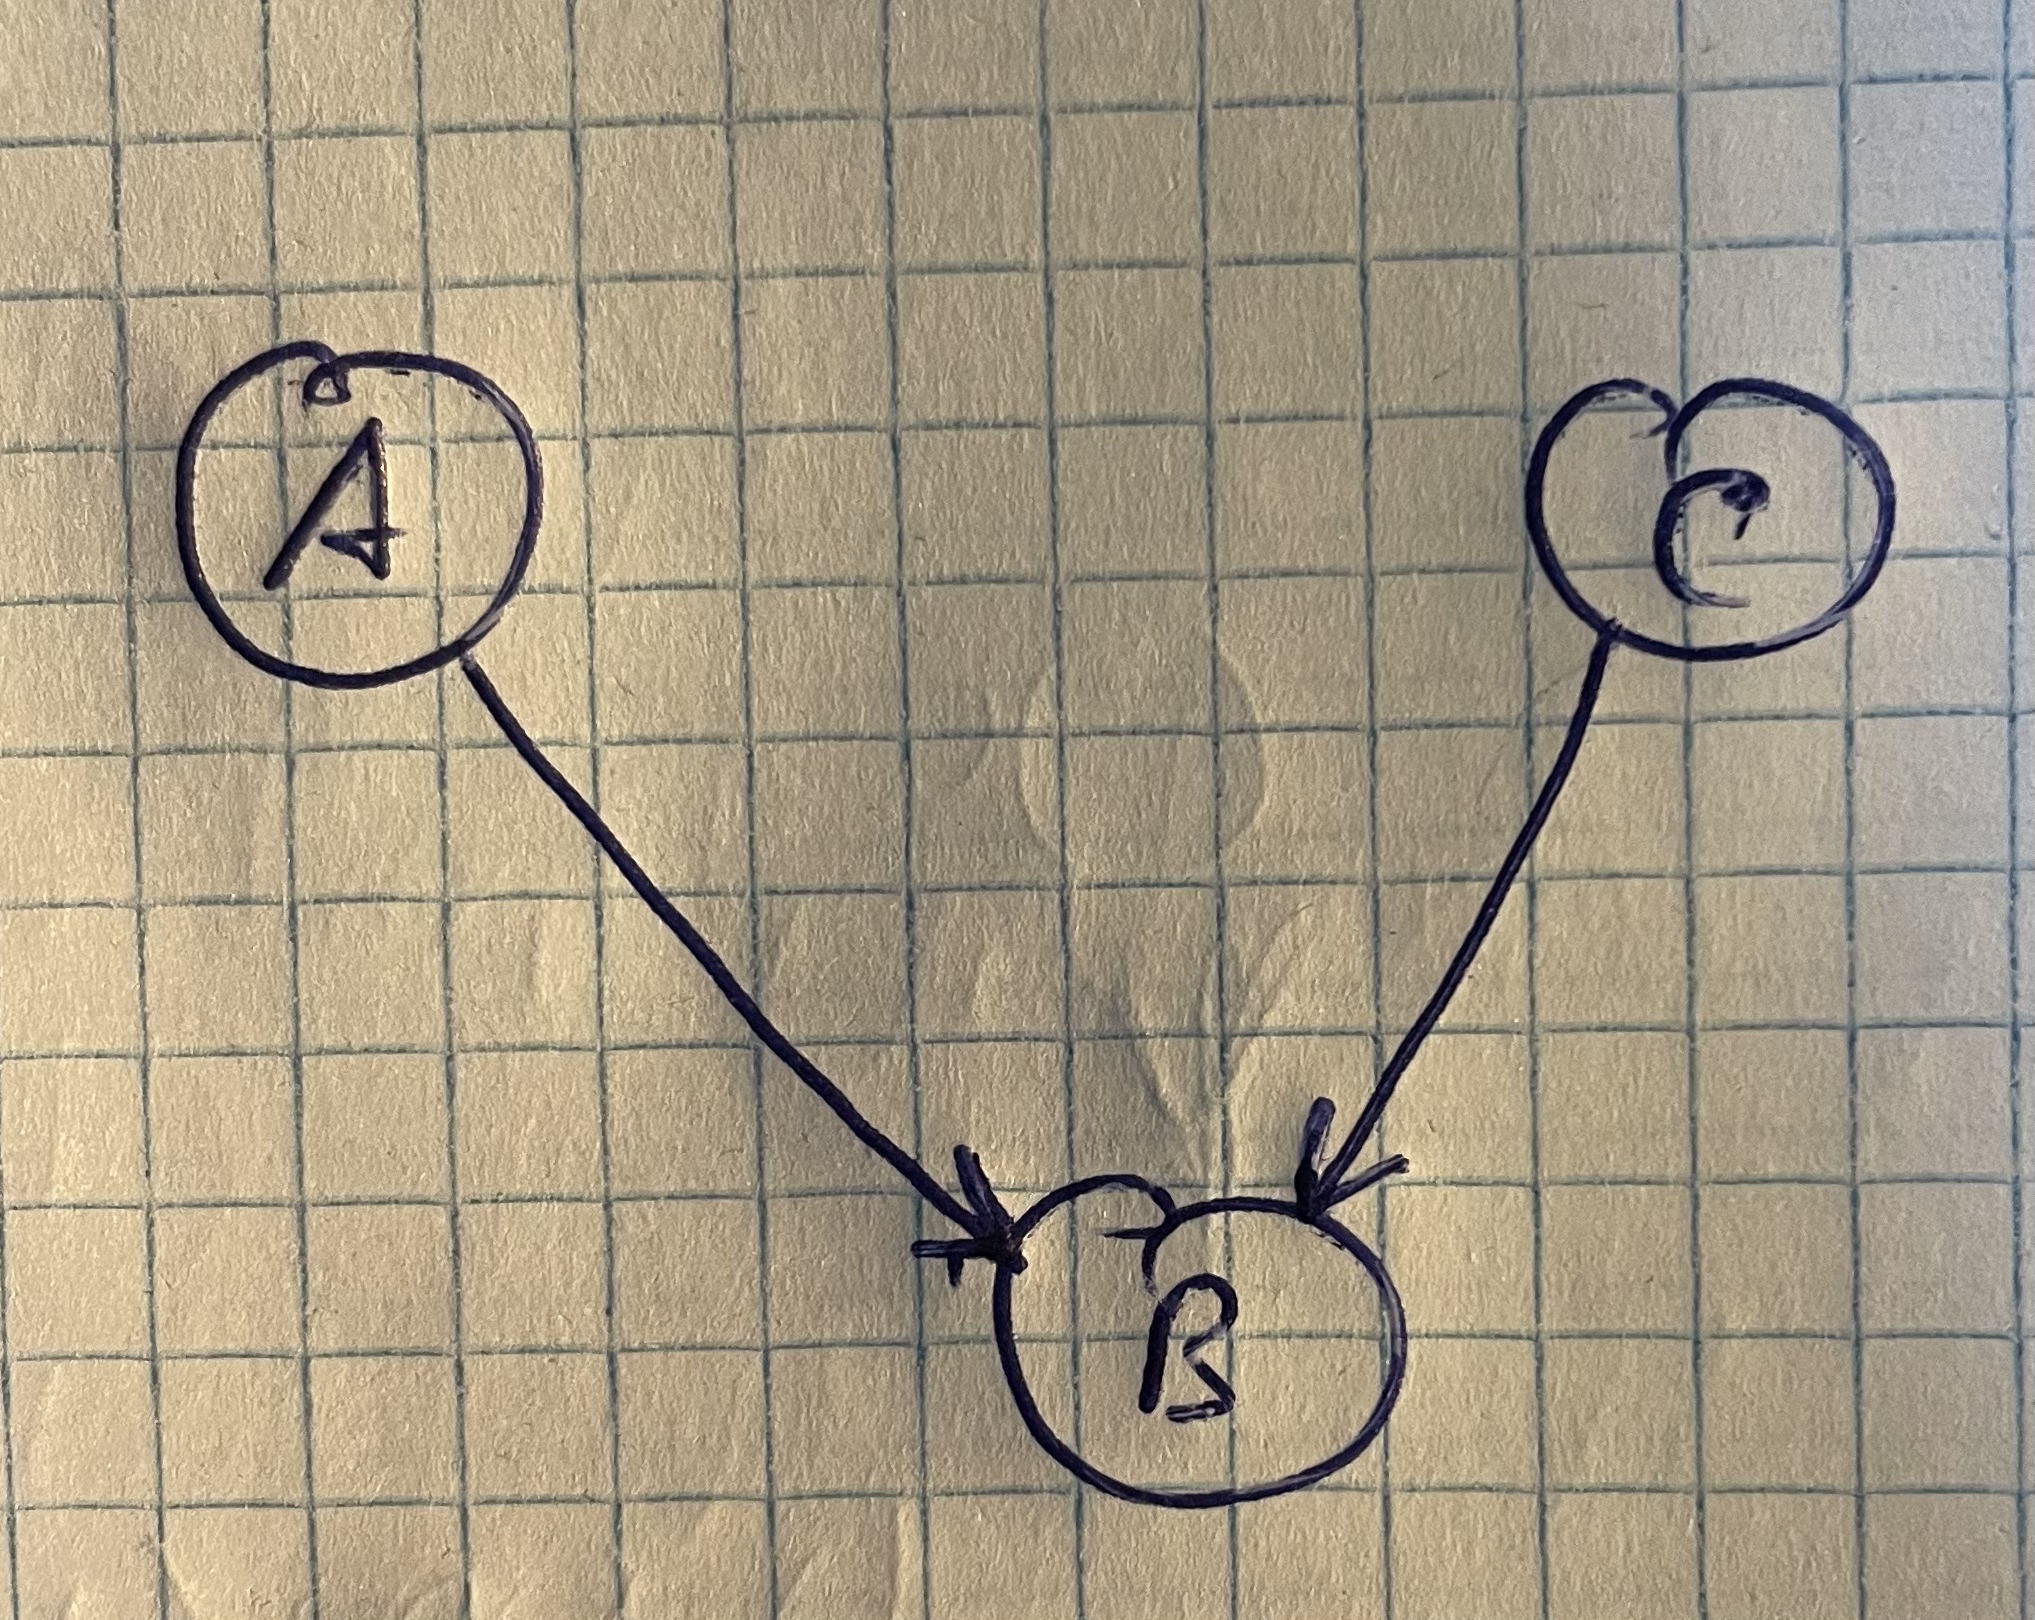
\includegraphics[scale=0.1]{imgs/img1.png}
	\end{center}
	\caption{A, C are unconditionally independent but dependent given observed effect B}
	\label{fig:abc}
\end{figure}

\subsection*{Framework}

We will consider the task of determining cause-and-effect relationships as an induction game (inductive in the sense that some general rule is inferred from examples), which a scientist plays with nature (a beautiful formulation, of course XD). It is assumed that nature has stable cause-and-effect mechanisms that can be defined by functional dependencies between variables, some of which are unobservable.

\define{Causal structure} of a set of variables $V$ is a DAG where vertices correspond to variables, and edges correspond to direct functional dependencies between the corresponding variables.

A causal structure is roughly a blueprint for a \textbf{causal model}—a precise definition of how some variables influence others.

\define{Causal model} is a pair $(D, \Theta_D)$ consisting of a causal structure $D$ and a set of parameters $\Theta_D$ corresponding to it, i.e., describing specific functional dependencies between variables $V$ as $x_i = f_i(pa_i, u_i)$ $\forall x_i \in V$, where $PA_i$ are the parents of $x_i$ according to $D$, $U_i$ is random noise, the probability distribution over which is also determined by $\Theta_D$, $U_i \independent U_j$.

The noise affecting the values of variables can be viewed, for example, as a consequence of the unobservability of some variables. Such a model, according to the earlier definition, is Markovian, and therefore, by Theorem \ref{th:causal_markov_condition}, defines a distribution that is Markov consistent with $D$.

Now, the task facing the hypothetical scientist can be formulated as recovering the causal structure and then the model, given that they observe only the values of some subset of variables $O \subset V$.

\subsection*{Model Selection (Occam's Razor)}

Generally speaking, since $V$ is unknown, one can come up with infinitely many different models that could fit the given (empirically determined) distribution $P(O)$ by variously introducing hidden variables. For example, one could introduce a single hidden variable $U$ that would be the cause of all observed variables $O$, with no cause-and-effect relationships between the observed variables in such a model; the causal structure for such a model is shown in \ref{fig:useless_model}.

\begin{figure}[h]
	\begin{center}
		\includegraphics[scale=0.1]{imgs/img2.png}
	\end{center}
	\caption{A rather useless causal structure}
	\label{fig:useless_model}
\end{figure}

On the other hand, assuming $V=O$ but having no temporal hints, the scientist cannot dismiss the possibility that the underlying structure is a complete DAG where all vertices are connected to all others in arbitrary order—such a structure can mimic the behavior of any structure.

The idea of model selection is that, in some sense, it should be the simplest/minimal relative to the observed data.

Next, we introduce a not entirely formal definition of inferred causality (for now assuming all variables are observable).

\define{Inferred causality (preliminary)} Variable $X$ has a causal influence on variable $Y$ if there exists a directed path from $X$ to $Y$ in any minimal \textbf{causal} structure consistent with the data.

\define{Latent structure} is a pair $L = (D, O)$, where $D$ is a causal structure over $V$, $O \subset V$ is the set of observed variables.

\define{Structure preference} Structure $L = (D, O)$ is preferred over structure $L' = (D', O')$ (denoted $L \preceq L'$) if $D'$ is equivalent to $D$ on the set of observed variables $O$, i.e., if and only if $\forall \Theta_D \ \exists \Theta_{D'} : P_{[O]}((D', \Theta_{D'})) = P_{[O]}((D, \Theta_{D}))$.

Latent structures are called equivalent if $L \preceq L'$ and $L' \preceq L$.

\define{Minimality} of structure $L$ relative to a class of structures $C$ means its preference over all other structures in this class: $\forall L' \in C \ L \preceq L'$.

\define{Consistency} of latent structure $L = (D, O)$ with distribution $\hat P$ over $O$ means the possibility of embedding $\hat P$ in this latent structure, i.e., that $\exists \Theta_D : P((O, \Theta_D)) = \hat P$.

\define{Inferred causality} Given $\hat P$ over $O$, variable $X$ has a causal influence on variable $Y$ if there exists a directed path from $X$ to $Y$ in any minimal \textbf{latent} structure.

It should be noted that the expressive power of a latent structure is higher the fewer independencies between variables are encoded in it: thus, structures with fewer independencies, consistent with the data, will be less preferred than structures with more independencies in the causal structure.

\subsection*{Stable Distributions}

The concept of minimality of latent structures allows for correct and consistent inferences about causal relationships between variables. However, this is not always computationally simple—there can be very many different structure configurations, and checking each for minimality can be very expensive. Moreover, it might turn out that the true process that generated the data was indeed produced by a model different from the minimal one? To simplify our lives, we introduce another principle besides minimality—the principle of \textit{stability}.

Let's start with a small example. Consider a process where there are two fair coins. The set of events will be the outcome of coin $A$, the outcome of coin $B$, and event $C$—"the coins landed on the same side." It's easy to see that any pair of variables is unconditionally independent but dependent given the third variable (for example, $P(A=1) = P(A=1|B) = 0.5\ \forall B$, but $P(A=1|B=1) =0.5\neq P(A=1|C=1,B=1) = 1$). Thus, any of the structures in \ref{fig:choice} is admissible from the data perspective and is minimal. At the same time, if we slightly tweak the distribution parameters, for example, making $P(A=1) = 0.6, P(A=0)=0.4$, then the structure where $C$ and $B$ are unconditionally independent will no longer fit, as we will have $P(C=1) = 0.5$, but $P(C=1|B=1) = 0.6$. Similarly, we can tweak the probabilities for the second coin, making it not entirely fair, and discard the model where $A$ and $C$ are independent.

\begin{figure}[h]
	\begin{center}
		\includegraphics[scale=0.07]{imgs/img3.png}
	\end{center}
	\caption{Which of the three causal structures to choose?}
	\label{fig:choice}
\end{figure}

To resolve such ambiguities, the concept of stability is introduced:

\define{Stability (of a distribution)} Let $I(P)$ be the set of all independence relations of variables defined by $P$. A causal model $M = (D, \Theta_D)$ generates a stable distribution if and only if in $P((D, \Theta_D))$ there are no extra independencies, i.e., $I(P((D, \Theta_D))) \subset I(P(D, \Theta_{D'}))\ \forall \Theta_{D'}$.

In essence, when varying parameters from $\Theta$ to $\Theta'$, no independencies should break if the distribution is stable. What's unclear is how to choose which probabilities to tweak: presumably those that are not zero? Then indeed, from stability, only one of the three options in the above example remains.

Stability means that the distribution $P$ has an \textbf{ideal} representation as a DAG, i.e., the graph is not just an I-map but also a D-map, and thus is isomorphic to the distribution.

\subsection*{Reconstruction of Causal Structure (DAG)}

When all variables are observable, if we use the principles of minimality and stability, we will always obtain a unique (up to equivalence) causal structure (equivalent structures are those that share the same independencies, i.e., the same skeleton and v-structures).

Since the underlying structure may have equivalents, the obtained DAG will not be uniquely determined, so the best we can do is define its equivalence class. Such an equivalence class is called a \textbf{pattern}, and it is a partially directed graph (only those edges that are directed the same way in all graphs of this equivalence class are oriented).

\textbf{IC (Inductive Causation) Algorithm}

\textbf{Input:} $\hat P$—a stable distribution over variables $V$.

\textbf{Output:} $H(\hat P)$—a pattern consistent with $\hat P$.

\textbf{Step 1:} Construct an undirected graph $D$ on vertices $V$. Connect any two vertices $a, b$ with an edge if $\not \exists S_{ab} \subset V \backslash \{a,b\}:\ a \independent b | S_{ab}$.

\textbf{Step 2:} For any two vertices $a, b \in V: (a,c) \not \in E$, check their common neighbors $c: (a,c)\in E, (b,c) \in E$ and verify whether $c \in S_{ab}$ or not: if not, orient edges $a,c$ and $b,c$ towards $c$ (i.e., create a new $v$-structure).

\textbf{Step 3:} Orient the remaining edges if this can be done unambiguously under the conditions:
\begin{itemize}
	\item Acyclicity
	\item Not adding new $v$-structures
\end{itemize}

The first step is to build the skeleton of the graph—indeed, we should only connect vertices that are not separable by any set of other vertices. The second step is to orient all mandatory v-structures—because if $c \notin S_{ab}$, then $a - c - b$ must be blocked without conditioning on $c$, meaning $a \rightarrow c \leftarrow b$. The third step simply iteratively adds orientations to edges that can be unambiguously determined after all previous manipulations. Here, we do not add new v-structures, as all necessary ones were added in Step 2.

\subsection*{Reconstruction of Latent Structure}

When nature decides to "hide" some subset of variables, the observed distribution $\hat P$ may no longer be stable relative to the observed set of variables $O \subset V$.

\define{Projection of latent structure} $L_{[O]} = (D_{[O]}, O)$ for structure L is a latent structure with the following properties:

1. Any unobserved variable in $D_{[O]}$ is a common cause of \textit{exactly two} observed variables.

2. For any stable distribution $P$ generated by $L$, there exists a distribution $P'$ generated by $L_{[O]}$ that has the same independencies as $P$: $I(P_{[O]}) = I(P'_{[O]})$.

\begin{theorem}
	Any latent structure has at least one projection.
\end{theorem}

We will leave this statement without proof for now.
$\blacksquare$

Projections are conveniently represented as a bidirected graph where vertices correspond only to observed variables. Any bidirected edge in the graph indicates the existence of a common hidden cause for two observed variables.

It can be shown that having a projection of an arbitrary minimal latent structure generating $\hat P$, we can label the edges of the projection such that this labeling can be used to check for the presence of a causal path in any minimal model for $\hat P$. To construct a projection with subsequent edge labeling, there is the $IC^*$ algorithm, which divides edges into four types:

1. Labeled arrow $a \xrightarrow{*} b$—indicates the presence of a directed edge from $a$ to $b$ in the underlying model.

2. Unlabeled arrow $a \rightarrow b$—indicates either the presence of a directed edge in the underlying model or the existence of a common hidden cause $a \leftarrow L \rightarrow b$.

3. Unlabeled bidirected arrow $a \leftrightarrow b$ indicates the presence of a common hidden cause in the underlying model $a \leftarrow L \rightarrow b$.

4. Unoriented edge $a - b$ means that in the underlying model there is either an edge $a \rightarrow b$, or $a \leftarrow b$, or a common cause $a \leftarrow L \rightarrow b$.

\textbf{IC$^*$ (Inductive Causation with Latent Variables) Algorithm}

\textbf{Input:} $\hat P$—a distribution over variables $O$, stable relative to some latent structure.

\textbf{Output:} $core(\hat P)$—a labeled pattern consistent with $\hat P$.

\textbf{Step 1:} Construct an undirected graph $D$ on vertices $O$. Connect any two vertices $a, b$ with an edge if $\not \exists S_{ab} \subset V \backslash \{a,b\}:\ a \independent b | S_{ab}$.

\textbf{Step 2:} For any two vertices $a, b$ not connected by an edge but sharing a common neighbor $c$, check whether $c \in S_{ab}$. If not, then direct arrows towards $c$, forming a v-structure: $a \rightarrow c \leftarrow b$; otherwise, do nothing.

\textbf{Step 3:} In the obtained partially oriented graph, orient all possible edge ends iteratively by adding arrows according to two rules:

1. For any pair $a, b$ of vertices not connected by an edge, if $a \rightarrow c$ and there is no arrow from $b \rightarrow c$, then add arrow $c \xrightarrow{*} b$.

2. If $a,b$ are adjacent and there exists a directed path $a \xrightarrow{*} ... \xrightarrow{*} b$ consisting only of labeled arrows, then add $a \rightarrow b$.

\subsection*{Local Criterion for Causal Inference}

\define{Potential cause} Variable $X$ is a potential cause of $Y$ if the following conditions hold:

1. $\not \exists S: X \independent Y | S$, i.e., $X,Y$ are dependent in any context. Here, context means a set of variables with specific values.

2. There exists a context $S$ and a variable $Z$ such that:

- $X \independent Z | S$

- $Y \not \independent Z | S$

For better understanding, refer to Figure \ref{fig:x_potential_cause_of_y}: clearly, $Y$ \textit{cannot} be the cause of $X$, as otherwise there would exist an unblocked $S$ path $Z \leadsto Y \rightarrow X$, meaning either $X$ is the true cause of $Y$, or they are accidentally associated due to a common unobserved cause.

\begin{figure}[h]
	\begin{center}
		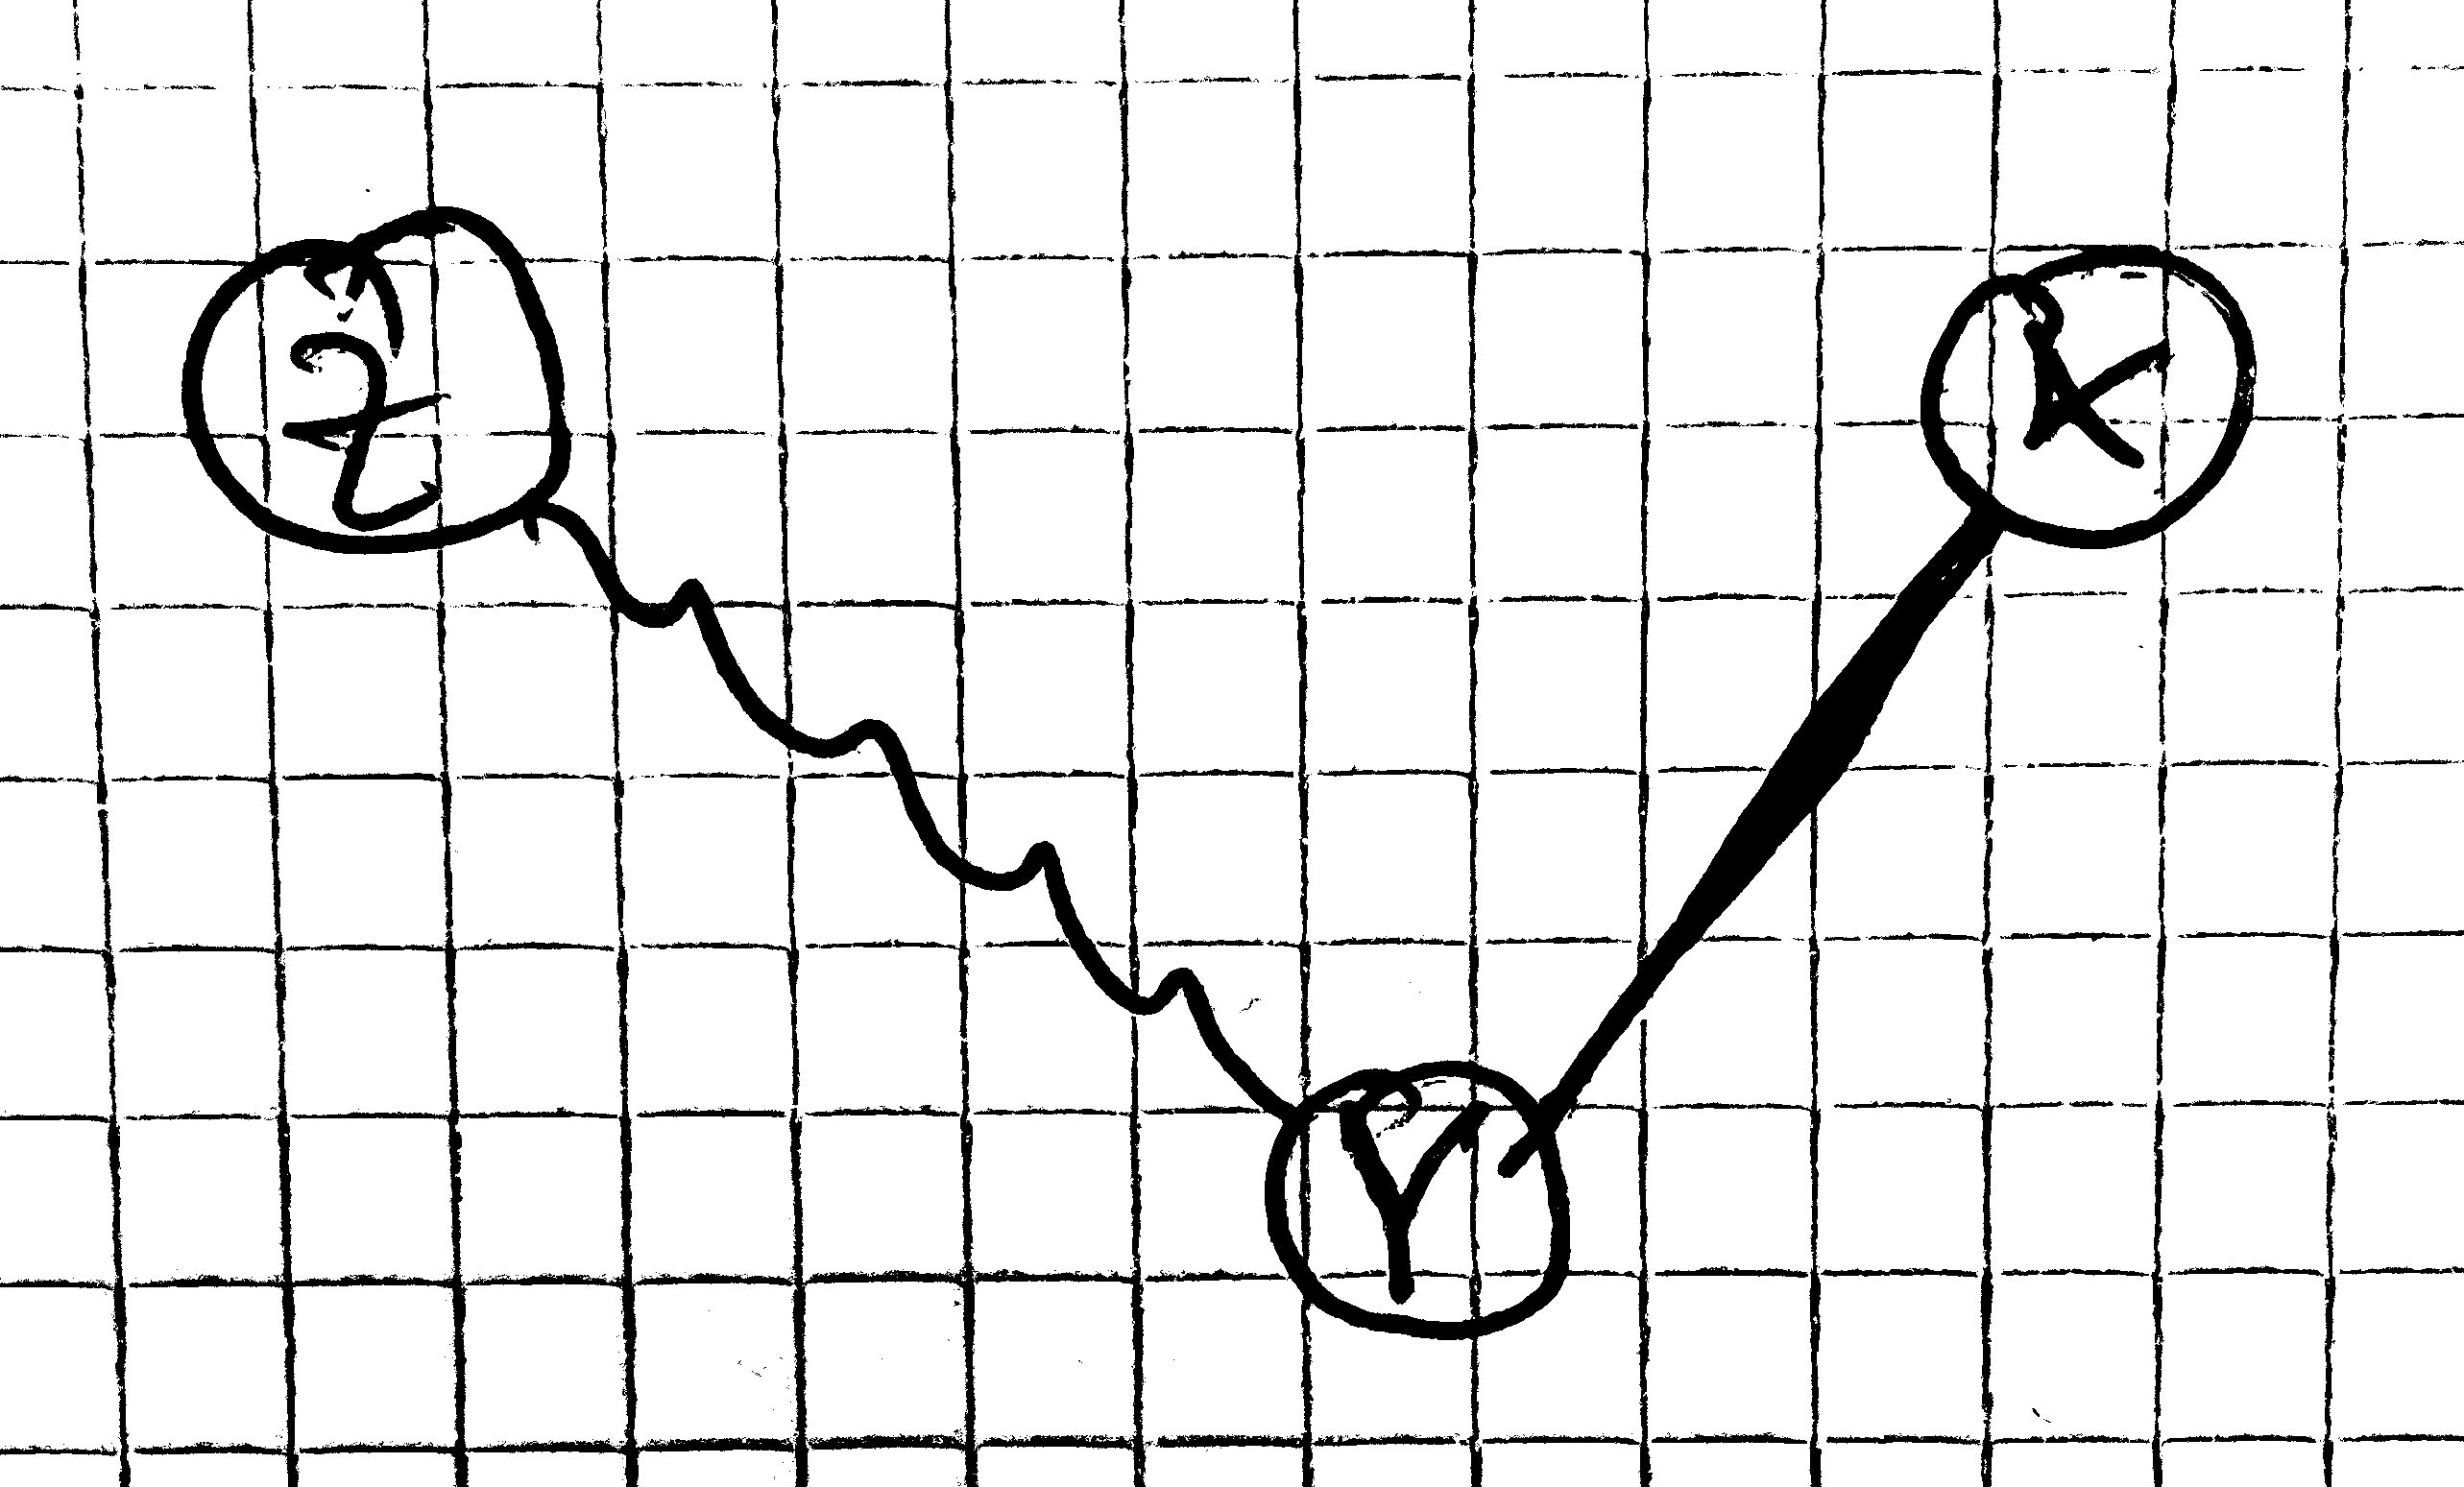
\includegraphics[scale=0.07]{imgs/img17.png}
	\end{center}
	\caption{X is a potential cause of Y, Y definitely cannot be the cause of X}
	\label{fig:x_potential_cause_of_y}
\end{figure}

\define{Genuine cause} Variable $X$ has a genuine causal influence on variable $Y$ if there exists a variable $Z$ such that one of the following two conditions holds:

1. $X, Y$ are dependent in any context, and there exists a context $S$:

* $Z$ is a potential cause of $X$ as per the previous definition.

* $Z \not \independent Y | S$

* $Z \independent Y | S \cup X$

2. $X, Y$ are in the transitive closure of the first condition.

\begin{figure}[h]
	\begin{center}
		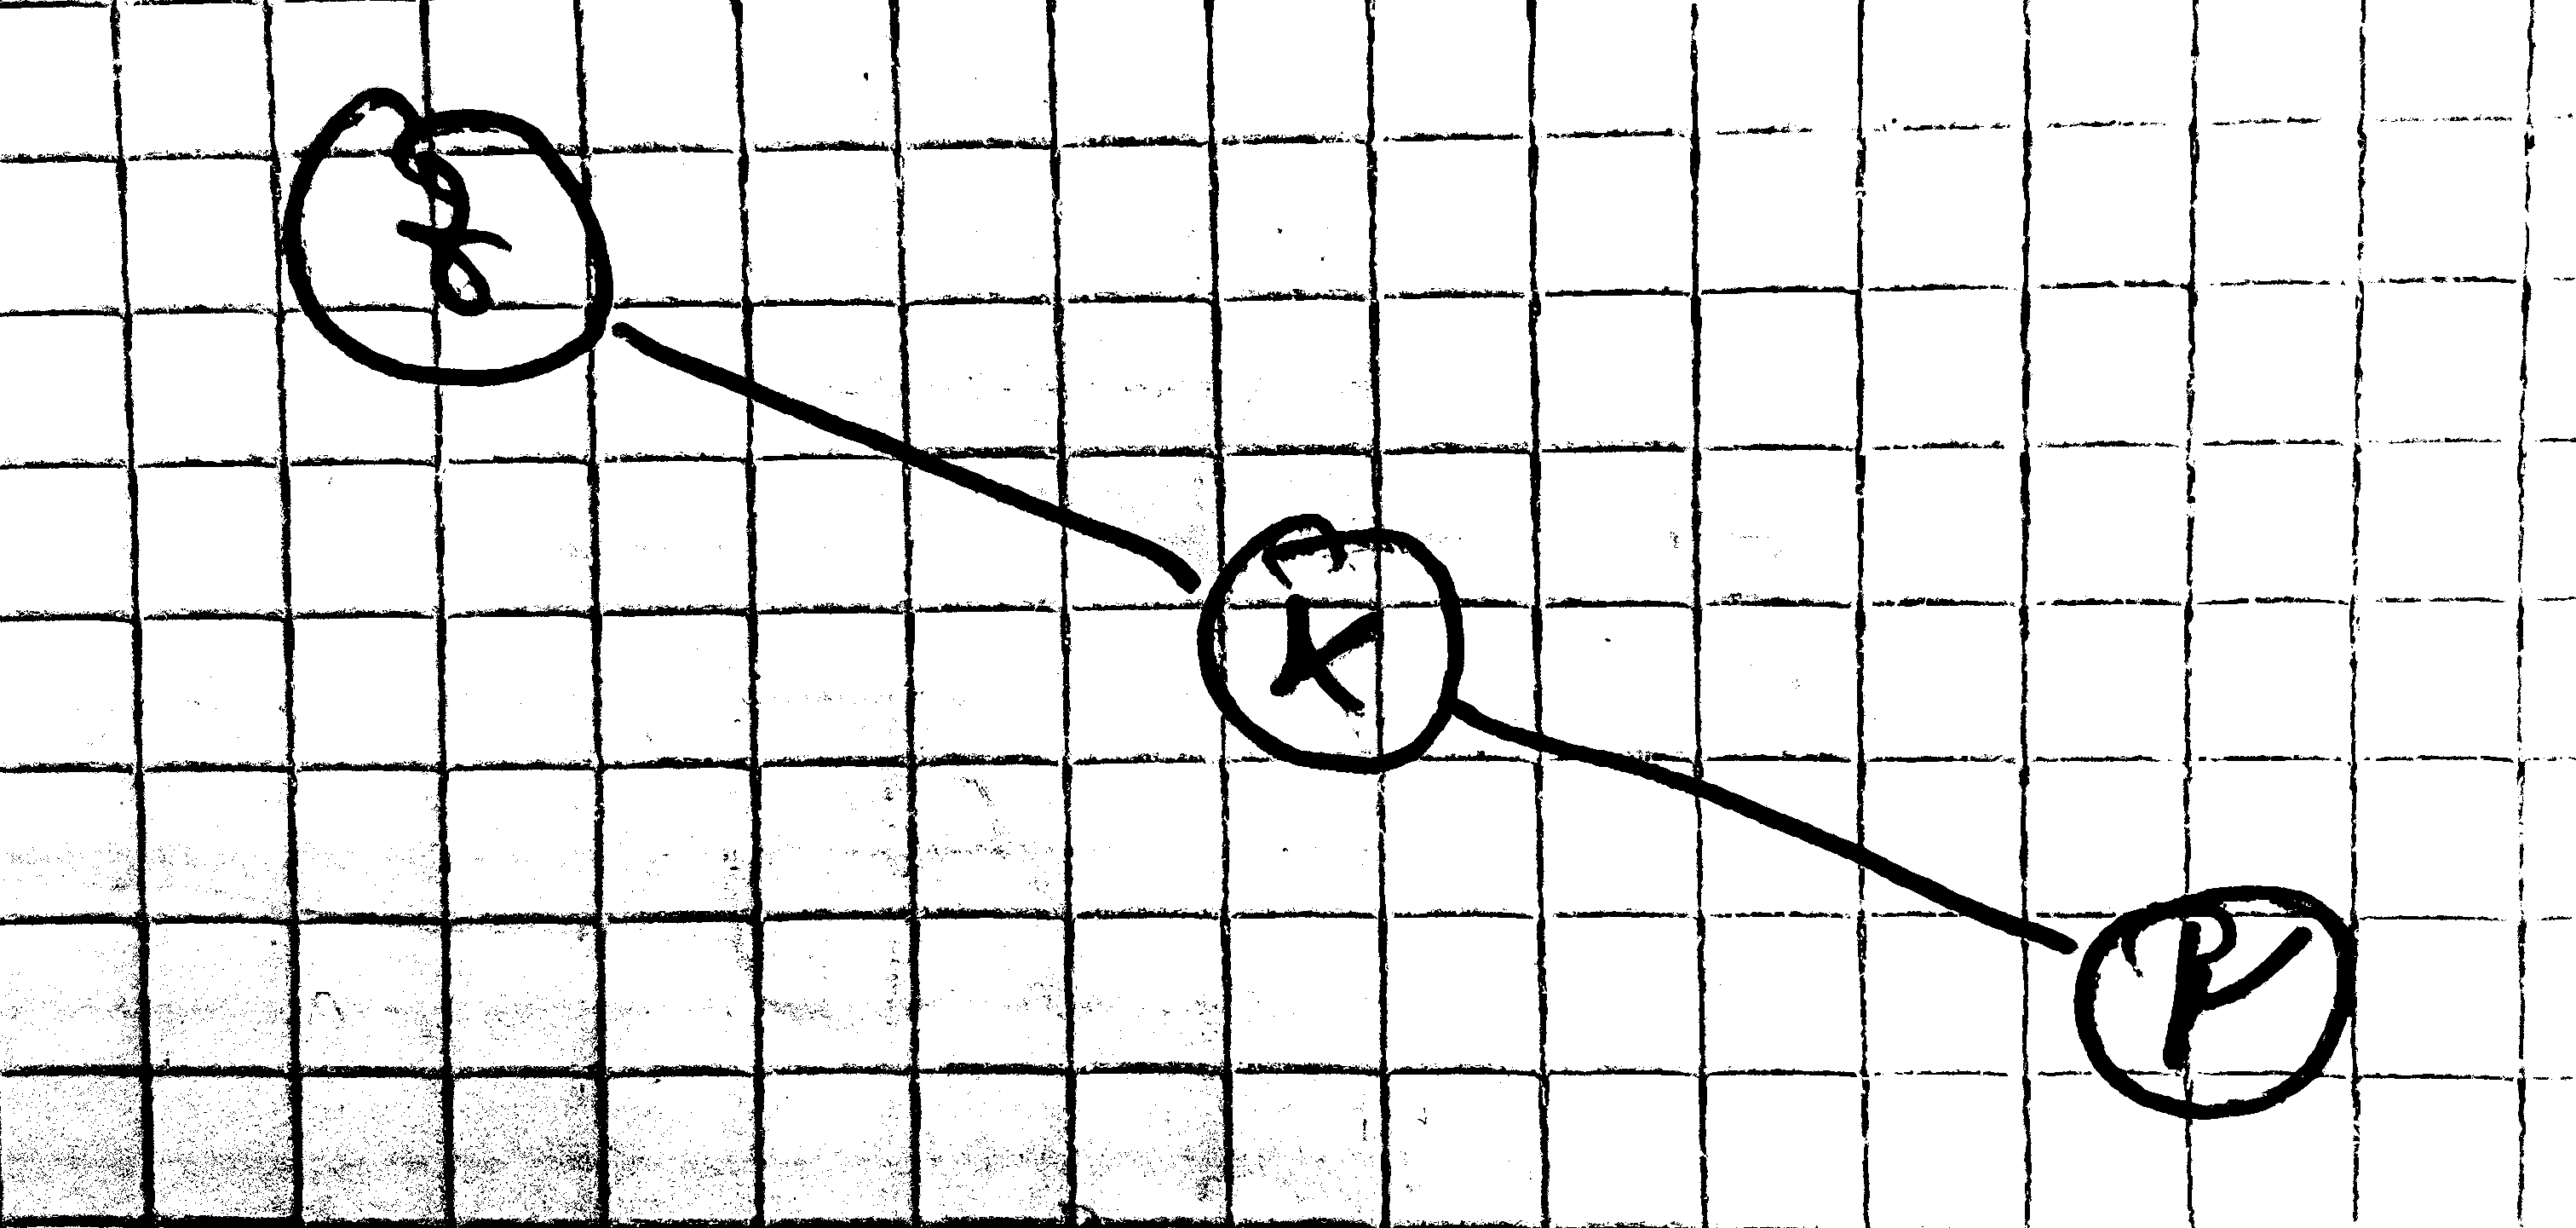
\includegraphics[scale=0.07]{imgs/img18.png}
	\end{center}
	\caption{X is a genuine cause of Y if Z is potential for X, and X blocks the path from Z to Y}
	\label{fig:x_genuine_cause_of_y}
\end{figure}

\define{Spurious association} Two variables $X, Y$ are spuriously associated if they are dependent in some context and there exist two other variables $Z_1, Z_2$ and two contexts $S_1, S_2$:

1. $X \not \independent Z_1 | S_1$

2. $Y \independent Z_1 | S_1$

3. $X \independent Z_2 | S_2$

4. $Y \not \independent Z_2 | S_2$

Conditions 1 and 2 do not allow assigning $X$ as the cause of $Y$: indeed, if there exists an unblocked $S$ path $Z_1 \leadsto X$, then $X$ cannot be the cause of $Y$, as otherwise there would be an unblocked path from $Z_1$ to $Y$ (\ref{fig:x_not_cause_of_y}). Similarly, conditions 3,4 do not allow assigning $Y$ as a potential cause of $X$ (\ref{fig:y_not_cause_of_x}), meaning the only explanation for their association is a common hidden cause.

\begin{figure}[!tbph]
	\centering
	\begin{subfigure}[t]{0.4\textwidth}
		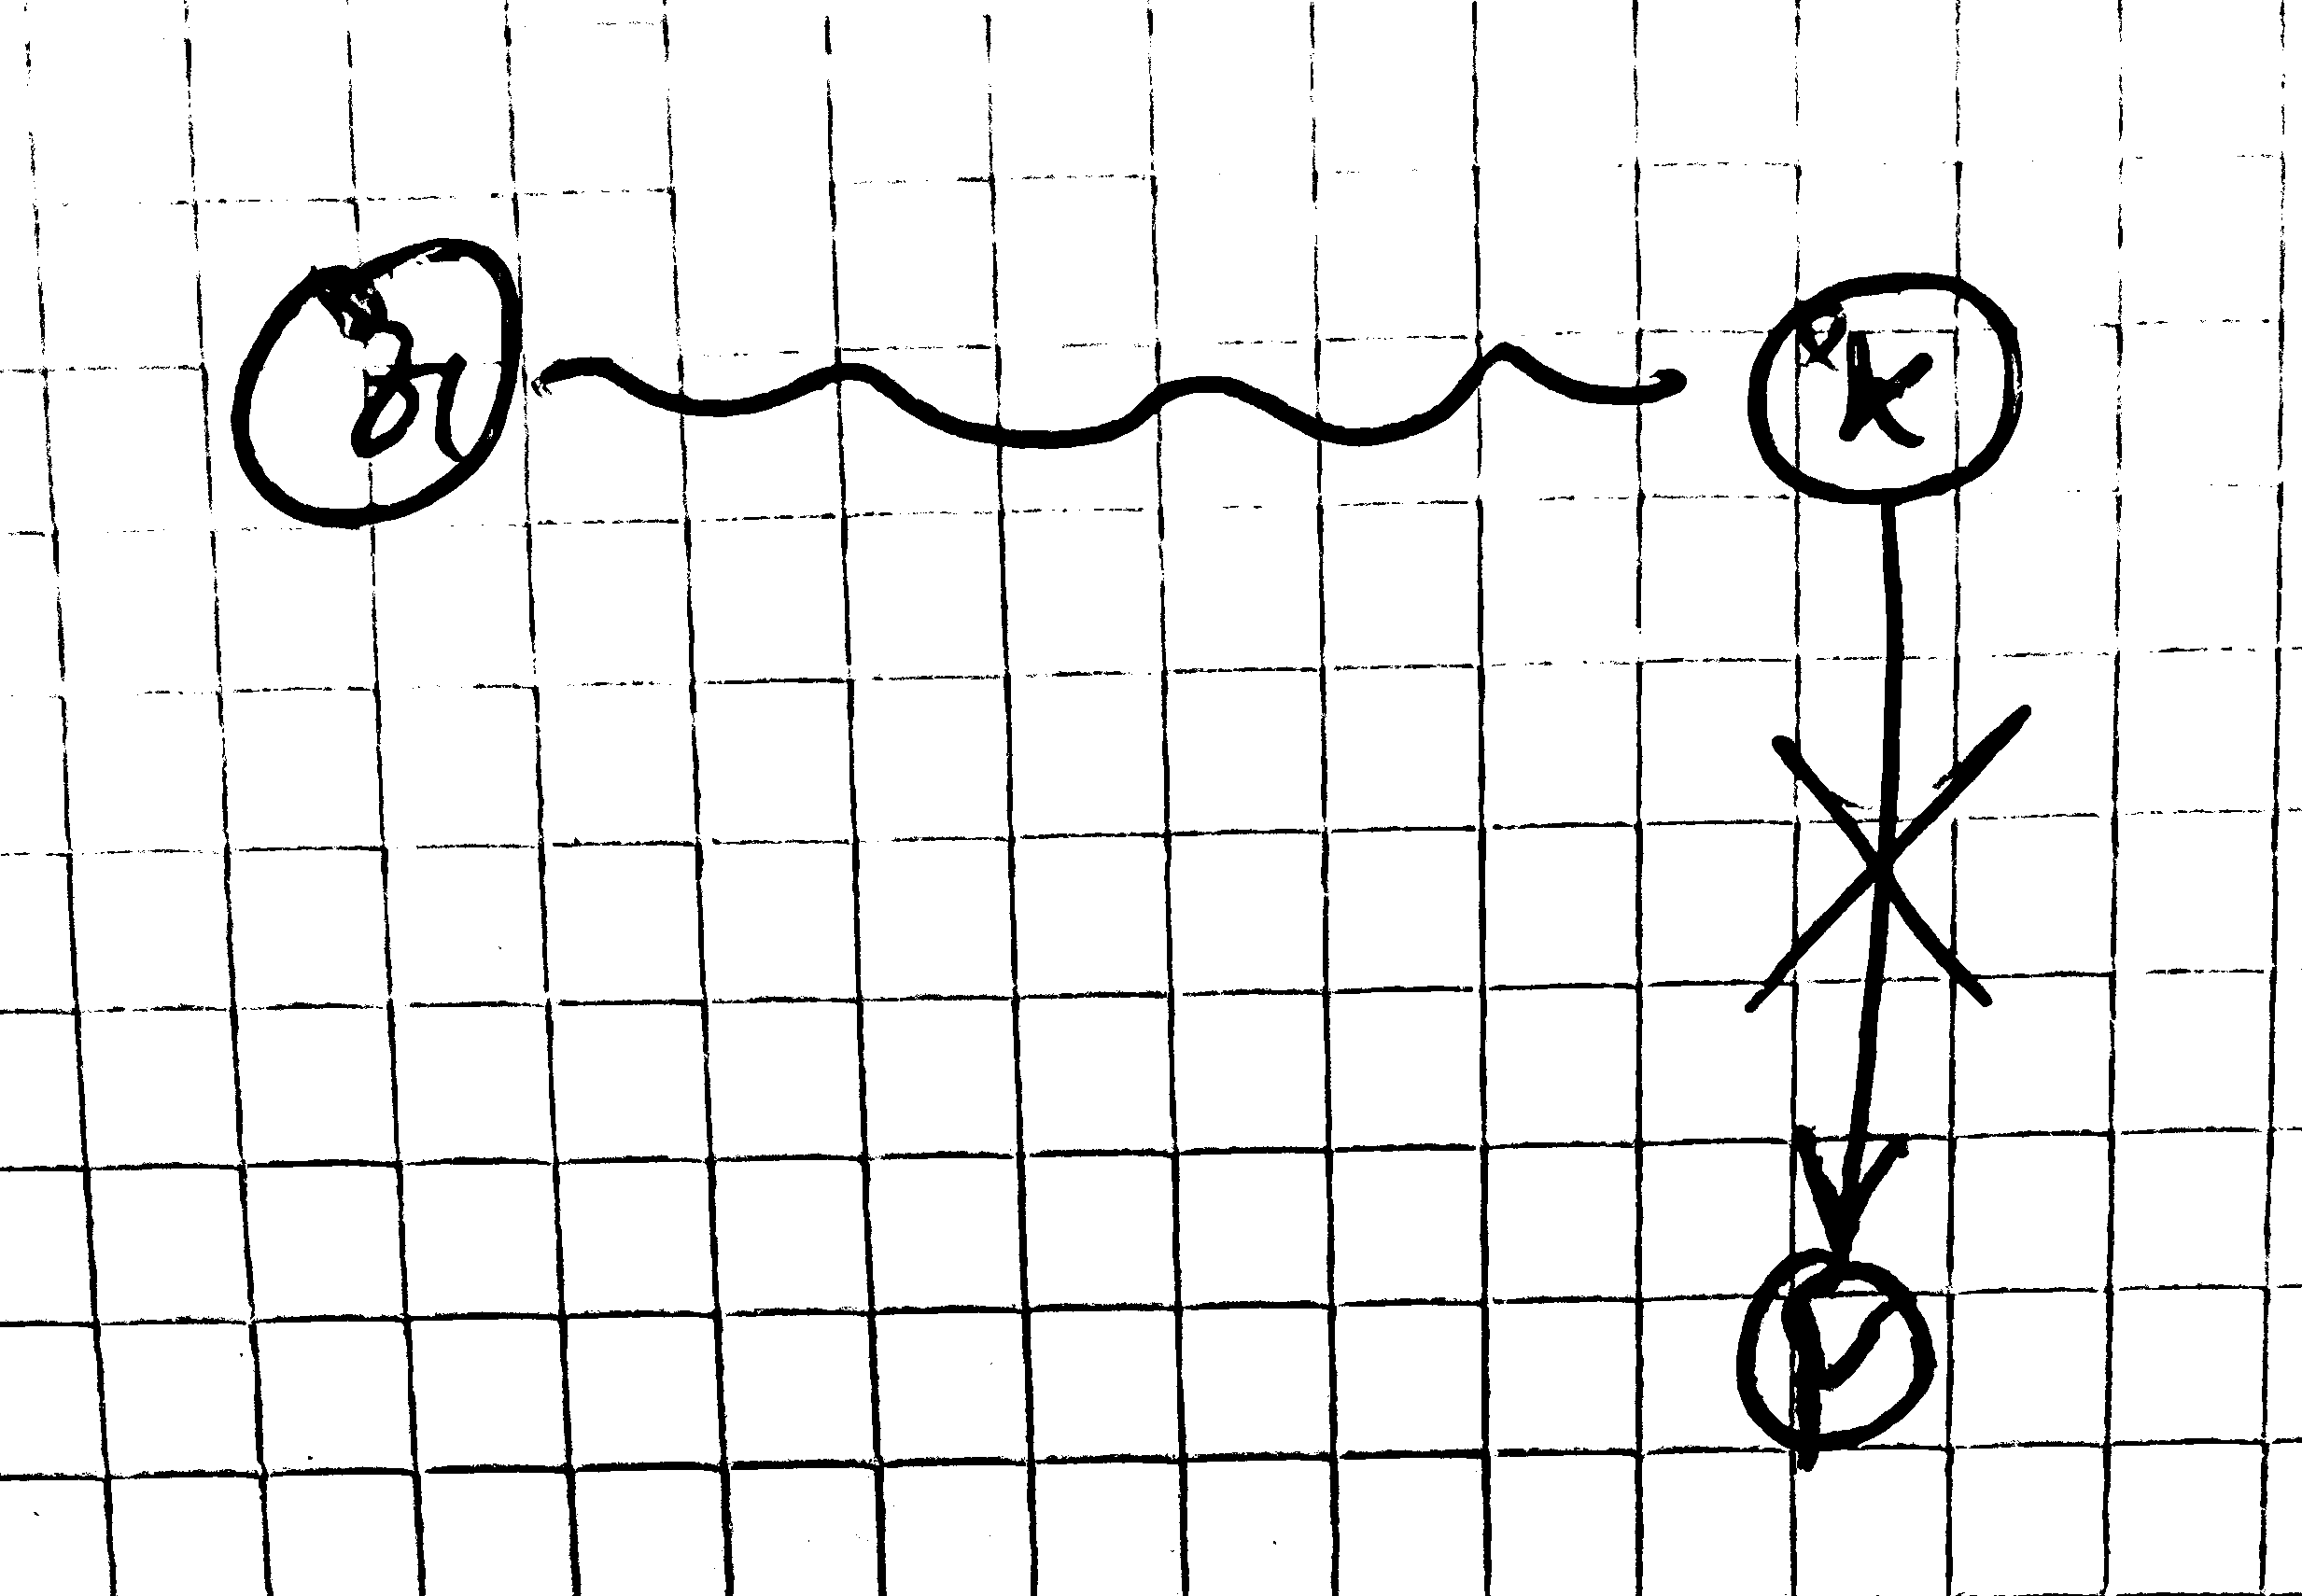
\includegraphics[width=\textwidth]{imgs/img15.png}
		\caption{X cannot be the cause of Y}
		\label{fig:x_not_cause_of_y}
	\end{subfigure}
	\begin{subfigure}[t]{0.4\textwidth}
		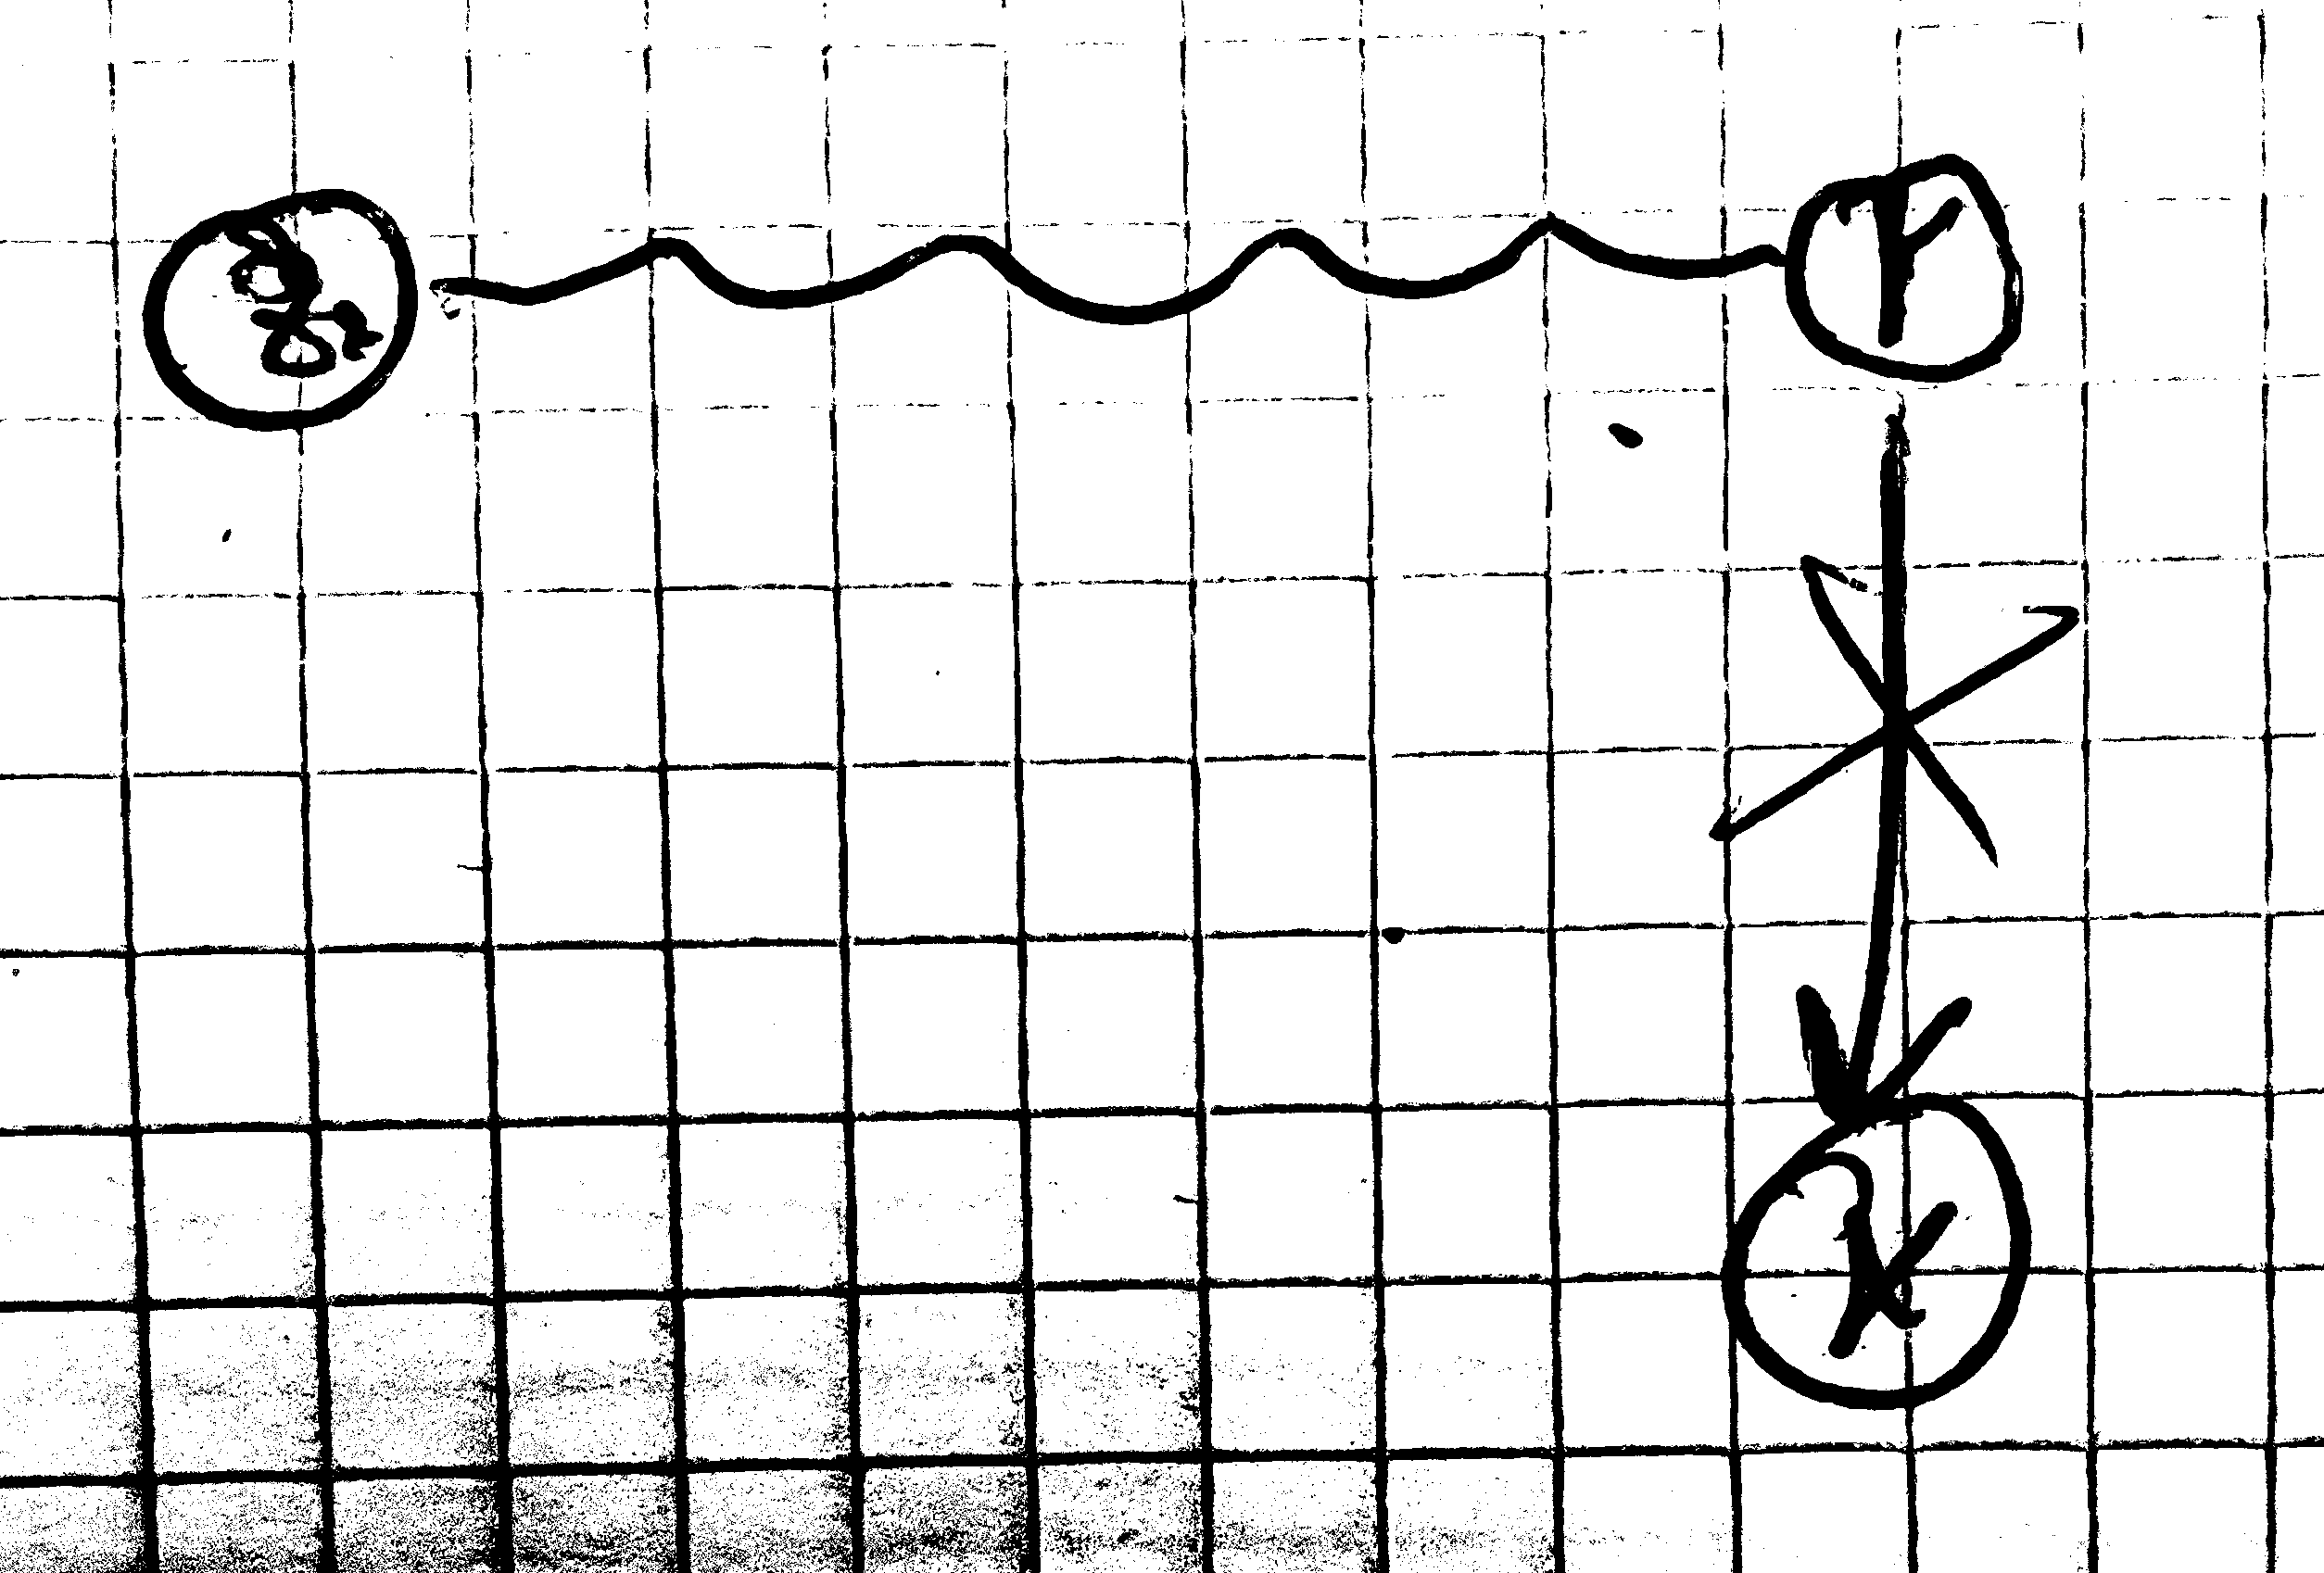
\includegraphics[width=\textwidth]{imgs/img16.png}
		\caption{Y cannot be the cause of X}
		\label{fig:y_not_cause_of_x}
	\end{subfigure}
\end{figure}

When we have temporal information, the definition of causality simplifies: any event that precedes another is its potential cause (since the latter cannot be the cause of the former, as a cause cannot occur after its effect). This leads to more concise definitions.

\define{Genuine cause with temporal information} Variable $X$ has a genuine causal influence on variable $Y$ if there exists a context $S$ and a variable $Z$ occurring before $X$:

1. $Y \not \independent Z | S$

2. $Y \independent Z | S \cup X$

Essentially, this is the same definition of a genuine cause without temporal information, but now to establish potential causality, it's sufficient that $X$ occurred after $Z$.

\define{Spurious association with temporal information} - two variables are spuriously associated if $X$ occurred before $Y$, they are dependent in some context $S$, and there exists a variable $Z$:

1. $Z \independent Y | S$

2. $Z \not \independent X | S$

\section{Causal Diagrams and Establishing Causal Effects}

In the previous chapter, we studied methods for inferring causal relationships from raw data without invoking any additional assumptions. In this section, we will study what conclusions can be drawn from a combination of data and qualitative causal assumptions considered acceptable in a given domain. The main task will be to determine whether the observed data (without the need for experiments) are sufficient to identify certain causal effects.

Causal effects allow us to understand how a system responds to interventions. In this chapter, we will use causal diagrams to describe interventions and define post-intervention distributions through pre-intervention ones. We will show that the effect of any intervention can be calculated from purely observational data provided that the causal diagram contains no unobserved variables and is a DAG.

When not all variables are observed, the question of identifiability of causal relationships and effects arises. This section will present a framework for nonparametric identification of such relationships.

\subsection*{Interventions in Markov Models}

\subsubsection*{Graphs as Models of Interventions}
We previously established that causal models, unlike probabilistic ones, allow computing intervention effects. For this, the joint distribution $P$ must be accompanied by a causal diagram—a DAG defining causal relationships between variables.

The simplest type of intervention is when we set a fixed value $x_i$ for some variable $X_i$. Such an intervention, called atomic, consists of $X_i$ no longer behaving according to the law described by the corresponding functional equation $x_i = f_i(pa_i, u_i)$, but instead behaving according to the law $x_i = x_i$ (here, the left $x_i$ is not a constant but simply denotes the variable; the equality sign is not symmetric in functional equations). Such an intervention is denoted by $do(X_i = x_i)$ or simply $do(x_i)$. In the resulting new model (with the replaced behavior mechanism for $X_i$), if we compute the distribution function for $X_j$, we obtain the causal effect of $X_i$ on $X_j$, denoted $P(x_j | \hat x_i)$.

In the general case, when a set of variables is intervened upon by assigning them fixed values, we remove the corresponding equations for these variables and obtain a new distribution describing the post-intervention world.

\define{Causal effect} Let $X, Y$ be two disjoint sets of variables. The causal effect of $X$ on $Y$, denoted $P(y|\hat x)$ or $P(y | do(x))$, is a function mapping $X$ to the space of probability distributions over $Y$. For any specific realization $X = x$, $p(y|\hat x)$ defines the probability $Y = y$ generated by the post-intervention causal model.

As we previously showed in the section on causal Bayesian networks, the graph corresponding to the truncated set of equations is a subgraph of the original graph where all incoming edges to the intervened variables are removed.

\subsubsection*{Interventions as Variables}

In some cases, it is convenient to consider the perturbation describing an intervention also as a variable in the graph: that is, to view $f_i$ as an instance of variable $F_i$ and write the structural equation as:

\begin{align}
	\begin{split}
		x_i &= I(pa_i, f_i, u_i)
	\end{split}
\end{align}

Here, I is some three-place function satisfying the condition $I(a,b,c) \equiv f_i(a,c)$ if $b = f_i$.

The diagram corresponding to this interpretation of the intervention contains a new edge compared to the original graph:

\begin{figure}[h]
	\begin{center}
		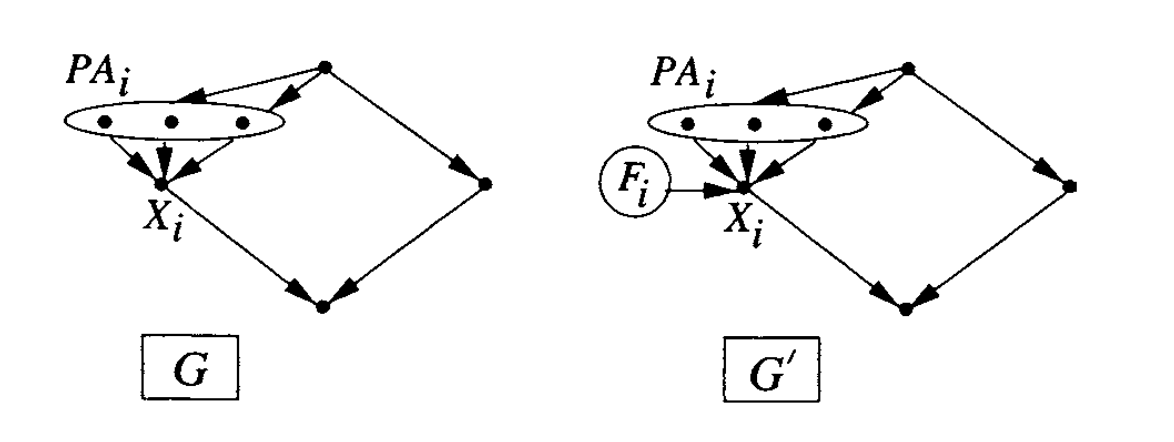
\includegraphics[scale=0.6]{imgs/img19.png}
	\end{center}
	\caption{Representation of intervention through an extended diagram}
	\label{fig:explicit_intervention_in_graph}
\end{figure}

\subsubsection*{Computing the Effect of an Intervention}

Consider an atomic intervention $do(X_i = x_i')$. It defines the distribution $P(x_1,..,x_n|\hat x_i') = \prod\limits_{j\neq i}P(x_j | pa_j)$, when $x_i = x_i'$, and equal to 0 in all other cases. Divide and multiply this equality by $P(x_i | pa_i)$, and obtain:

\begin{align}
	P(x_1,...,x_n|\hat x_i') = \begin{cases}
		\frac{P(x_1,...,x_n)}{P(x_i | pa_i)} & \ x_i = x_i'\\
		0 & \ x_i \neq x_i'
	\end{cases}
	\label{eq:intervention}
\end{align}

This equality is interesting from the perspective of mass redistribution: under the intervention, the mass (probability measure) of the point $(x_1, ..., x_n)$ increases by $\frac{1}{P(x_i' | pa_i)}$. Thus, for points where the conditional probability $P(x_i'|pa_i)$ is small, the probability substantially increases under the intervention, while points where $X_i = x_i'$ is quite natural ($P(x_i'|pa_i) \approx 1$) do not change their mass much.

In the ordinary Bayesian approach, the excluded points $x_i \neq x_i'$ transfer their mass to all other points via the normalization constant $\frac{1}{P(x_i')}$. In our case, a different transformation occurs: the mass of a point is distributed among points sharing the same $pa_i$. Indeed: $P(pa_i | do(x_i')) = P(pa_i)$—meaning the total mass distributed over $pa_i$ is preserved, so the mass of each point $X = (s_i, x_i, pa_i)$, where $s_i = instance(S)$, $S = V \backslash (PA_i \cup \{X_i\})$ is somehow distributed among points with the same $pa_i$ and $x_i = x_i'$. The factor by which the mass of each point increases for a given $pa_i$ is the same—$\frac{1}{P(x_i'|pa_i)}$.

We can look at equality \ref{eq:intervention} differently:

\begin{align}
	P(x_1,...,x_n|\hat x_i') = \begin{cases}
		P(x_1,...,x_n| x_i, pa_i)P(pa_i) & \ x_i = x_i'\\
		0 & \ x_i \neq x_i'
	\end{cases}
	\label{eq:intervention2}
\end{align}

\begin{theorem}
	\textbf{Accounting for Immediate Causes} Let $PA_i$ be the set of immediate causes of variable $X_i$ and $Y \cap \{PA_i \cup X_i\} = \emptyset$. Then the effect of intervention $do(X_i = x_i')$ on $Y$ is computed by the formula:
	\begin{align}
		P(y|\hat x_i') = \sum\limits_{pa_i} P(y|x_i', pa_i) P(pa_i)
		\label{eq:adjusting_formula}
	\end{align}
\end{theorem}

The theorem follows directly from summing formula \ref{eq:intervention2} over all variables except $Y$ $\blacksquare$.

The operation consisting of such conditioning followed by averaging the result, weighted by the prior probabilities $pa_i$, is called "adjusting for $PA_i$."

In the more general case, when the intervention consists of setting some subset of variables $S$ to constants $do(S = s)$, we obtain a similar formula for the post-intervention distribution:

\begin{align}
	P(x_1,...,x_n|\hat s) = \begin{cases}
		\prod\limits_{i| X_i \notin S} P(x_i|pa_i) & x_1,...,x_n \text{ consistent with } s\\
		0 & \text{otherwise}
	\end{cases}
	\label{eq:intervention3}
\end{align}

We can go even further and consider an arbitrary intervention that replaces some causal mechanisms with new ones. For example, if we replace the mechanism defining $X_i$: $P(x_i|pa_i) \leadsto P^*(x_i | pa^*_i)$ (the set of causes of variable $X_i$ may also change), then the resulting distribution after the intervention will be:

\begin{align}
	P^*(x_1,..,x_n) = P(x_1,...,x_n) \frac{P^*(x_i|pa^*_i)}{P(x_i|pa_i)}
\end{align}

Conclusions: given a causal diagram where all immediate causes of the variables being intervened upon are observed, we can determine the post-intervention distribution from the pre-intervention one using the truncated factorization formula \ref{eq:intervention3}.

Generally speaking, the more interesting situation is when not all direct causes are observed, which prevents direct determination of $P(x_i' | pa_i)$. Next, graphical methods for checking whether $P(x_j|\hat x_i')$ can be estimated will be developed, but first, let's formally define what it means for a causal quantity Q to be estimable from passive observations—the possibility of \textit{identification}.

\subsubsection*{Identification of Causal Quantities}

Causal quantities, unlike statistical parameters, are defined relative to a causal model $M$, not just the joint distribution $P_M(v)$ over the set of observed variables. Since non-experimental data only provide information about $P_M(v)$, and since multiple models can generally generate the same distribution, it is possible that the quantity of interest may not be uniquely determined by the available data, regardless of the sample size. Identifiability ensures that additional assumptions about the causal model (e.g., causal structure or zero coefficients in structural equations) provide the necessary additional information without requiring the full specification of model $M$.

\define{Identifiability} Let $Q(M)$ be any computable quantity in model $M$. We say that $Q(M)$ is identifiable in the class of models \textbf{M} if for any two models in this class, $M_1$ and $M_2$, the equality $P_{M_1}(v) = P_{M_2}(v)$ implies $Q(M_1) = Q(M_2)$. If our observations are limited and we only know some set of features $F_M$ of the distribution $P_M(v)$, then we say that $Q(M)$ is identifiable given $F_M$ if $F_{M_1} = F_{M_2}$ implies $Q(M_1) = Q(M_2)$.

Identifiability is necessary to combine statistical data with incomplete causal knowledge $\{f_i\}$, as it allows consistent estimation of quantities $Q$ from large samples $P(v)$ without detailed specification of $M$: some general characteristics of the model class \textbf{M} are sufficient. Currently, the causal quantity $Q$ of interest to us is the causal effect $P_M(y | \hat x)$, which is computable given a model $M$ (using its definition), but usually, we need to compute it without a full specification of $M$.

We will consider the following class \textbf{M} of causal models, within which we will define identifiability:

1. Models share a common causal structure.

2. Define positive distributions over the set of observed variables $v$: $P(v) > 0$.

\define{Identifiability of Causal Effect} The causal effect of $X$ on $Y$ is identifiable from graph $G$ if the quantity $P(y|\hat x)$ can be uniquely computed from any positive distribution of observed variables, i.e., if $P_{M_1}(y|\hat x) = P_{M_2}(y|\hat x)$ for any pair of models $M_1, M_2$ for which $P_{M_1}(v) = P_{M_2}(v)$ and whose graphs coincide.

Identifiability of $P(y|\hat x)$ guarantees that the causal effect $do(X = x)$ on $Y$ can be computed from two sources of data:

1. Passive observations allowing reconstruction of $P(v)$.

2. The causal graph $G$, which qualitatively determines which variables define stable causal mechanisms (which variables determine other variables).

Positivity of the distribution ensures that in formula \ref{eq:intervention}, we do not divide by 0: logically, if the probability of observing $x_i'$ in the context of $pa_i$ were zero, we could not infer the effect of the action $do(X_i=x_i')$.

Note that to establish non-identifiability, it is sufficient to provide as an example two sets of structural equations that define the same distributions over observed variables but have different causal effects.

\begin{theorem}
	Given a causal diagram $G$ of a Markov model in which some subset $V$ of variables is observed, the causal effect $P(y|\hat x)$ is identifiable if $\{X \cup Y \cup PA_x\} \subset V$. The expression for $P(y|\hat x)$ in this case is determined by accounting for direct causes using formula \ref{eq:adjusting_formula}.
\end{theorem}

\subsection*{Controlling Confounding Bias}

When we want to estimate the effect of some factor $X$ on another $Y$, the question arises whether we need to standardize measurements for various values of other factors $Z$, also known as covariates/confounders. Standardization involves splitting the population into subgroups homogeneous with respect to $Z$, estimating the effect in each subgroup, and averaging the result.

The illusory nature of standardization was discovered by Pearson in 1899 when he observed Simpson's paradox: any statistical relationship between two variables can be inverted by including additional factors in the analysis. Thus, the question arises: which variables should we account for to avoid confounding?

\subsubsection*{Backdoor Criterion}

\define{Backdoor Criterion} A set of variables $Z$ satisfies the backdoor criterion relative to an ordered pair of variables $(X_i, X_j)$ in DAG $G$ if:

1. No vertex in $Z$ is a descendant of $X_i$.

2. $Z$ blocks every path between $X_i$ and $X_j$ that contains an edge directed into $X_i$.

In the general case, when there are two sets of variables $X, Y$, we say that $Z$ satisfies the backdoor criterion if it satisfies it for any ordered pair $(X_i, X_j): X_i \in X, X_j \in Y$.

\begin{theorem}
	\textbf{Backdoor Adjustment} If a set of variables $Z$ satisfies the backdoor criterion relative to $(X,Y)$, then the causal effect is identifiable and is given by the formula:
	
	\begin{align}
		P(y|\hat x) = \sum\limits_{z} P(y|x, z) P(z)
	\end{align}
\end{theorem}

Proof of the theorem. For the proof, it is most convenient to consider an extended graph that includes vertices representing causal mechanisms. Since all backdoor paths are blocked by $Z$, any path $F_x \leadsto Y$ goes through children of $X$, but these paths are blocked when conditioning on $X$. Thus, we conclude that $Y$ is independent of $F_x$ given $X, Z$:

\begin{align}
	P(y|x, z, F_x = do(x)) = P(y | x, z, F_x = idle) = P(y|x, z)
	\label{eq:backdoor1}
\end{align}
which means that observing $X=x$ is indistinguishable in the context of $Z$ from the intervention $do(X = x)$.

Indeed, if $P'$ is the distribution generated by the extended graph $G'$, then:

\begin{align}
	P(y|\hat x) = P'(y|F_x) = \sum\limits_{z}P'(y|z, F_x)P'(z|F_x) = \sum\limits_{z}P'(y|z, x, F_x)P'(z|F_x)
\end{align}

The last equality holds because $F_x \implies X = x$. Now we need to eliminate the two $F_x$ terms on the right side of the equality. Note that $F_x$ are root vertices in $G'$, with children $X$. Therefore, $F_x \independent Z | X$, as they are $d$-separated, since $Z$ are not descendants of $X$ by the first condition of the backdoor criterion. Thus:

\begin{align}
	P'(z|F_x) = P'(z) = P(z)
\end{align}

As for $P'(y|z, x, F_x)$, according to \ref{eq:backdoor1}, it is equivalent to $P(y|x,z)$. Ultimately, we obtain exactly what was required. $\blacksquare$

\subsubsection*{Front-Door Criterion}

Consider the following diagram:
\begin{figure}[h]
	\begin{center}
		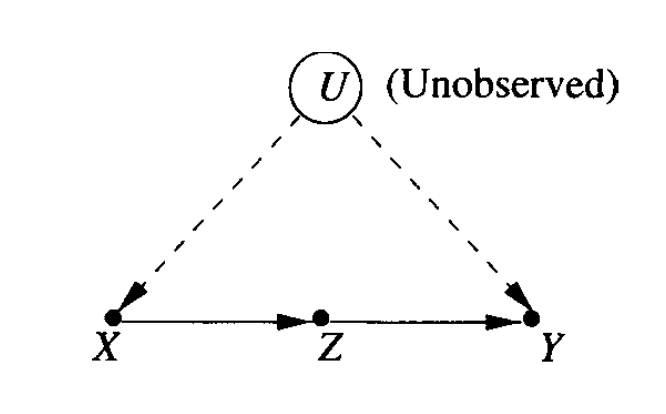
\includegraphics[scale=0.6]{imgs/img20.png}
	\end{center}
	\caption{Diagram illustrating the front-door criterion}
	\label{fig:frontdoor1}
\end{figure}

The distribution corresponding to the diagram factorizes as:

\begin{align}
	P(x,z,y,u) = P(u)P(x|u)P(z|x)P(y|z,u)
\end{align}

The intervention $X=do(x)$ leads us to a factorization without the factor for $X$:

\begin{align}
	P(z,y,u|\hat x) = P(u)P(z|x)P(y|z,u)
\end{align}

Summing over $u,z$ to compute the effect on $y$:

\begin{align}
	P(y|\hat x) = \sum\limits_{z}P(z|x)\sum\limits_{u}P(u)P(y|z,u)
	\label{eq:frontdoor2}
\end{align}

This cannot be used directly because $u$ is unobserved—we need to eliminate it somehow.

Note that by $d$-separation in the graph, we have the following independencies:

\begin{align}
	P(u|z,x) = P(u|x)\label{eq:frontdoor_cond1}\\
	P(y|z,u,x) = P(y|u,z)
	\label{eq:frontdoor_cond2}
\end{align}

Using these equalities, consider component \ref{eq:frontdoor2}:
\begin{align}
	\begin{split}
		\sum\limits_{u}P(u)P(y|z,u) &= \sum\limits_{x} \sum\limits_{u}P(u|x)P(x)P(y|z,u)\\ 
		&= \sum\limits_{x} \sum\limits_{u}P(u|x,z)P(x)P(y|z,u,x) \\
		&= \sum\limits_{x} \sum\limits_{u}P(y,u|z,x)P(x) \\
		&= \sum\limits_{x} P(y|z,x)P(x)
	\end{split}
	\label{eq:frontdoor3}
\end{align}

which allows us to transform \ref{eq:frontdoor2} into:
\begin{align}
	P(y|\hat x) = \sum\limits_{z}P(z|x) \sum\limits_{x} P(y|z,x)P(x)
	\label{eq:frontdoor4}
\end{align}

In this formula, all factors on the right side can be estimated from observed data, implying that $P(y|\hat x)$ can also be estimated. Thus, under the conditions \ref{eq:frontdoor_cond1}, \ref{eq:frontdoor_cond2}, we can unbiasedly estimate the effect of $X$ on $Y$.

Formula \ref{eq:frontdoor4} can be interpreted as a two-step application of backdoor adjustment: first, we compute the effect of $X$ on $Z$: since there are no unblocked backdoor paths from $Z$ to $X$, then:

\begin{align}
	P(z|\hat x) = P(z|x)
\end{align}

Then, we compute the effect of $Z$ on $Y$. Here, we have an unblocked backdoor path $Y \leftarrow U \rightarrow X \rightarrow Z$, which can be blocked by conditioning on $X$, so $X$ satisfies the backdoor criterion in this case, and thus:

\begin{align}
	P(y|\hat z) = \sum\limits_{x'}P(y|z,x')P(x')
\end{align}

Finally, we combine the two causal effects to obtain:
\begin{align}
	P(y|\hat x) = \sum\limits_{z}P(z|\hat x) P(y|\hat z)
\end{align}

\define{Front-Door Criterion}
A set of variables $Z$ satisfies the front-door criterion relative to an ordered pair of variables $(X, Y)$ if:

1. $Z$ blocks all directed paths $X \leadsto Y$.

2. There are no unblocked backdoor paths $Z \leadsto X$.

3. All backdoor paths $Y \leadsto Z$ are blocked by $X$.

\begin{theorem}
	\textbf{Front-Door Adjustment} If $Z$ satisfies the front-door criterion relative to $(X, Y)$ and $P(x,z) > 0$, then the causal effect of $X$ on $Y$ is identifiable and can be computed as:
	\begin{align}
		P(y|\hat x) = \sum\limits_{z}P(z|x) \sum\limits_{x'}P(y|z,x')P(x')
	\end{align}
\end{theorem}

\subsection*{Calculus of Interventions}
\subsubsection*{Notation}
Let $X, Y, Z$ be disjoint sets of variables. Denote by $G_{\overline{X}}$ the graph obtained by removing from $G$ all edges pointing to $X$. Similarly, denote by $G_{\underline{X}}$ the graph obtained from $G$ by removing all edges originating from $X$. The expression $P(y|\hat x, z) \equiv \frac{P(y, z | \hat x)}{P(z | \hat x)}$ describes the probability $Y=y$ given that we set $X=x$ and observed $Z=z$.

\subsubsection*{Inference Rules}

\begin{theorem}
	\textbf{Do-Calculus Rules} Let $G$ be a DAG with a given causal model, and $P$ the distribution induced by it. For any disjoint sets $X, Y, Z, W$ of variables, the following rules hold:
	
	1. Insertion/Deletion of Observations:
	\begin{align}
		P(y|\hat x, z, w) = P(y|\hat x, w) & \text{ if } Y \independent_{G_{\overline{X}}} Z | X, W
	\end{align}
	
	2. Action/Observation Exchange:
	\begin{align}
		P(y|\hat x, \hat z, w) = P(y|\hat x, z, w) & \text{ if } Y \independent_{G_{\overline{X}\underline{Z}}} Z | X, W
	\end{align}
	
	3. Insertion/Deletion of Actions:
	\begin{align}
		P(y|\hat x, \hat z, w) = P(y|\hat x, w) & \text{ if } Y \independent_{G_{\overline{X}\overline{Z(W)}}} Z | X, W
	\end{align}
	Where $Z(W) \subset Z: de(Z(W)) \cap W = \emptyset$ in $G_{\overline{X}}$
\end{theorem}

The first rule states that $d$-separation is a valid test for independence in the post-intervention distribution: indeed, removing structural equations as a result of intervention does not introduce new dependencies.

The second rule describes the condition under which an external observation $z$ coincides with an intervention: for this to hold, the backdoor criterion must be satisfied: any backdoor path from $Y$ to $Z$ must be blocked, and this is precisely the condition for applying this rule: in $G_{\overline{X}\underline{Z}}$, only backdoor paths from $Y$ to $Z$ exist (since all edges originating from $Z$ are removed by definition in this graph), and if in such a graph $Y \independent Z |W, X$, then $W, X$ block all backdoor paths.

The third rule is the most subtle of the three. To prove it, consider the extended graph $G'$, where vertices $F_z$ and edges $F_z \rightarrow Z$ are added.

Consider two cases—when $Z_i \in Z(W)$ and when $Z_i \notin Z(W)$.

In the first case, we have the situation shown in Figure \ref{fig:rule3}. In $G_{\overline{X},\overline{Z(W)}}$, front-door paths $Z_i \leadsto Y$ coincide with paths in graph $G_{\overline{X}}$, and if in the first graph they are blocked by $W, X$, then in the second (original) graph, they are also blocked. This means that any path $F_{Z_i} \leadsto Y$ passing through an edge from $Z_i$ is blocked. Paths from $F_{Z_i}$ that are backdoor paths relative to $Z_i$ (contain an edge leading to $Z_i$) are blocked by $Z_i$ itself, as they form a $v$-structure.

\begin{figure}[h]
	\begin{center}
		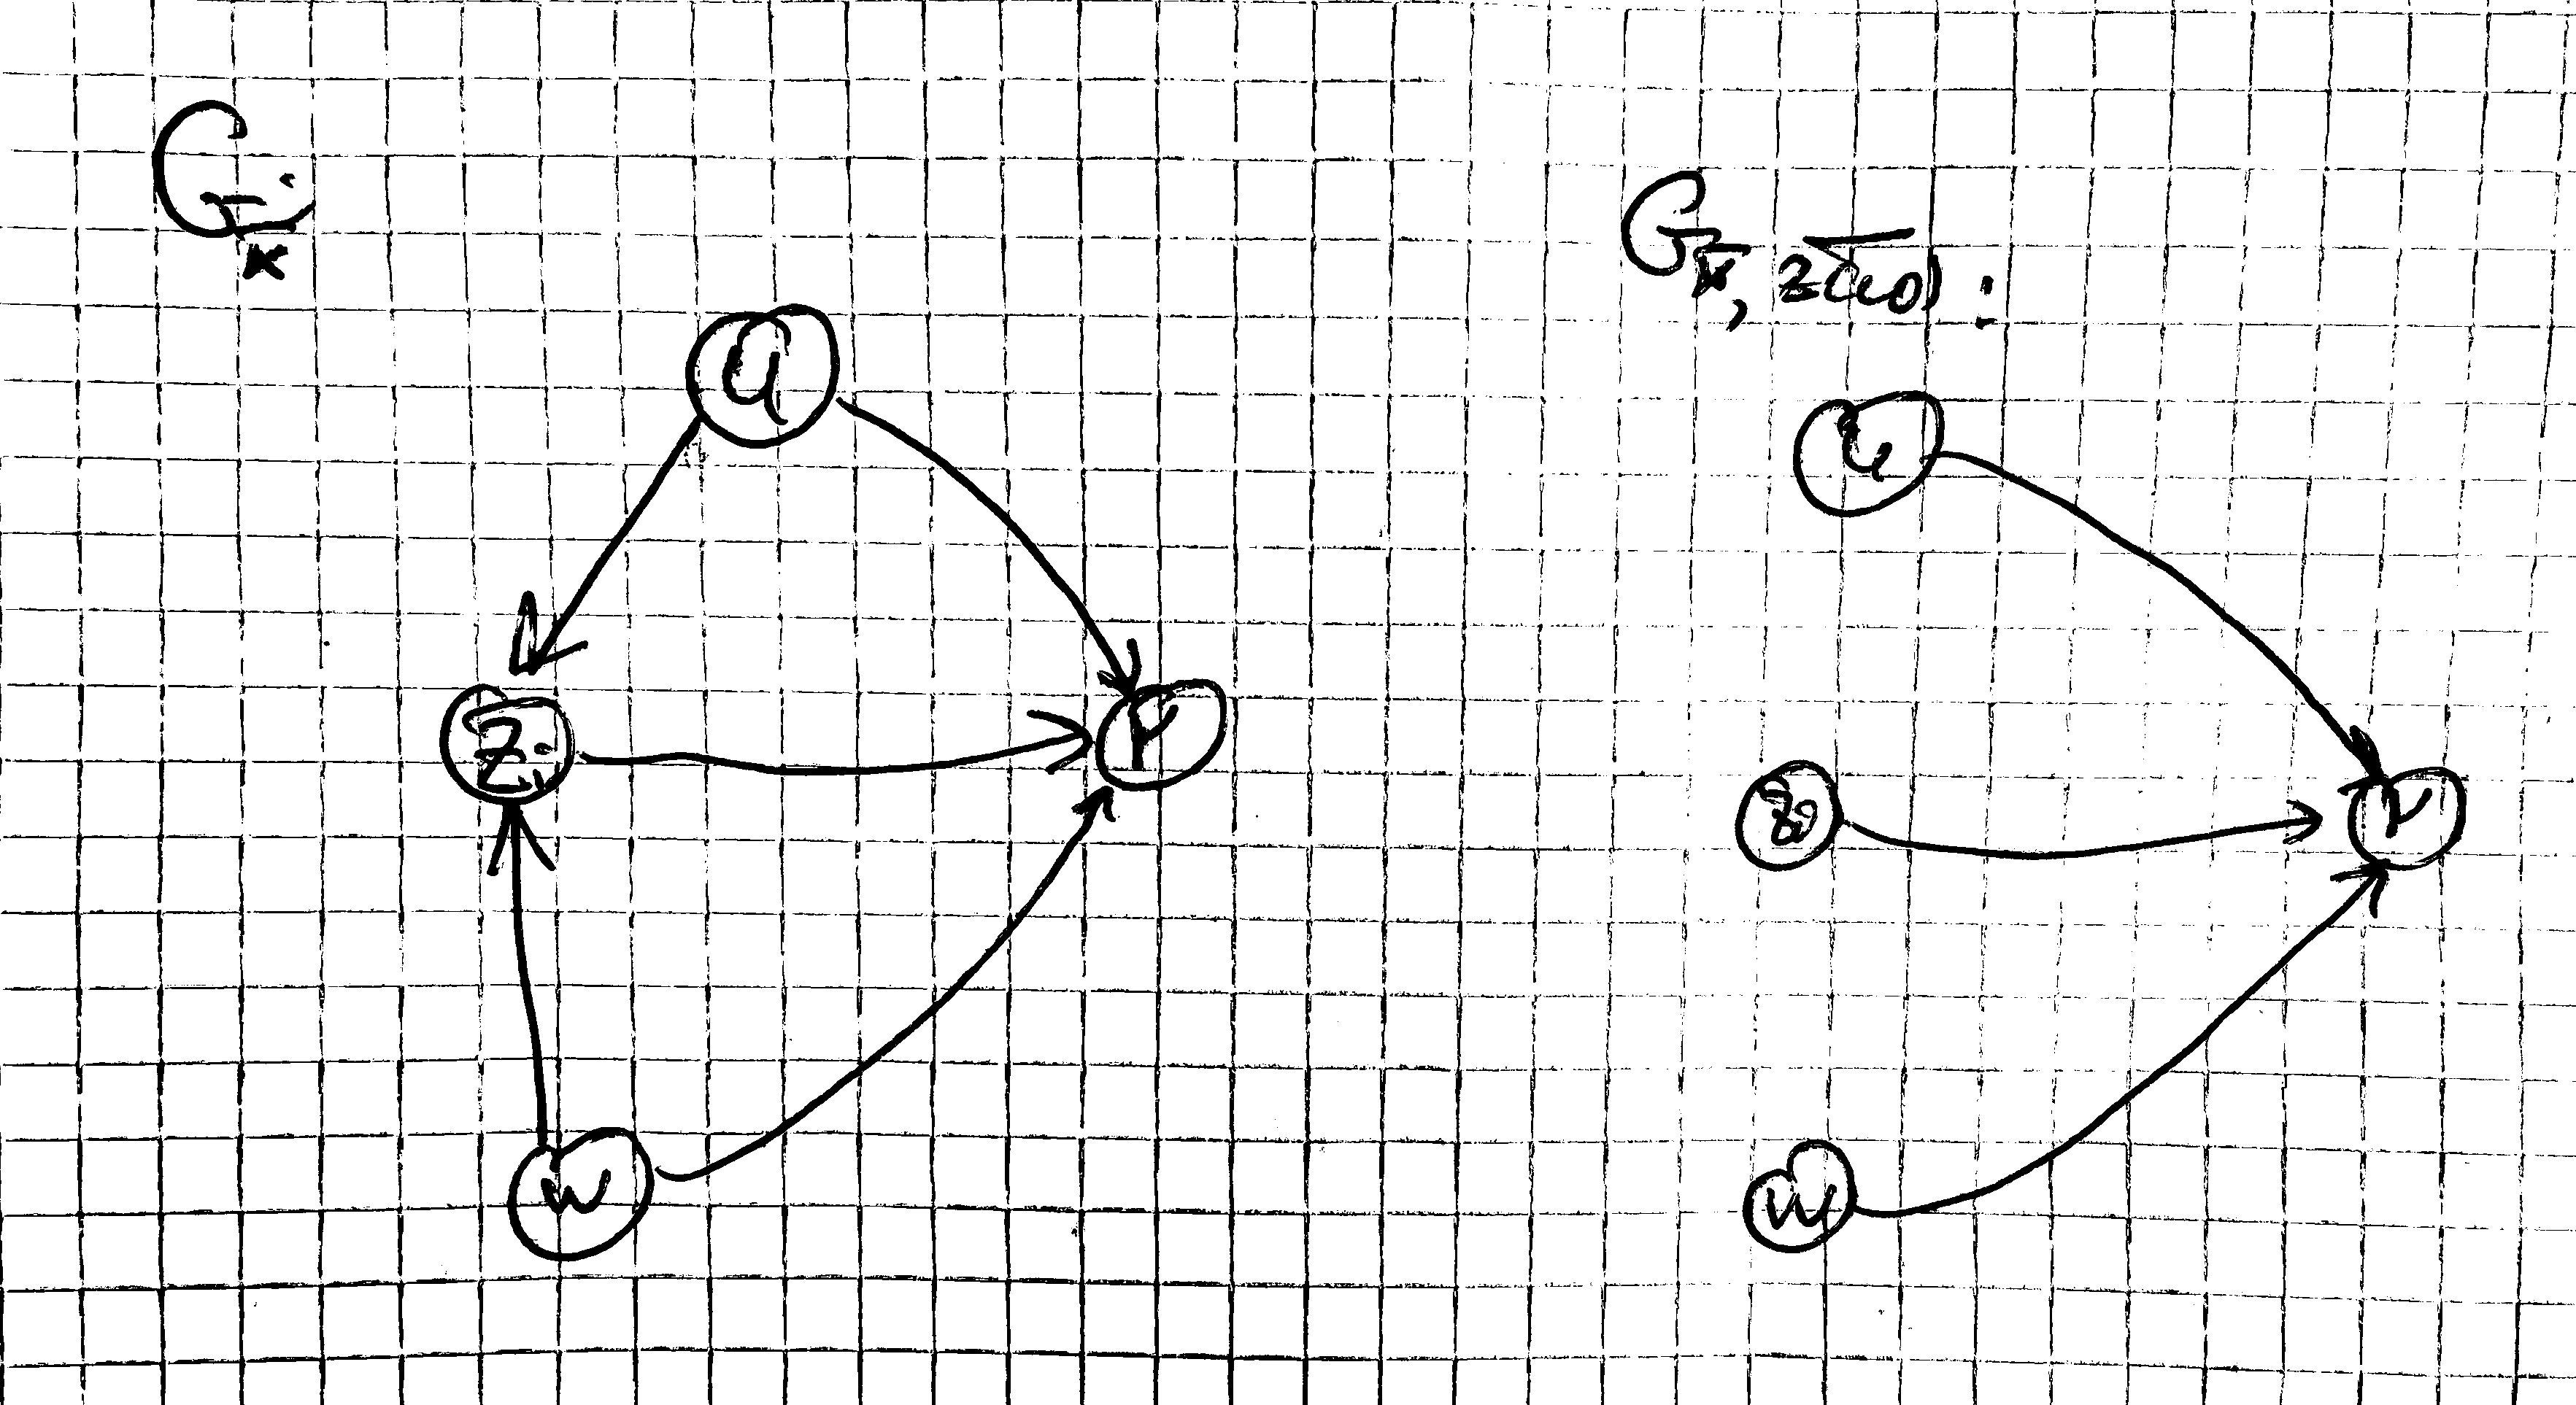
\includegraphics[scale=0.1]{imgs/img21.png}
	\end{center}
	\caption{$Z_i \in Z(W)$}
	\label{fig:rule3}
\end{figure}

In the second case, we have Figure \ref{fig:rule3_2}. In graph $G_{\overline{X},\overline{Z(W)}}$, no edges incident to $Z_i$ are removed, so from the fact that in the manipulated graph $Z$ and $Y$ are $d$-separated by $X,W$, it follows that in the original graph, they are also $d$-separated, meaning $F_z$ is also $d$-separated from $Y$, which was to be shown. $\blacksquare$.

Why do we consider the unmanipulated graph in this case? Actually, because from the statement about the manipulated graph, we cannot derive the statement for the original graph: the path $F_z -\rightarrow Z_i \leftarrow U \rightarrow Y$ would be unblocked, despite not conditioning on $Z_i$, because we are conditioning on descendants of $Z_i$.

\begin{figure}[h!]
	\begin{center}
		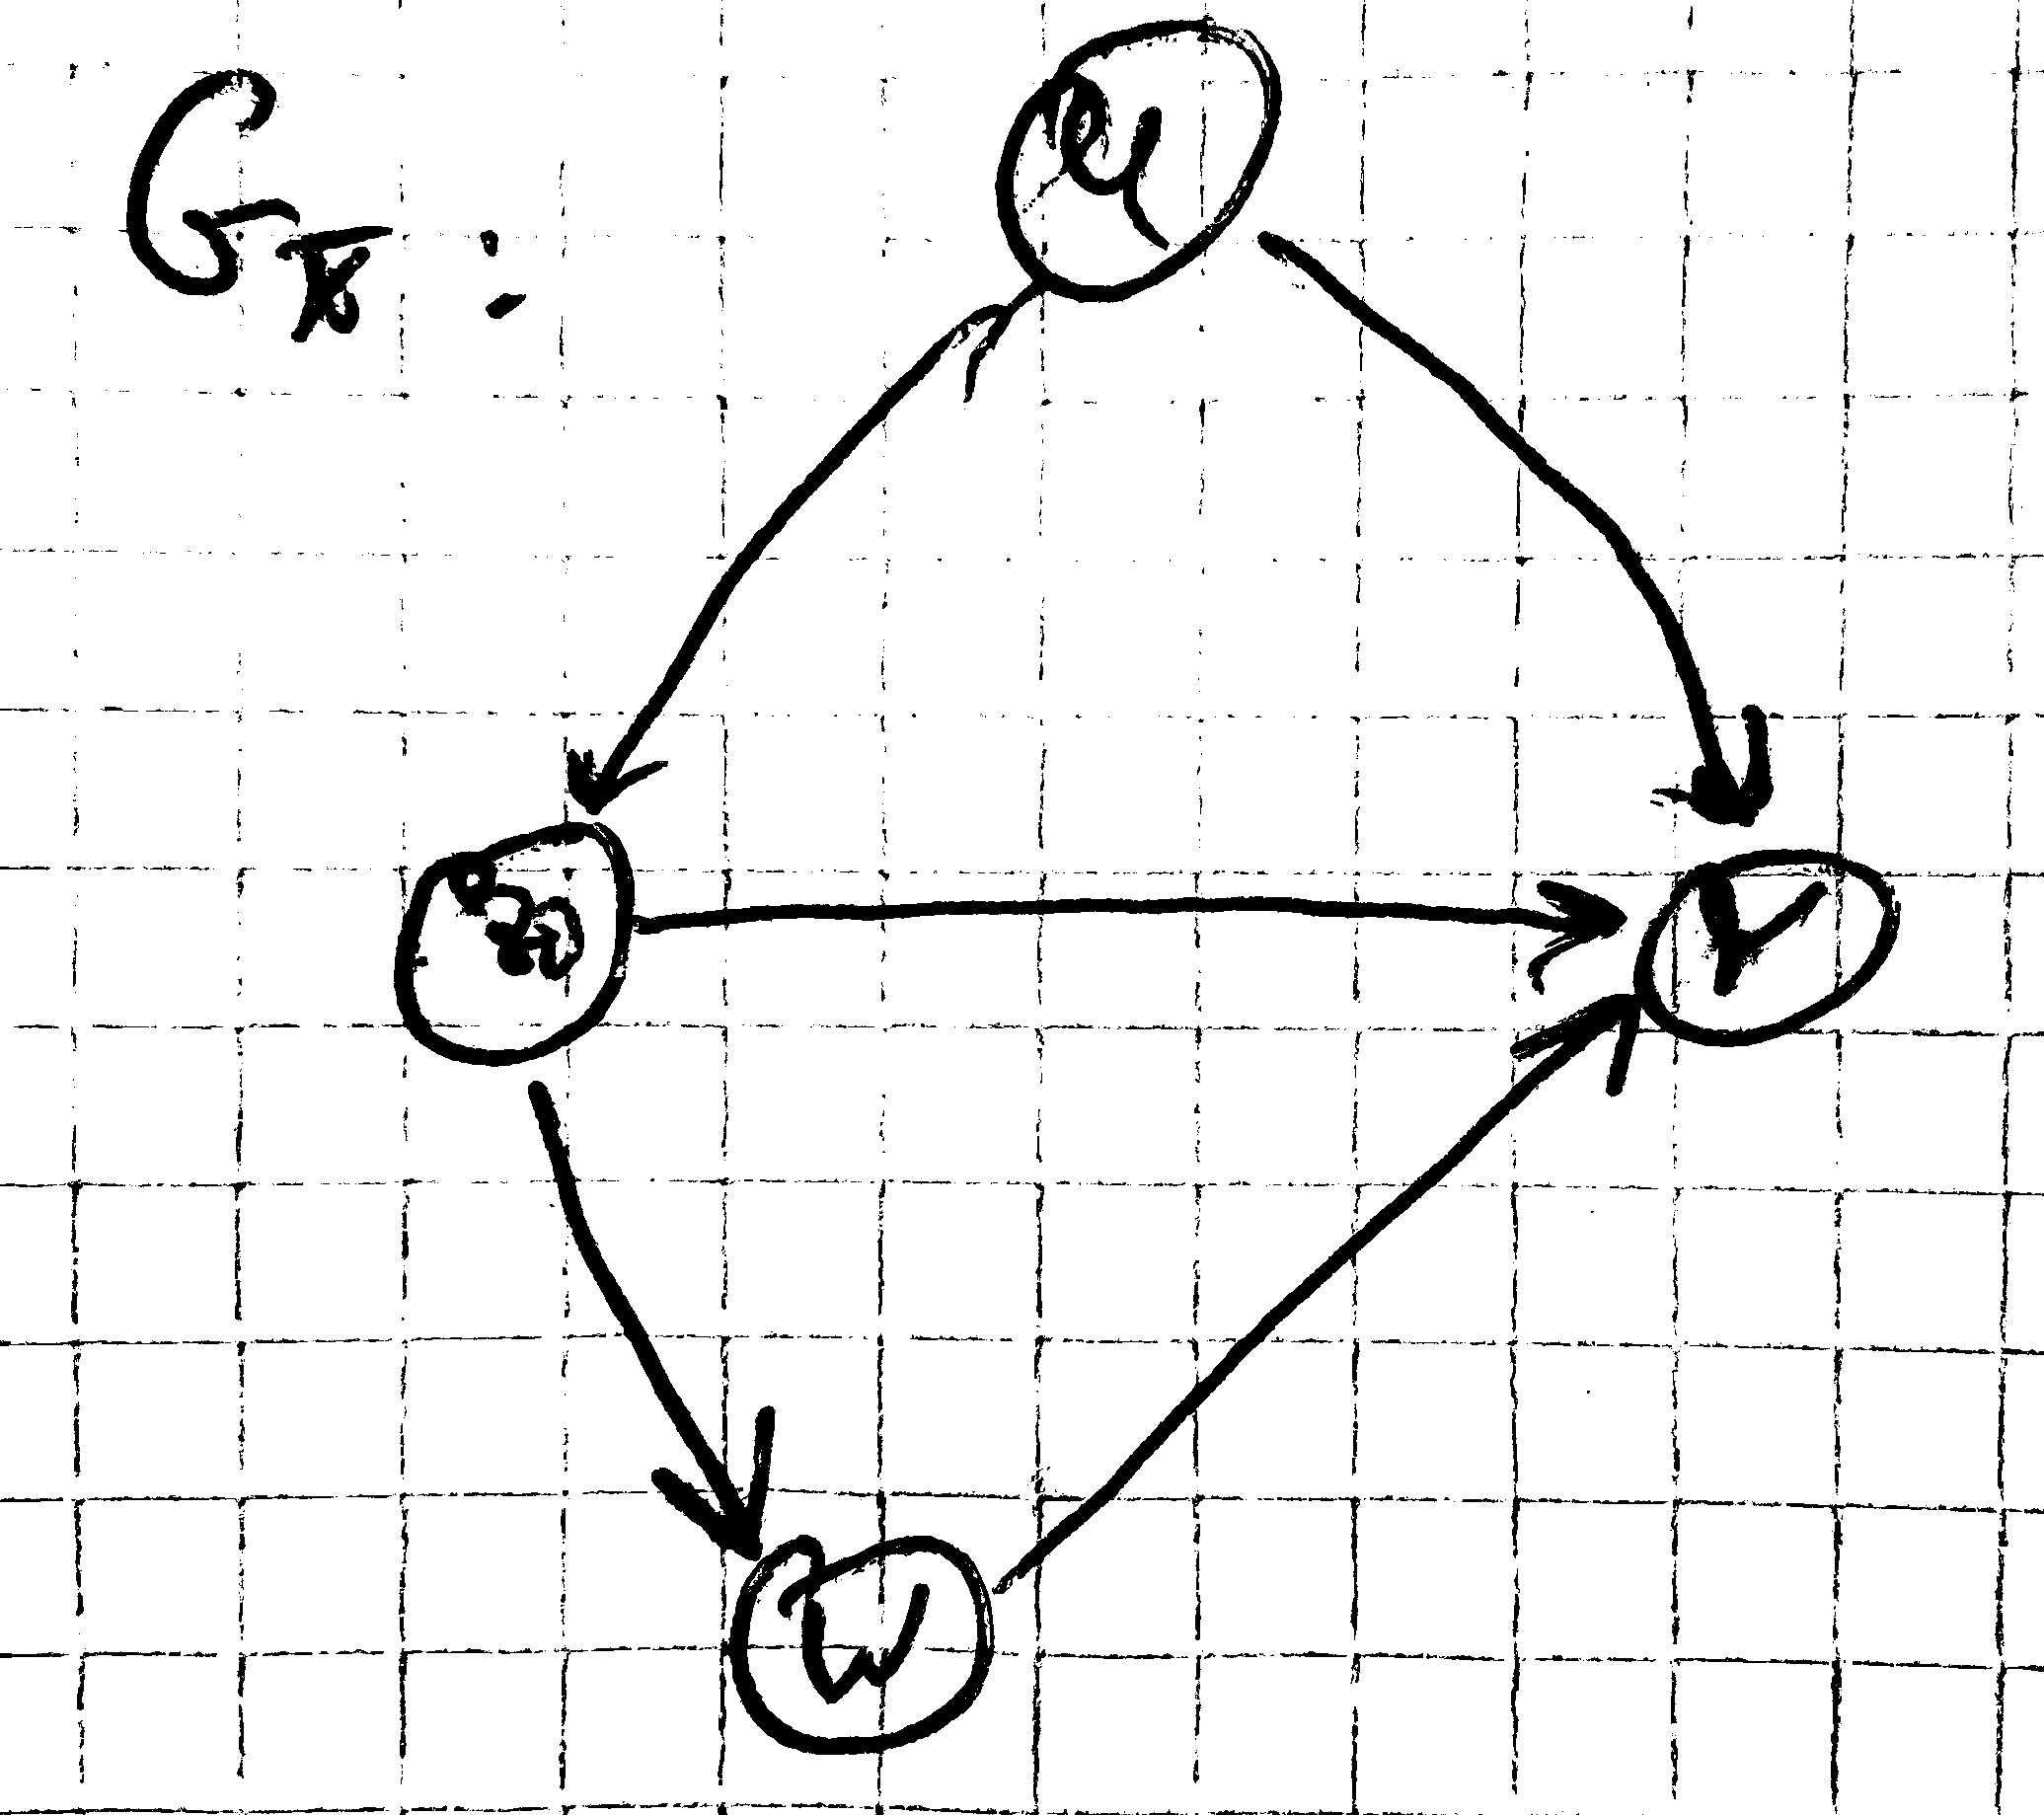
\includegraphics[scale=0.1]{imgs/img22.png}
	\end{center}
	\caption{$Z_i \notin Z(W)$}
	\label{fig:rule3_2}
\end{figure}

Corollary: If, by applying a finite number of rules 1-3 to the causal effect $P(y|\hat x_1,...,\hat x_m)$, we can obtain a formula without do-operators containing only observed quantities, then the causal effect is identifiable.

It has been shown that these rules are complete—that is, if the effect is identifiable, it can be shown by applying a set of such rules. However, the problem of determining whether such a set of rules exists remains complex and unsystematized.

\subsubsection*{Examples of Applying Inference Rules}

Consider the structure in Figure \ref{fig:rules_structure} and derive effects for it.

\begin{figure}[h]
	\begin{center}
		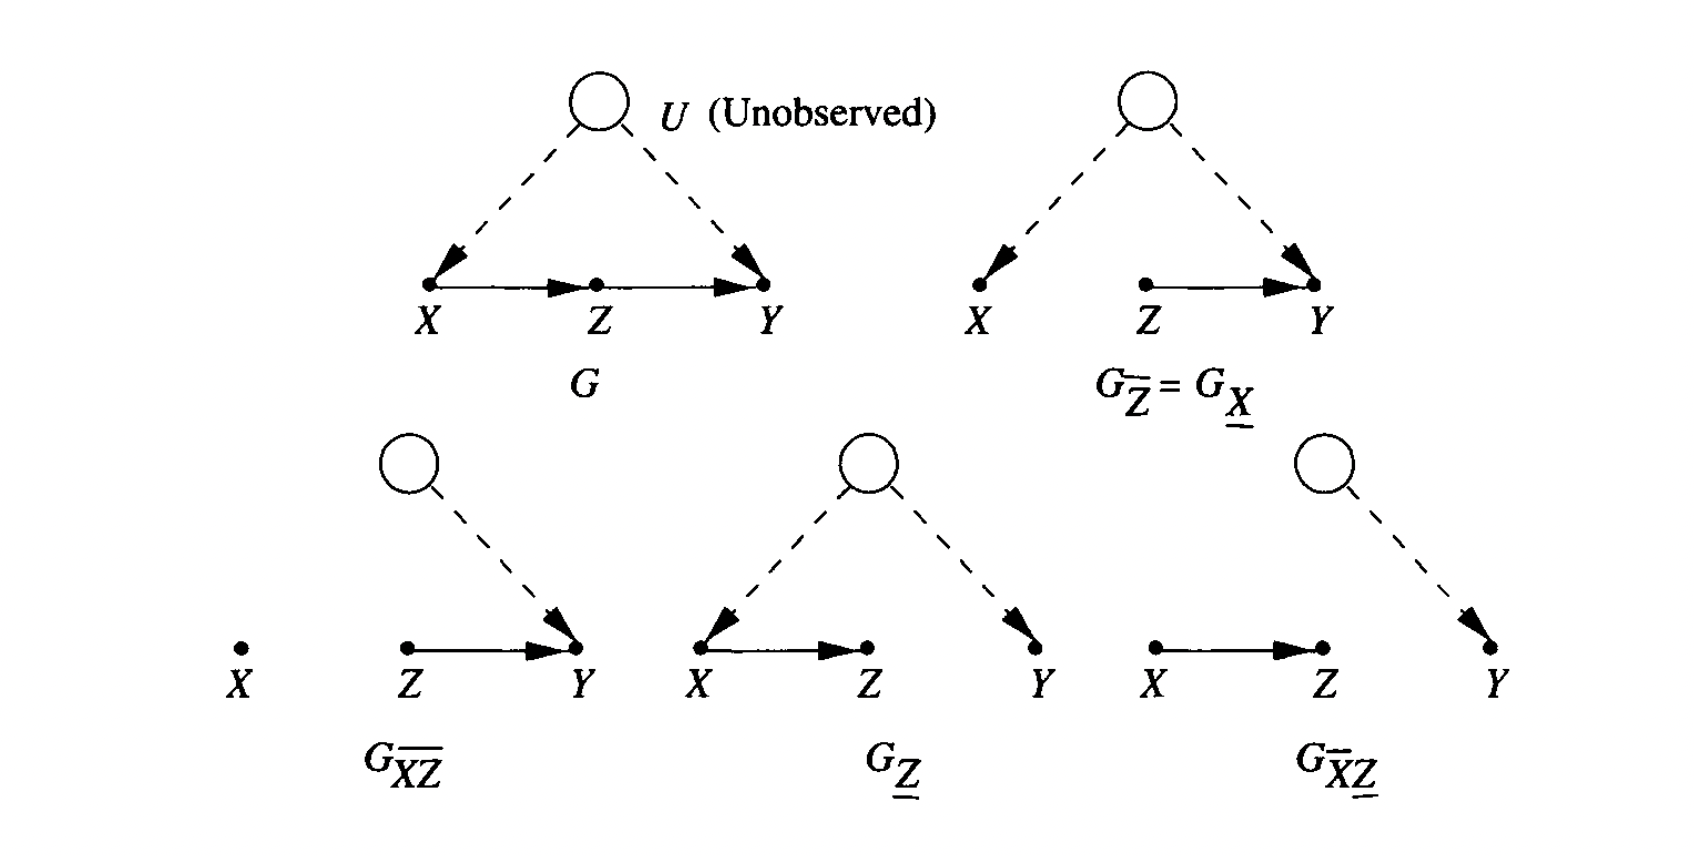
\includegraphics[scale=0.6]{imgs/img23.png}
	\end{center}
	\caption{$Z_i \notin Z(W)$}
	\label{fig:rules_structure}
\end{figure}

Problem 1. $P(z|\hat x)$ 

Note that $X \independent_{G_{\underline{X}}} Z$ (the only path is blocked by the unobserved $Y$), so by rule 2, $P(z|\hat x) = P(z| x)$.

Problem 2. $P(y|\hat z)$

$P(y|\hat z) = \sum\limits_{x}P(y|\hat z, x)P(x|\hat z)$

By rule 3, since $X \independent_{G_{\overline Z}}$, then $P(x|\hat z) = P(x)$.

By rule 2, since $Y \independent_{G_{\underline Z}} Z | X$, then $P(y|\hat z, x) = P(y| z, x)$.

Thus, we obtain the familiar backdoor adjustment formula: $P(y|\hat z) = \sum\limits_{x}P(y|z, x)P(x)$.

Problem 3. $P(y|\hat x)$

$P(y|\hat x) = \sum\limits_{z}P(y|\hat x, z)P(z|\hat x) = \sum\limits_{z}P(y|\hat x, z)P(z|x)$

The last equality is obtained from the solution to Problem 1, so it remains to derive $P(y|\hat x, z)$.

By rule 2, $P(y|\hat x, z) = P(y|\hat x, \hat z)$; by rule 3, $P(y|\hat x, \hat z) = P(y|\hat z)$. By Problem 2, $P(y|\hat z) = \sum\limits_{x}P(y|z, x)P(x)$.

Thus, we obtain $P(y|\hat x) = \sum\limits_{z}P(z|x)\sum\limits_{x'}P(y|z,x')P(x')$—which coincides with the front-door adjustment.

Problem 4. $P(y, z|\hat x)$

$P(y, z|\hat x) = P(y|z,\hat x)P(z|\hat x) = P(z|x)\sum\limits_{x'}P(y|z,x')P(x')$.

Problem 5. $P(y, x|\hat z)$

$P(y, x|\hat z) = P(y|x, \hat z) P(x|\hat z) = P(y|x,z)P(x)$

The last equality holds because $X$ blocks all backdoor paths from $Y$ to $Z$ (essentially, we applied rule 2), and to obtain the second term, we applied rule 3.

\subsection*{Graphical Tests for Identifiability}

\begin{figure}[h]
	\begin{center}
		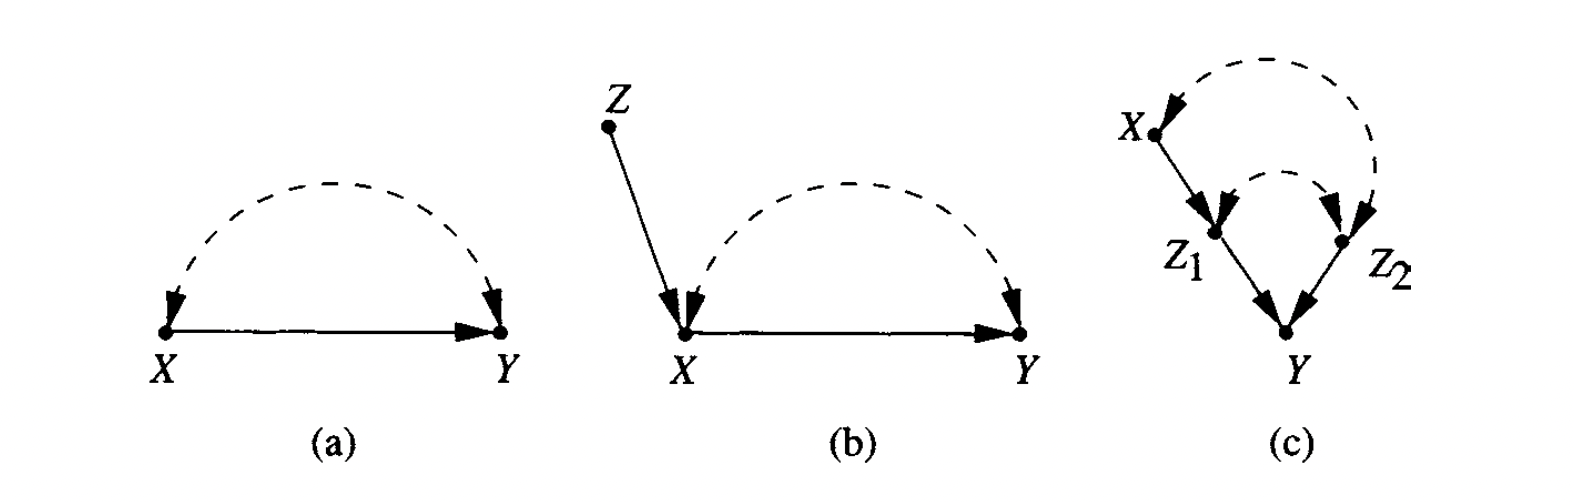
\includegraphics[scale=0.6]{imgs/img24.png}
	\end{center}
	\caption{Confounding arcs}
	\label{fig:confounding_arcs}
\end{figure}

In Figure \ref{fig:confounding_arcs}, we can see some examples of situations where the causal effect of $X$ on $Y$ is non-identifiable. In all these cases, the problem is due to the presence of a confounding arc. Such arcs are characterized by forming a backdoor path that contains only unobserved variables and has no $v$-structures: it is important to note that this is a backdoor path: indeed, if it were not so, we would have either a directed path $X \leadsto Y$ or a directed path $Y \leadsto X$. In general, we can recall how we characterized random associations: in their definition, it is important that neither of the two associated variables can be called the cause of the other.

\begin{figure}[h!]
	\begin{center}
		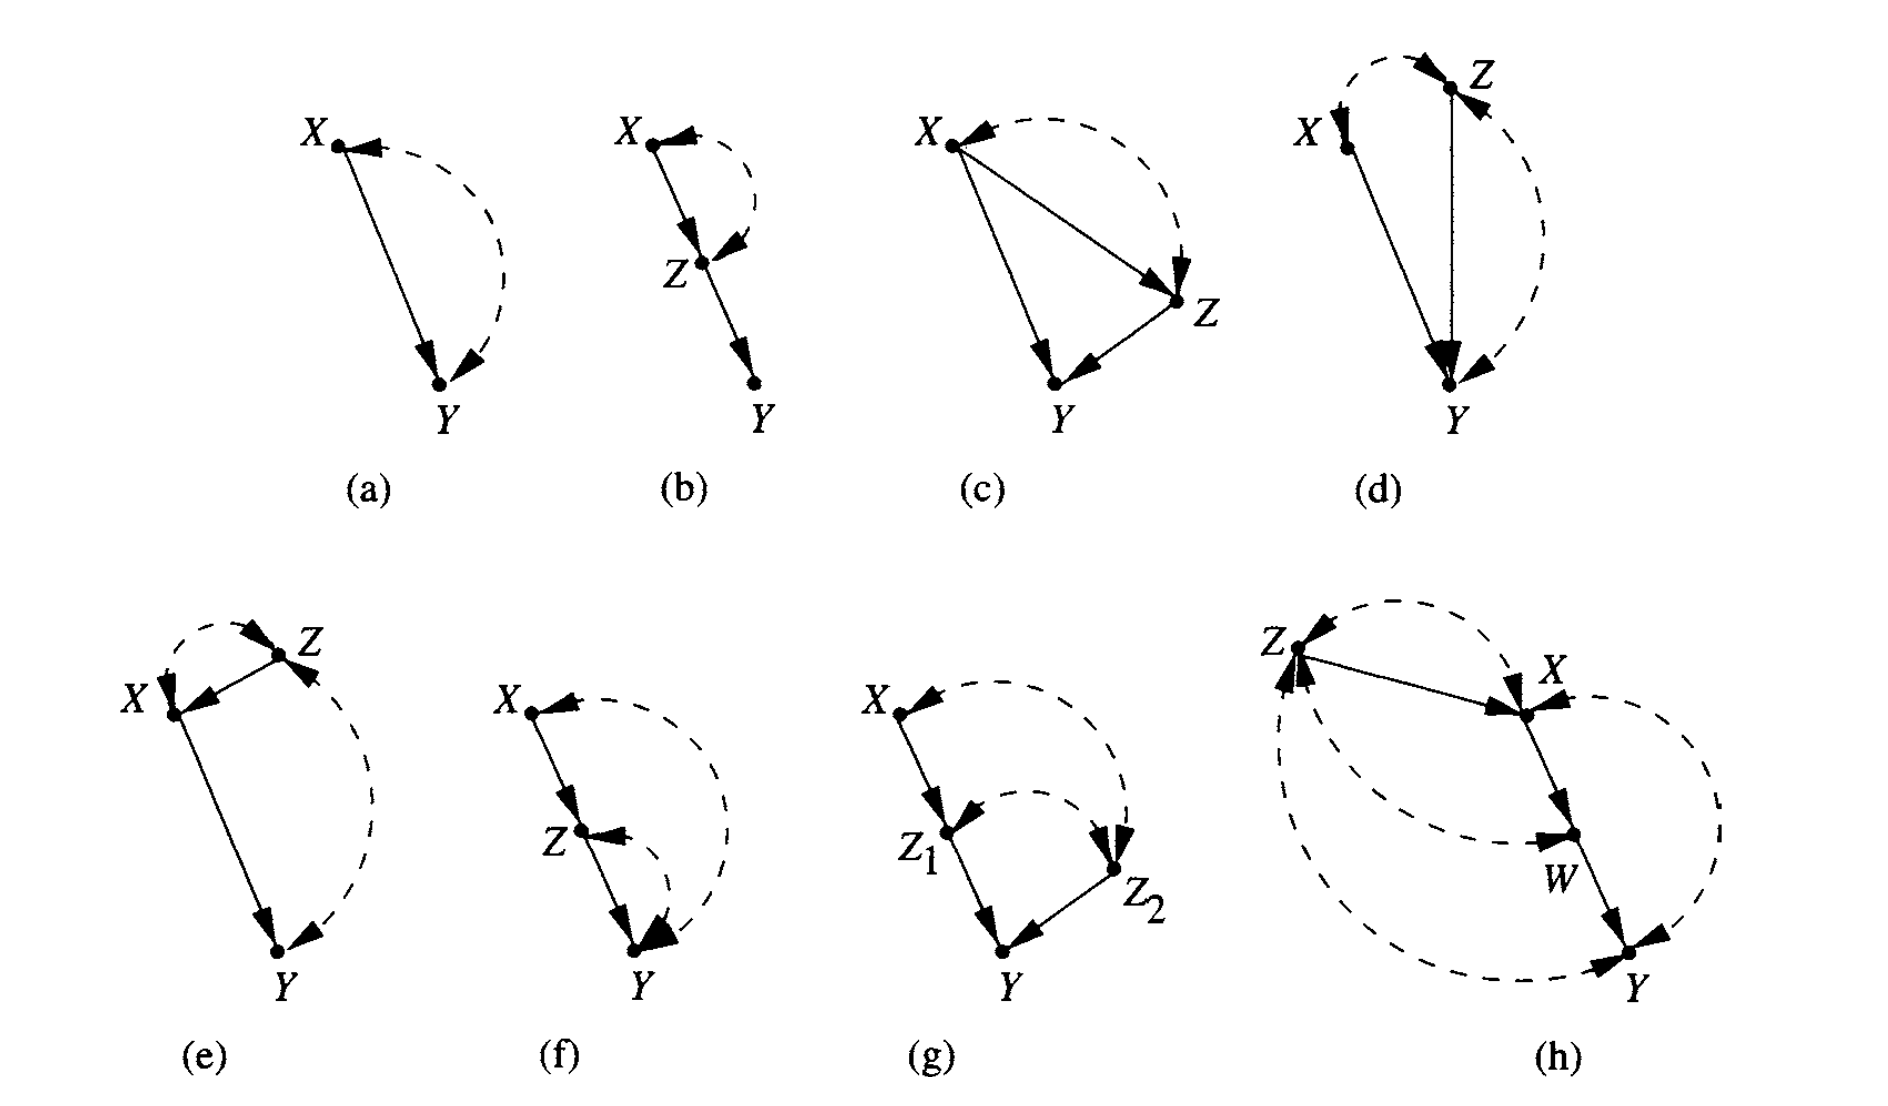
\includegraphics[scale=0.5]{imgs/img25.png}
	\end{center}
	\caption{Examples where confounding arcs lead to non-identifiability}
	\label{fig:confounding_arcs2}
\end{figure}

A characteristic feature is that adding variables and edges cannot lead to identifiability if such an arc exists, as in Figure \ref{fig:confounding_arcs} (b).

Another observation is that adding bidirectional arcs can worsen identifiability but not improve it: thus, if causal conclusions are unavailable in the original diagram, they are even more so in a diagram with additional arcs.

Interestingly, the ability to estimate the effect on individual parts does not always imply the ability to estimate the combined effect: for example, in \ref{fig:confounding_arcs} (c), we can estimate $P(z_1|\hat x) = P(z_1|x)$ (since $\emptyset$ satisfies the backdoor criterion relative to $(X, Z_1)$), and the book also claims the possibility of computing the effect $P(z_2|\hat x)$, but the impossibility of computing the effect $P(z_1, z_2 | \hat x)$. However, I have not yet managed to show the computability of the effect $P(z_2|\hat x)$ :(
UPDATE: seems I got it: note that $Z_2 \independent_{G_{\overline X}} X$, so by rule 3, $P(z_2 | \hat x) = P(z_2)$.

Another interesting observation: it turns out that the effect of a joint intervention may be computable, while the effects of partial interventions are not: referring again to \ref{fig:confounding_arcs} (c), we can see that $P(y|\hat x, \hat z_2)$ is identifiable, but $P(y|\hat x)$ is not.

When do we lack identifiability? It turns out that a sufficient condition for the impossibility of computing $P(y|\hat x)$ is the presence of an arc between $X \leftrightarrow Z$, where $Z \in de(X), Y \in de(Z)$. A necessary condition is the presence of an unblocked backdoor path from $Y$ to $X$ (unblocked by non-descendants of $X$).

For example, consider \ref{fig:confounding_arcs2} (b): write $P(y|\hat x) = \sum\limits_{z} P(y|\hat x, z) P(z | \hat x)$. $P(y|\hat x, z) = P(y|z)$ by rule 3, but $P(z | \hat x)$ is non-identifiable, as it corresponds to the situation in (a).

\section{Actions, Plans, and Direct Effects}

\subsection*{Introduction: Actions, Deeds, and Probabilities}

Actions can be interpreted from two perspectives: reactive and deliberative (passive and active). The reactive interpretation views an action as a consequence of the agent's assumptions, the current situation, and inputs from the external environment, e.g., "Adam ate the apple because Eve gave it to him." The deliberative interpretation views an action as a choice in decision-making, typically involving a comparison of consequences, e.g., "Adam was curious about what God would do if he ate the apple." We will distinguish these two viewpoints, calling the first a \textit{deed} and the second an \textit{action}.

A \textit{deed} is observed externally, while an \textit{action} is observed internally. Thus, a \textit{deed} can be predicted and can serve as evidence for certain motives and incentives of the actor (provided the actor is part of our model). \textit{Actions}, in turn, cannot be predicted nor provide any evidence, as by definition, they await a deliberate decision and turn into \textit{deeds} when executed.

Common-sense decision theory prescribes that rational agents choose the option $x$ that maximizes expected utility:

\begin{align}
	U(x) = \sum\limits_{y}P(y|do(x))u(y)
\end{align} 

where $u(y)$ is the utility of outcome $y$. In contrast, "evidential" decision theory prescribes maximizing the conditional expectation:

\begin{align}
	U_{ev}(x) = \sum\limits_{y}P(y|x)u(y)
\end{align} 
where $x$ is (incorrectly!) interpreted as an observed deed.

The paradoxes arising from this misconception are amusing and obvious: for example, one might conclude that patients should not visit doctors to reduce the likelihood of serious illness. Indeed, consider the following data:

\begin{align}
	\begin{tabular}{|c|c|c|c|}
		\hline
		sick & visited doctor? & probability & utility \\
		\hline yes & yes & 0.35 & -80 \\
		\hline no & yes & 0.15 & 90  \\
		\hline yes & no & 0.15 & -100 \\
		\hline    no & no & 0.35 & 100 \\ \hline
	\end{tabular}
\end{align}

Then $U_{ev}(x=\text{visit doctor}) = -29$, while $U_{ev}(x=\text{do not visit}) = +40$.

Similarly, workers should not rush to work to avoid being late, and students should not study for exams if they want to pass. Generalizing, we arrive at the paradox stating that measures to improve the situation should be avoided, lest these measures increase the probability that they were indeed necessary.

The strangeness of this logic stems from attempting to treat actions as deeds determined by prior associations, instead of perceiving them as objects of free choice, as dictated by the semantics of the $do$-operator. Evidential decision theory claims that statistical evidence cannot be ignored (in our case, evidence for whether certain deeds were necessary or not), but the correct theory reminds us that actions, by definition, make such evidence irrelevant to the current decision, as actions \textit{change} the probabilities that deeds typically obey.

A nice poem, quoting as-is:

\begin{center}
	\textit{Whatever evidence an act might provide\\
		On what could have caused the act, \\
		Should never be used to help one decide \\
		On whether to choose that same act.}
\end{center}

\subsection*{Conditional Actions and Stochastic Policies}

Previously, we considered only the simplest interventions, consisting of setting some set of variables to a fixed value. In the general case, an intervention may consist of a variable behaving according to some specific law dependent on the values of other variables: $x = g(z)$, or via a stochastic relation, where $X$ is set to $x$ with probability $P^*(x|z)$. Below, we will show that identifying such interventions is equivalent to identifying $P(y|\hat x, z)$.

\begin{align}
	\begin{split}
		P(y|do(X=g(z))) &= \sum\limits_{z}P(y|do(X=g(z)),z)P(z|do(X=g(z)))\\
		& = \sum\limits_{z}P(y|\hat x,z)_{x=g(z)}P(z) \\
		&= \mathbb{E}_zP(y|\hat x, z)_{x=g(z)}
	\end{split}
\end{align}

$P(z|do(X=g(z))) = P(z)$, since $Z$ is not a descendant of $X$ (if it were, we would end up with a cyclic graph after the intervention, which is probably undesirable and unlikely to make physical sense in practice), so no intervention on $X$ can influence $Z$ (in the post-intervention world, $X$ is independent of all its non-descendants, which can be derived, e.g., from rule 3 of do-calculus). Thus, the effect of an intervention with policy $do(X=g(z))$ can be computed directly from the expression $P(y|\hat x,z)$ by substituting $x=g(z)$ and taking the expectation of this quantity.

The identifiability criterion for a conditional policy is stricter than for an unconditional one: indeed, if $P(y|do(X=g(z)))$ is identifiable, then setting $g(z) = x$ (a constant), we find that the atomic intervention is also identifiable. The converse, however, is not always true: conditioning on $Z$ may introduce additional dependencies that can hinder the transformation of $P(y|\hat x, z)$ into an expression without do-operators.

A stochastic policy, where $X$ behaves according to $P^*(x|z)$, can be considered similarly: such a policy means we perform the intervention $do(X=x)$ with probability $P^*(x|z)$. Thus, we can write:

\begin{align}
	\begin{split}
		P(y|do(X \sim P^*(x|z))) &= \sum\limits_{x}\sum\limits_{z}P(y|\hat x,z)P^*(x|z)P(z)
	\end{split}
\end{align}

We arrive at the conclusion that a necessary and sufficient condition for the identifiability of a stochastic policy is also the identifiability of $P(y|\hat x, z)$.

\subsection*{When Is the Effect of an Action Identifiable?}

The following two theorems describe necessary and sufficient conditions for the identifiability of the effect of one variable on another.

\begin{theorem}
	\label{th:sufficient_identify}
	Let $X$ and $Y$ be two variables in a semi-Markovian model characterized by graph $G$ (DAG, but unmeasured variables may have more than one descendant). A sufficient condition for the identifiability of $P(y|\hat x)$ is that $G$ satisfies at least one of the following four conditions:
	
	1. There is no backdoor path from $X$ to $Y$, i.e., $X \independent_{G_{\underline{X}}} Y$.
	
	2. There is no directed path from $X$ to $Y$.
	
	3. There exists a set of vertices $B$ that blocks all backdoor paths from $X$ to $Y$ such that $P(b|\hat x)$ is identifiable (a special case is when all vertices in $B$ are non-descendants of $X$, then $P(b|\hat x) = P(b)$).
	
	4. There exist sets $Z_1 \subset de(X), Z_2: Z_2 \cap de(X) = \emptyset$:
	
	(i) $Z_1$ blocks every directed path from $X$ to $Y$ in $G_{\overline{Z_1}}$: i.e., $Y \independent_{G_{\overline{Z_1}\overline{X}}} X | Z_1$.
	
	(ii) $Z_2$ blocks all backdoor paths between $Z_1$ and $Y$ in $G_{\overline{X}}$: $Y \independent_{G_{\underline{Z_1}\overline{X}}} Z_1 | Z_2$.
	
	(iii) $Z_2$ blocks all backdoor paths between $X$ and $Z_1$: $X \independent_{G_{\underline{X}}} Z_1 | Z_2$.
	
	(iv) $Z_2$ does not activate any backdoor path from $X$ to $Y$: $X \independent_{G_{\overline{X(Z_2)} \overline{Z_1}}} Y | Z_1, Z_2$.
\end{theorem}

Proof:

1. This condition means $Y \independent_{G_{\underline{X}}} X$, so we can directly apply rule 2 of do-calculus, i.e., $P(y|\hat x) = P(y|x)$.

2. This condition means $Y$ is not a descendant of $X$ in the graph, so $P(y|\hat x) = P(y)$—this follows from rule 3 of do-calculus: $Y \independent_{G_{\overline{X}}} X$.

3. In this case, write $P(y|\hat x) = \sum\limits_{b} P(y|\hat x, b)P(b|\hat x)$.

Next, using the backdoor criterion (or rule 2 of do-calculus), $P(y|\hat x, b) = P(y|x, b)$, and since $P(b|\hat x)$ is also identifiable by condition, then $P(y|\hat x) = \sum\limits_{b} P(y|x, b)P(b|\hat x)$ is identifiable.

4. Here, we need to work harder:

$P(y|\hat x) = \sum\limits_{z_1,z_2}P(y|\hat x, z_1, z_2)P(z_1,z_2|\hat x)$.

$P(y|\hat x, z_1, z_2) = P(y| \hat x, \hat z_1, z_2)$ by rule 2, since $Z_2$ blocks all backdoor paths between $Z_1$ and $Y$.

Next, $P(y| \hat x, \hat z_1, z_2) = P(y|\hat z_1, z_2)$ by rule 3, since $Y \independent_{G_{\overline{Z_1} \overline{X(Z_2)}}} X | Z_2, Z_1$.

To eliminate the hat here, we can write $P(y|\hat z_1, z_2) = \sum\limits_{x'} P(y|\hat z_1, z_2, x')P(x'|\hat z_1, z_2)$. Note that $P(y|\hat z_1, z_2, x') = P(y|z_1, z_2, x')$, since by (ii) and (iii), the only possible backdoor path between $Z_1$ and $Y$, not blocked by $Z_2$, must have an edge entering $X$ and an edge leaving $X$: indeed, if there were no edge entering $X$, then by (ii), such a path would be blocked in $G_{\underline{Z_1}}$ by $Z_2$, meaning it would also be blocked in the original graph (since it is a backdoor path relative to $Z_1$). If there is no edge leaving $X$, then $X$ forms a $v$-structure in this path, meaning $Z_2$ must block part of this path between $Z_1$ and $X$ by (iii), as this part is a backdoor path from $X$ to $Z_1$. But such a path (of the form $Z_1 \leadsto ... \rightarrow X \rightarrow ... \leadsto Y$) will be blocked if we condition on $X$, which we indeed do.

Using the above reasoning, we conclude that by rule 2, $P(y|\hat z_1, z_2, x) = P(y|z_1, z_2, x)$.

Next, note that $P(x'|\hat z_1, z_2) = P(x'|z_2)$, since $Z_1$ are descendants of $X$, so an action on them does not affect $X$.

\begin{align}
	P(y|\hat x, z_1, z_2) = \sum\limits_{x'} P(y|z_1, z_2, x')P(x'|z_2)
\end{align}
	
	
Now consider $P(z_1, z_2 | \hat x) = P(z_1 | \hat x, z_2) P(z_2 | \hat x)$. Note that since $Z_2$ contains no descendants of $X$, then $P(z_2|\hat x) = P(z_2)$ (this follows from rule 3 of do-calculus). $P(z_1 | \hat x, z_2) = P(z_1 | x, z_2)$, because $Z_2$ blocks all backdoor paths from $X$ to $Z_1$ according to (ii).

Thus, we arrive at the complete expression:

\begin{align}
	P(y|\hat x) = \sum\limits_{z_1,z_2}P(z_1|x, z_2)P(z_2)\sum\limits_{x'} P(y|z_1, z_2, x')P(x'|z_2)
\end{align}

$\blacksquare$

\begin{theorem}
	\textbf{Necessary condition for identifiability} At least one of the conditions of Theorem \ref{th:sufficient_identify} is necessary for the identifiability of $P(y|\hat x)$. 
\end{theorem}

We will prove by contradiction: assume there exists a graph G and $P(y|\hat x)$ such that none of the four conditions holds, but $P(y|\hat x)$ is identifiable, and show that this leads to a contradiction.

Since the expression is identifiable, there exists some finite sequence of applications of rules 1-3 of do-calculus that reduces the expression to a hat-free form. To remove the hat from $x$, we have only two rules out of three:\\
\textbf{Case 1}: applying rule 2: $P(y|\hat x, \hat z, w) \to P(y|x, \hat z, w)$ if $Y \independent_{G_{\overline Z \underline{X}}} X | Z, W$ \\
\textbf{Case 2}: applying rule 3: $P(y|\hat x, \hat z, w) \to P(y|\hat z, w)$ if $Y \independent_{G_{\overline{Z}\overline{X(W)}}} X | Z, W$ (Case 2)

Let's consider each of these two cases in turn.

\textbf{Case 1}
There exist some subsets $X,W$: $Y \independent_{G_{\overline Z \underline{X}}} X | Z, W$. Without loss of generality, assume $Z, W$ are minimal; otherwise, we can remove redundant vertices and prove for such sets.

If it were $Y \independent_{G_{\underline{X}}} X | Z, W$, then the set $Z \cup W$ would block all backdoor paths from $X$ to $Y$, but then condition 3 \ref{th:sufficient_identify} would hold. However, it's unclear why we assumed that $P(z,w | \hat x)$ is identifiable? Honestly, I don't understand yet; it seems like an inaccuracy in the proof.

The proof of this theorem can be found in Galles, Pearl (1995); I'm too lazy to look for it now.
$\blacksquare$

\subsubsection*{Notes on Efficiency}

Conditions 3 and 4 of Theorem \ref{th:sufficient_identify} require exhaustive enumeration of possible sets $B$ and $Z_1, Z_2$. However, the following theorems allow significantly reducing the search space.

\begin{theorem}
	If $P(b_i|\hat x)$ is identifiable for some minimal set $B_i$, then $P(b_j|\hat x)$ is identifiable for any other minimal set $B_j$.
\end{theorem}

This theorem allows checking identifiability for any minimal set blocking all backdoor paths and making a verdict based on the result - whether condition 3 of Theorem \ref{th:sufficient_identify} holds or not.

To prove this theorem, we use the lemma:

\begin{lemma}
	If the expression $P(y|\hat x)$ is identifiable and the set of vertices $Z$ lies on a directed path from $X$ to $Y$, then $P(z|\hat x)$ is also identifiable.
\end{lemma}

\begin{theorem}
	Let $Y_1$, $Y_2$ be two subsets of vertices such that one of the following holds:
	
	(i) $Y_1 \cap de(X) = \emptyset$
	
	(ii) $Y_1 \cup Y_2 \subset de(X)$ and $Y_1 \cap de(Y_2) = \emptyset$
	
	Then $P(y_1, y_2 | \hat x)$ is identifiable $\iff P(y_1|\hat x)$ and $P(y_2|\hat x, y_1)$ are identifiable.
\end{theorem}

Well, the left arrow is obvious: $P(y_1, y_2 | \hat x) = P(y_1|\hat x)P(y_2|\hat x, y_1)$, so the derivability of the right side indeed implies the derivability of the left side.

The right arrow is less obvious.

\begin{theorem}
	If there exists $Z_1$ satisfying condition 4 of Theorem \ref{th:sufficient_identify}, then the set consisting of children of $X$ intersected with ancestors of $Y$ will also satisfy the conditions imposed on $Z_1$. 
\end{theorem}

This theorem makes the search for set $Z_1$ trivial.

\subsubsection*{Algorithm for deriving $P(y|\hat x)$}

\textbf{Algorithm ClosedForm}

\textbf{Input:} Query $P(y|\hat x)$

\textbf{Output:} Either an expression for $P(y|\hat x)$ in closed form containing only observed variables, or FAIL if the expression is not identifiable.

1. If $X \independent_{G_{\overline X}} Y$ then return $P(y)$

2. Else if $X \independent_{G_{\underline{X}}}$ then return $P(y|x)$

3. Else, let $B = BlockingSet(X, Y)$, $Pb = ClosedForm(P(b|\hat x))$. If $Pb \neq FAIL$, return $\sum\limits_{b}P(y|x,b)Pb$

4. Else, let $Z_1 = Children(X) \cap (Y \cup Ancestors(Y))$, $Z_3 = BlockingSet(X, Z_1)$, $X_4 = BlockingSet(Z_1, Y)$, $Z_2 = Z_3 \cup Z_4$. If $Y \notin Z_1$ and $X \notin Z_2$, return $\sum\limits_{z_1, z_2}P(z_1|x,z_2)P(z_2)\sum\limits_{x'}P(y|z_1, z_2, x')P(x'|z_2)$

5. Else, return FAIL.

There's a trick with this algorithm: during recursive calls, it may turn out that $P(b|\hat x)$ is called with $|B| > 1$, but the original theorem about the necessity and sufficiency of one of the four conditions was proven only for single variables $X, Y$.

\subsection*{Identification of Dynamic Plans}

\subsubsection*{Motivation}

Consider an example with a causal graph as in \ref{fig:dynamic_plan}. $X_1, X_2$ denote treatments prescribed by doctors, $Z$ - observations based on which the second doctor makes a decision about the type of $X_2$, and $Y$ - whether the patient survived. Unobserved variables: $U_1$ - part of the patient's history, $U_2$ - the patient's propensity to recover.

\begin{figure}[h]
	\begin{center}
		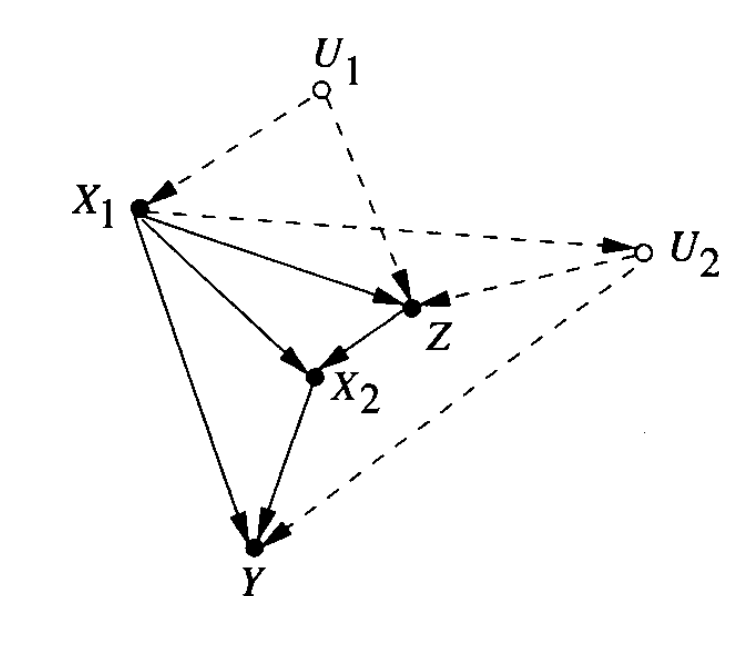
\includegraphics[scale=0.6]{imgs/img26.png}
	\end{center}
	\caption{Task of estimating the effect of the plan $(do(x_1), do(x_2))$ on $Y$}
	\label{fig:dynamic_plan}
\end{figure}

A real-world example of such a graph could be a speed-related comorbidity PCP - pneumocystis pneumonia - corresponding to $Z$ in the graph. It is effectively treatable, so it has no direct effect on survival $Y$, but it is an indicator that the patient's immune state $U_2$ is not in the best condition, which in turn can lead to death. $X_1, X_2$ in this case denote the intake of Bactrim - a drug that fights PCP and can also prevent death from other causes. For prescribing Bactrim, doctors rely in part on the patient's earlier PCP history, but suppose it was not recorded for our analysis.

We are faced with the following task: there is a large dataset $(X_1, Z, X_2, Y)$. Then, a patient comes to us, and we need to estimate the effect of the unconditional plan $(do(x_1), do(x_2))$ on their survival. In general, what we need to do is develop an action plan based on the observed already executed actions (acts) of other actors whose strategies are unknown to us.

In this case, we again face the identification task, which, as before, is non-trivial due to confounding links. In the case of plan identification, however, there is an additional complexity - some confounders are affected by controlled variables (for example, $Z$ - is affected by $X_1$).

In this case, we can identify $P(y | \hat x_1, \hat x_2)$:

\begin{align}
	\begin{split}
		P(y | \hat x_1, \hat x_2) &= P(y|x_1, \hat x_2) \\
		&= \sum\limits_{z} P(y|x_1,z, \hat x_2)P(z|x_1,\hat x_2)\\
		&= \sum\limits_{z} P(y|x_1,z, x_2)P(z|x_1)\\
	\end{split}
\end{align}

The first transition follows from rule 2 (since $Y \independent_{G_{\overline X_2 \underline{X_1}}} X_1 | X_2$). The second transition is simply marginalization of the joint distribution on $Y,Z | X_1, X_2$. The third - we use that $Z$ is not a descendant of $X_2$, so the intervention on $X_2$ does not affect it (by rule 3), and $X_1, Z$ blocks all backdoor paths between $X_2$ and $Y$, so the first factor transforms by rule 2.

\subsubsection*{Notation and Assumptions in Plan Identification}

We start by assuming the causal diagram is known, which provides a qualitative understanding of the data-generating process.

The control task is defined by a DAG G with vertices consisting of four disjoint sets $V = \{X,Z,U,Y\}$ where:

$X$ - set of controlled variables

$Z$ - set of observed covariate variables

$U$ - set of unobserved (latent) variables

$Y$ - outcome variable

Let's number the controlled variables $X_1,X_2,...,X_n$ such that $X_k$ has no directed paths to $X_1,...,X_{k-1}$, and also $Y$ is a descendant of $X_n$. A plan is an ordered sequence $(\hat x_1, ..., \hat x_n)$. A conditional plan is an ordered sequence $\hat g_1(z_1), ..., \hat g_n(z_n)$ where $g_k$ is a function from $Z_k$ to $X_k$, $\hat g_k(z_k)$ means setting $X_k$ to $g(z_k)$, and $Z_k$ contains no descendants of $X_k$ relative to G.

The task is to compute the effect of the unconditional plan on variable $Y$ $P(y|\hat x_1, ...\hat x_n)$.

\subsubsection*{Plan Identification: Sequential Backdoor Criterion}

\begin{theorem}
	$P(y|\hat x_1, ...\hat x_n)$ is identifiable if $\forall 1 \le k \le n \ \exists Z_k \subset Z:$ 
	
	1. $ \forall j > k \ Z_k \cap de(X_j) = \emptyset$
	
	2. $Y \independent_{G_{\underline{X}_k}\overline{X}_{k+1},..,\overline{X}_n} X_k | X_1, ..., X_{k-1}, Z_1, ..., Z_k$
	
	In this case, the plan effect is expressed by the formula:
	
	\begin{align}
		\sum\limits_{z_1,..,z_n}P(y|z_1,...,z_n,x_1,...,x_n)\prod\limits_{k=1}^nP(z_k|z_1,..z_{k-1}, x_1,....,x_{k-1})
	\end{align}
\end{theorem}

Proof: since $Z_k$ contains no descendants of $X_j$ $\forall \ j > k$, then by rule 3 of do-calculus:

\begin{align}
	P(z_k|z_1,..,z_{k-1},x_1,..,x_{k-1}, \hat x_k, ...,\hat x_n) = P(z_k|z_1,..,z_{k-1},x_1,..,x_{k-1}) 
\end{align}

Condition 2 of the theorem allows us to apply rule 2:

\begin{align}
	P(y|z_1,..,z_{k},x_1,..,x_{k-1}, \hat x_k, ...,\hat x_n) = P(z_k|z_1,..,z_{k-1},x_1,..,x_k,\hat x_{k+1},...,\hat x_n) 
\end{align}

removing the hat from $x_k$.

Thus, we obtain:

\begin{align}
	\begin{split}
		P(y|\hat x_1,...,\hat x_n) &= \sum\limits_{z_1}P(y|z_1,\hat x_1,...,\hat x_n)P(z_1|\hat x_1,...,\hat x_n) \\
		&=  \sum\limits_{z_1}P(y|z_1, x_1,...,\hat x_n)P(z_1) \\
		&= \sum\limits_{z_1,z_2}P(y|z_1, z_2, x_1, \hat x_2,...,\hat x_n)P(z_1)P(z_2|x_1,\hat x_2,...,\hat x_n) \\
		&=\sum\limits_{z_1,z_2}P(y|z_1, z_2, x_1, x_2,...,\hat x_n)P(z_1)P(z_2|x_1,z_1)\\
		&= \ldots \\
		&= \sum\limits_{z_1,...,z_n}P(y|z_1, z_2, ..., z_n, x_1, x_2,...,x_n)\prod\limits_{k=1}^nP(z_k|x_1,...,x_{k-1},z_1,...,z_{k-1})
	\end{split}
\end{align}

$\blacksquare$

The control task is called \textit{G-identifiable} if $P(y|\hat x_1,...,\hat x_n)$ is identifiable using the criterion from the previous theorem. The sequence of corresponding covariates $Z$ is called \textit{admissible}.

It is worth noting that G-identifiability $\implies$ identifiability, but not vice versa: indeed, at the k-th step, general identifiability may hold even when conditioning on $Z_k$ containing descendants of $X_k$ - variables that may be affected by the action $do(X_k=x_k)$, but this is prohibited in $G$-identifiability.

\subsubsection*{Plan Identification: Procedure}

So far, we have only declaratively described how to identify a plan. However, it is not yet clear how to choose the sets $Z_k$, and whether any choice will work. In Figure \ref{fig:bad_admissible_set}, we can see an example where choosing an unfortunate $Z_1$ makes further choices of sets impossible.

\begin{figure}[h]
	\begin{center}
		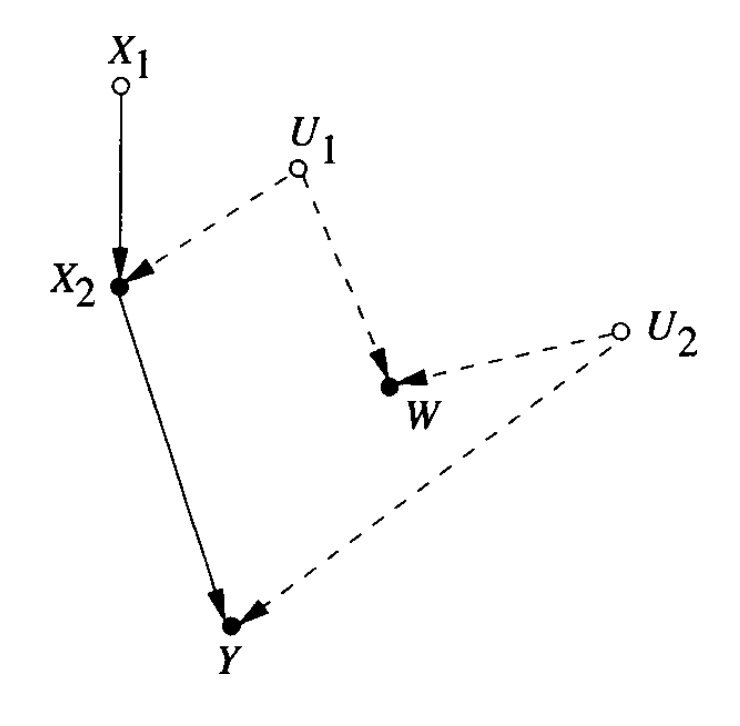
\includegraphics[scale=0.6]{imgs/img27.png}
	\end{center}
	\caption{Choosing $Z_1=\{W\}$ makes it impossible to choose any admissible $Z_2$}
	\label{fig:bad_admissible_set}
\end{figure}

\begin{theorem}
	If there exists an admissible sequence $Z_1^*,...,Z_n^*$, then for any \textbf{minimal} admissible subsequence $Z_1,...,Z_{k-1}$ there exists an admissible set $Z_k$.
\end{theorem}

Proof in Pearl and Robins (1995) $\blacksquare$

Corollary: the control task is G-identifiable if and only if the following algorithm returns success:

1. $k := 1$

2. Choose any $Z_k \subset Z \backslash (de(X_k) \cup ... \cup de(X_n))$ 

3. If $Z_k$ is not found, return FAIL, else $k := k + 1$

4. If $k = n + 1$, return OK

The following theorem allows efficient selection of $Z_k$:

\begin{theorem}
	\label{th:plan_identification}
	The plan effect $P(y|\hat x_1,...,x_n)$ is G-identifiable $\equiv$ $\forall k \in [1,...,n]$ $Y \independent_{G_{\underline{X}_k,\overline{X}_{k+1},...,\overline{X}_n}}X_k | X_1,..,X_{k-1},W_1,...,W_k$ where $W_k$ are covariates that contain no descendants of $X_k,...,X_n$ and have as descendants either $Y$ or $X_k$ in the graph $G_{\underline{X}_k,\overline{X}_{k+1},...,\overline{X}_n}$. 
	
	In this case, the plan effect is expressed as:
	
	\begin{align}
		\sum\limits_{w_1,...,w_n}P(y|w_1, w_2,...,w_n x_1, x_2,...,x_n)\prod\limits_{k=1}^nP(w_k|x_1,...,x_{k-1},w_1,...,w_{k-1})
	\end{align}
\end{theorem}

Proof again in Pearl and Robins (1995) $\blacksquare$

It is worth noting that despite the fact that the deterministic efficient algorithm in \ref{th:plan_identification} allows determining G-identifiability, it still depends on the chosen order $X_1,...,X_n$. It is not excluded that for one order admissible by graph G, an admissible sequence of covariates exists, while for another - it does not.

This means that to verify that the plan is not G-identifiable, it is necessary to check all orders of controlling variables admissible by the graph.

\subsection*{Direct and Indirect Effects}

The causal effect we have been studying so far $P(y|\hat x)$ is the total effect of the variable/set of variables $X$ on $Y$. In many cases, however, we are interested not in it, but in the direct effect - the effect that is not mediated through other variables - or, more precisely - the effect of changing $X$ when all other variables are fixed.

An example where the direct effect may be of interest is when we want to estimate the effect of birth control pills on blood clots: on the one hand, there is a hypothesis that the pills increase clot formation. On the other hand, there is an indirect negative effect on clot formation, as pregnancy increases their probability.

Another example is analyzing the presence of discrimination based on gender: in this case, the question of the direct influence of gender on the hiring result is of interest, while the influence of gender or race on qualifications, as well as the influence of qualifications, is not the subject of investigation.

\subsubsection*{Direct Effects: Definition and Identification}

\define{Direct effect} is defined as $P(y|\hat x, \hat s_{XY})$, where $s_{XY}$ is the set of all endogenous (observed) variables of the system except $X,Y$.

Note that controlling all possible variables is generally not necessary - it is sufficient to control all immediate parents of $Y$: indeed, in this case, no directed path to $Y$, except the edge $X \rightarrow Y$, will be active.

\begin{corollary}
	The immediate effect of $X$ on $Y$ is given by $P(y|\hat x, \hat{pa}_{Y \backslash X})$, where $\hat{pa}_{Y \backslash X})$ is any realization of all parents of $Y$, except $X$.
\end{corollary}

Clearly, if $X$ is not a parent of $Y$, then $P(y|\hat x, \hat{pa}_{Y \backslash X}) = P(y|\hat{pa}_{Y})$ is constant with respect to $x$, which corresponds to $X$ having no direct influence on $Y$.

Assuming that $X$ is a parent of $Y$, we conclude that the immediate effect of $X$ on $Y$ is identifiable if $P(y|\hat{pa}_Y)$. This effect, in turn, is identifiable if the plan for the parents is identifiable:

\begin{theorem}
	Let $PA_Y = \{X_1,...,X_k,...,X_m\}$. The immediate effect of $X_k$ on $Y$ holds if the condition of G-identifiability of the plan $(\hat x_1,...,\hat x_m)$ relative to some consistent ordering of the parents of $Y$ is satisfied.
\end{theorem}

\section{Causality and Structural Models in Social Science and Economics}

\subsection*{Intro}

Structural equation models were developed by geneticists (Wright, 1921) and economists (Haavelmo, 1943). To the question of under what conditions the coefficients of structural equations can be causally interpreted, these guys would answer "Always!". The equation $y = \beta x + \epsilon$ is made \textit{structural} precisely by the statement that the causal relationship between $x$ and $y$ is characterized by $\beta$, and no statistical relationships between $x$ and $\epsilon$ can change this.

Surprisingly, this understanding of causal semantics in structural equations was lost over time, and most stopped perceiving them as carriers of causal semantics at all. The problem is that the equality sign in structural equations, initially perceived as asymmetric (not as algebraic equality), lost this asymmetry over time.

\subsection*{Graphs and Model Testing}

As we already know, a causal diagram can be constructed from a set of structural equations with edges from $PA_i$ to $X_i$, where $PA_i$ is the set of variables through which $X_i$ is determined in the structural equation $x_i = f(pa_i, \epsilon_i)$.

NB here and below, for brevity, I will sometimes write SEM = structural equation model.

If the noises $\varepsilon_i$ are distributed according to a multivariate normal distribution (which is often assumed in SEM), then $X_i$ will also be distributed according to a multivariate normal distribution and will be entirely characterized by correlation coefficients $\rho_{ij}$.

A convenient property of multivariate normal distributions is that the conditional variance $\sigma^2_{X|z}$, covariance $\sigma_{XY|z}$ and accordingly the correlation coefficient $\rho_{XY|z} = \frac{\sigma_{XY|z}}{\sigma_{X|z}\sigma_{Y|z}}$ do not depend on the value of $z$, so they are often denoted $\sigma^2_{X\cdot Z}$, $\sigma_{XY\cdot Z}$, $\rho_{XY\cdot Z}$. These conditional coefficients are also called partial.

The partial regression coefficient is defined as $r_{YX\cdot Z} = \rho_{XY\cdot Z} \frac{\sigma_{Y\cdot Z}}{\sigma_{X\cdot Z}}$. Another important fact is that $r_{YX\cdot Z} = 0 \Leftrightarrow X \independent Y | Z$.

For warm-up, let's prove it:

1. $\Leftarrow$: let $X \independent Y | Z$. This means that $p(x|z,y) = p(x|z)$.
Write:
\begin{align}
	\begin{split}
		\sigma_{XY|z} &= \E_{x,y\sim p(x,y|z)}[(x - \E_{x\sim p(x|z)})(y - \E_{y\sim p(y|z)})] \\&= \E_{x,y\sim p(x,y|z)}[xy] - \E_{x\sim p(x|z)}\E_{y\sim p(y|z)}
	\end{split}
\end{align}

\begin{align}
	\begin{split}
		\E_{x,y\sim p(x,y|z)}[xy]&= \int\limits_{x,y}p(x,y|z)xy\ dx\ dy \\&=  \int\limits_{y}p(y|z)y\ dy \int\limits_{x}p(x|z)x\ dx \\
		&=  \E_{x\sim p(x|z)}\E_{y\sim p(y|z)}
	\end{split}
\end{align}.

Thus, we see that indeed in this case the partial covariance, and hence the correlation coefficient, are equal to 0.

2. $\Rightarrow$: let $\sigma_{XY|z} = 0$. We need to show that the variables are conditionally independent when conditioning on $Z$.

Consider the block matrix:

\begin{align}
	\Sigma = \begin{bmatrix}
		\Sigma_{11}       & \Sigma_{12} \\
		\Sigma_{21}       & \Sigma_{22}
	\end{bmatrix}
\end{align}

Find the expression for the block representation of the inverse of this matrix: let:

\begin{align}
	\Sigma^{-1} = \begin{bmatrix}
		A       & B \\
		C       &D
	\end{bmatrix}
\end{align}

Write the equations that follow from the matrix inverse $\Sigma \Sigma^{-1} = I$:

\begin{align}
	\Sigma_{11}A + \Sigma_{12}C = \mathbf{I}\\
	\Sigma_{11}B + \Sigma_{12}D = \mathbf{0}\\
	\Sigma_{21}A + \Sigma_{22}C = \mathbf{0}\\
	\Sigma_{21}B + \Sigma_{22}D = \mathbf{I}\\
\end{align}
	
From the third and fourth equations, we obtain:

\begin{align}
	C &= -\Sigma_{22}^{-1}\Sigma_{21}A\\
	D &= \Sigma_{22}^{-1} - \Sigma_{22}^{-1} \Sigma_{21}B
\end{align}

Substituting into (1), we obtain an expression for $A$:
\begin{align}
	A = (\Sigma_{11}^{-1} - \Sigma_{12}\Sigma_{22}^{-1}\Sigma_{21})^{-1}
\end{align}

Let $\Sigma_{*} = \Sigma_{11}^{-1} - \Sigma_{12}\Sigma_{22}^{-1}\Sigma_{21}$, then 

\begin{align}
	A &= \Sigma_*^{-1}\\
	C &= -\Sigma_{22}^{-1}\Sigma_{21}\Sigma_*^{-1}\\
	B &= C^{T} = -\Sigma_*^{-1}\Sigma_{12}\Sigma_{22}^{-1}\\
	D &= \Sigma_{22}^{-1} + \Sigma_{22}^{-1} \Sigma_{21}\Sigma_*^{-1}\Sigma_{12}\Sigma_{22}^{-1}
\end{align}

Now let us expand the Mahalanobis distance:

\begin{align}
	\begin{split}
		d(y, \mu) &= (y - \mu^T)\Sigma^{-1}(y-\mu) = \begin{bmatrix}
			y_1 - \mu_1  \\
			y_2 - \mu_2 
		\end{bmatrix}^T
		\begin{bmatrix}
			A & B \\
			C & D
		\end{bmatrix}
		\begin{bmatrix}
			y_1 - \mu_1  \\
			y_2 - \mu_2 
		\end{bmatrix} \\
		&= \begin{bmatrix}
			(y_1 - \mu_1)^TA + (y_2 - \mu_2)^TC & (y_1 - \mu_1)^TB + (y_2 - \mu_2)^TD 
		\end{bmatrix}
		\begin{bmatrix}
			y_1 - \mu_1  \\
			y_2 - \mu_2 
		\end{bmatrix} \\
		&= (y_1 - \mu_1)^TA(y_1 - \mu_1) + (y_2 - \mu_2)^TC(y_1 - \mu_1) +  \\
		&+ (y_1 - \mu_1)^TB(y_2 - \mu_2) + (y_2 - \mu_2)^TD(y_2 - \mu_2)\\
		&= (y_1 - \mu_1)^T\Sigma_*^{-1}(y_1 - \mu_1) -(y_2 - \mu_2)^T\Sigma_{22}^{-1}\Sigma_{21}\Sigma_*^{-1}(y_1 - \mu_1) +  \\
		&- (y_1 - \mu_1)^T\Sigma_*^{-1}\Sigma_{12}\Sigma_{22}^{-1}(y_2 - \mu_2) +\\
		&+ (y_2 - \mu_2)^T(\Sigma_{22}^{-1} + \Sigma_{22}^{-1} \Sigma_{21}\Sigma_*^{-1}\Sigma_{12}\Sigma_{22}^{-1})(y_2 - \mu_2)\\
		&= (y_1 - \mu_1)^T\Sigma_*^{-1}(y_1 - \mu_1)\\
		&= (y_1 - (\mu_1 + \Sigma_{12}\Sigma_{22}^{-1}(y_2 - \mu_2)))^T \Sigma_*^{-1} (y_1 - (\mu_1 + \Sigma_{12}\Sigma_{22}^{-1}(y_2 - \mu_2))) \\
		&+ (y_2 - \mu_2) \Sigma_{22}^{-1}(y_2 - \mu_2)\\
		&= (y_1 - \mu_*)\Sigma_*^{-1}(y_1 - \mu_*) +  (y_2 - \mu_2) \Sigma_{22}^{-1}(y_2 - \mu_2)
	\end{split}
\end{align}

Looking carefully at the formula, it is clear that when conditioning on $y_2$, we will obtain a normal distribution $N(\mu_*, \Sigma_*^{-1})$. Note that the covariance matrix of the conditional distribution indeed does not depend on the value of $y_2$ - it only affects the shift of the expected value for $y_1$, which is interesting.

Consider a partition where $y_2 = z$, $y_1 = [x,y]$, where $x,y$ are single variables, and $z$ can be a vector. When conditioning on $Z$, we simply obtain a new normal distribution of two variables (as mentioned above).

Since $\sigma_{XY|z} = 0$, then $\E_{x \sim p(x|z,y)} [x] = \E_{x \sim p(x,y|z)} = \E_{x \sim p(x|z)} [x]$. Similarly, the variance $\sigma^2_{x|y,z} = \sigma^2_{x|z}$, but for a normal distribution this means that $p(x|z,y) = p(x|z)$, which is what was required.

$\blacksquare$

We have proven that conditional independence implies zero conditional correlation for any distribution (not necessarily multivariate normal), and thus the d-separation corollary holds:

\begin{corollary}
	In any Markov model corresponding to a DAG G, the partial correlation $\rho_{XY\cdot Z}$ vanishes as soon as $Z$ d-separates $X,Y$, regardless of the model parameters. Moreover, no other correlations will be 0 for any model parameters.
\end{corollary}

\begin{theorem}
	\textbf{d-separation in arbitrary linear models} For any linear model consistent with diagram D, which may have bidirectional edges and cycles, the partial correlation $\rho_{XY\cdot Z}$ vanishes if $Z$ d-separates $X,Y$. 
\end{theorem}

Now, suppose we want to test whether a model corresponds to the data or not. Checking the equality to 0 of all possible correlations is probably too much. Fortunately, partial correlations are not independent of each other: we can choose a small basis of correlations that will be sufficient to determine all of them.

\define{Basis} Let $S$ be a set of partial correlations. A basis $B$ for $S$ is a set of zero partial correlations from which the zero value of all elements of $S$ can be derived, and no subset of $B$ has this property.

An obvious choice for the basis is the set $B = \{\rho_{ij\cdot pa_i} = 0| j < i\}$, where $i$ runs over all vertices in $D$. This reflects the Markov property of Markov models (lol). Since this is all the probabilistic data encoded in the DAG, checking these is sufficient to verify all statistical claims about the linear Markov model.

\subsubsection*{Model Equivalence}

In standard structural equation models, a linear dependence between variables is assumed, and the data is characterized by covariance matrices. Two such models are observably equivalent if they are covariance equivalent, that is, if any covariance matrix generated by one model can also be generated by the other.

\begin{theorem}
	Two Markov linear-normal models are covariance equivalent if and only if they have the same list of zero partial correlations. Moreover, two such models are covariance equivalent $\Leftrightarrow$ their corresponding graphs have the same set of edges and v-structures.
\end{theorem}

In semi-Markov models, the rules for determining model equivalence are more complex. We will consider any bidirectional edge $X \leftrightarrow Y$ as a common hidden cause $X \leftarrow L \rightarrow Y$. A sufficient condition for model equivalence is still the sameness of edges and v-structures - but this is no longer necessary - the conditions are somewhat weaker in this direction.

Specifically, the situation is that we now have latent variables, and because of this, the creation and destruction of certain v-structures may be allowed if it does not change the set of zero partial correlations. For semi-Markov models, we need to refine the concept of a v-structure as a structure with two converging arrows whose starts are \textit{d-separable}.

\subsection*{Graphs and Identifiability}

\subsubsection*{Parameter Identification in Causal Models}

Consider a directed edge $X \to Y$ in an SEM diagram, labeled with coefficient $\alpha$. It is known (??) that the regression coefficient $r_{YX} = \rho_{XY}\frac{\sigma_Y}{\sigma_X}$ can be represented as a sum

\begin{align}
	r_{YX} = \alpha + I_{YX}
\end{align}

where $I_{YX}$ is not a function of $\alpha$. Why?

Well, because in regression we essentially try to best approximate $y \approx rx$, that is, minimize $\E[(\alpha x + \varepsilon - rx)^2]$ with respect to $r$, where $\varepsilon$ represents all other terms determined by the causal diagram. Further, representing $r = \alpha + I_{YX}$, we obtain

\begin{align}
	\begin{split}
		I_{YX} &= \argmin_{I_{YX}}\E[(I_{YX} - \varepsilon)^2] \\
		I_{YX} &= \frac{\sigma_{X\varepsilon} + \mu_x\mu_\varepsilon}{\sigma_x^2 + \mu_x^2} =  \frac{\sigma_{x\varepsilon}}{\sigma_x^2}
	\end{split}
\end{align}

Where the last transition is made under the assumption that the expected values of the variables are 0.

Thus, if it turns out that after removing the edge $X\to Y$ we have zero correlation between $X,Y$, then $I_{YX} = 0$ and accordingly $\alpha = r_{YX}$ is identifiable.

In the general case, if $I_{YX}$ is not 0, but can be made 0 by conditioning on some set of variables $Z$ that lie on various d-paths in the graph from $X$ to $Y$, then we again obtain the same decomposition $r_{YX\cdot Z} = \alpha + I_{YX\cdot Z}$, where $I_{YX\cdot Z}$ does not functionally depend on $\alpha$ provided that $Z$ does not contain descendants of $Y$. $I_{YX\cdot Z}$ represents the partial correlation between $X,Y$ when setting $\alpha = 0$, that is, when removing the edge $X \to Y$ from the diagram. If ultimately $Z$ d-separates $X,Y$, then $I_{YX\cdot Z} = 0$ and accordingly $\alpha$ is determined by the corresponding partial regression coefficient, that is, $\alpha$ can be computed from the regression

\begin{figure}[h]
	\begin{center}
		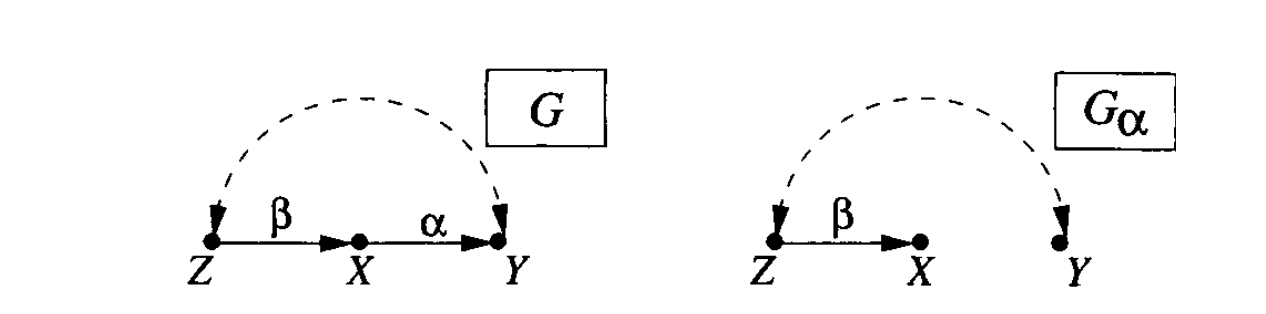
\includegraphics[scale=0.6]{imgs/img31.png}
	\end{center}
	\caption{$\alpha$ can be estimated as $r_{YX\cdot Z}$}
	\label{fig:path_coef_estimation}
\end{figure}

\begin{align}
	y = \alpha x + \beta_1z_1 + ... + \beta_kz_k + \varepsilon
\end{align}

Thus, we obtain the theorem

\begin{theorem}
	\textbf{Single-door criterion for direct effects} Let $G$ be any path diagram where $\alpha$ is the coefficient assigned to the edge $X \to Y$, and $G_\alpha$ is the diagram obtained by removing the edge $X\to Y$ from G. The coefficient $\alpha$ is identifiable if there exists a set $Z$:
	
	(i) $de(Y) \cap Z = \emptyset$
	
	(ii) $Z$ d-separates $X,Y$ in $G_\alpha$
	
	In this case $\alpha = r_{YX\cdot Z}$
	
	Conversely, if $Z$ does not satisfy these conditions, then $r_{YX\cdot Z}$ is not a consistent estimator of $\alpha$.
\end{theorem}

It may happen that the direct effect of $X$ on $Y$ cannot be estimated, as in the case of the diagram \ref{fig:total_effect}. However, it may still be possible to estimate the total effect. To identify it, it is necessary to choose a set $Z$ such that no paths other than directed $X \leadsto Y$ contribute to $r_{YX\cdot Z}$, that is, are blocked by $Z$.

Accordingly, we have the theorem 

\begin{theorem}
	For any two variables $X,Y$, the total causal effect of $X$ on $Y$ is identifiable if 
	
	(i) $Z \cap de(X) = \emptyset$
	
	(ii) $Z$ d-separates $X,Y$ in $G_{\underline X}$, that is, blocks all backdoor paths from $X$ to $Y$
	
	If these two conditions are met, then the total effect is estimated as $r_{YX \cdot Z}$
\end{theorem}

\begin{figure}[h]
	\begin{center}
		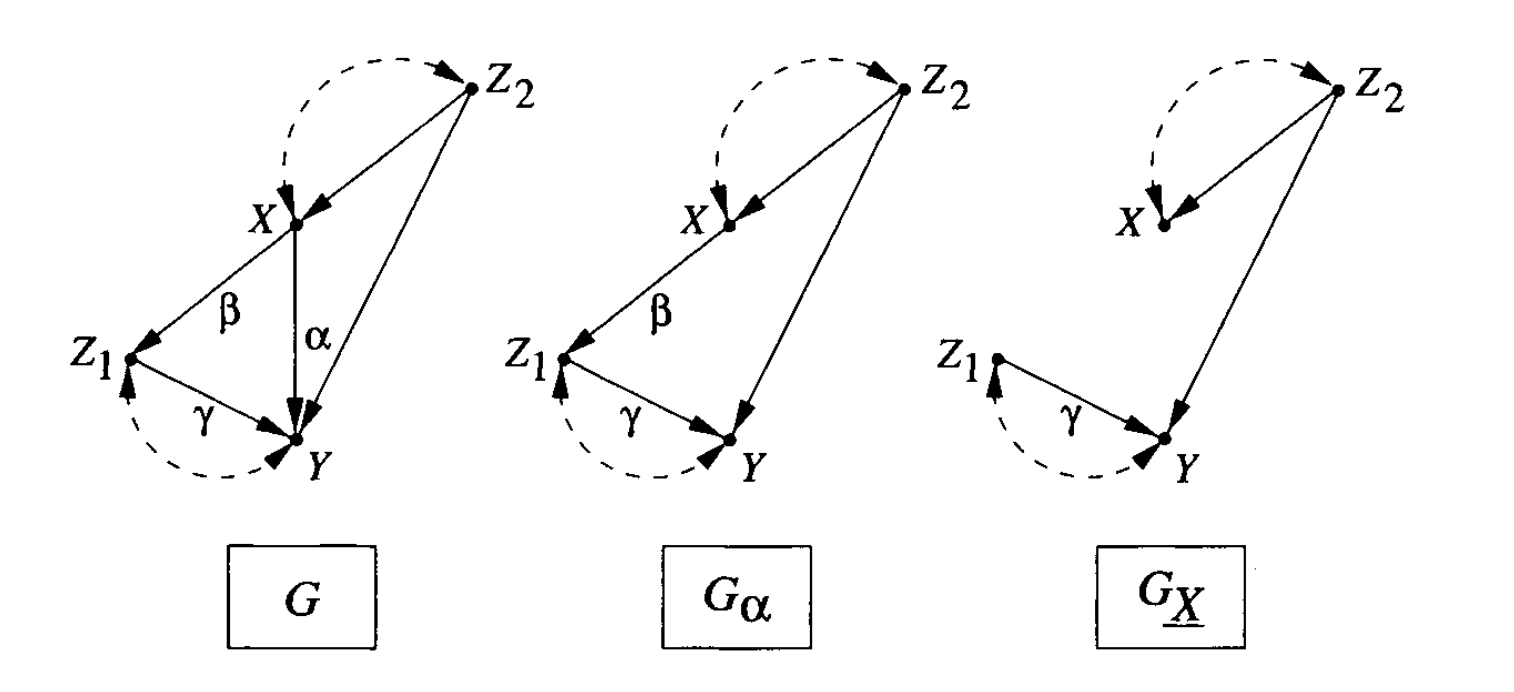
\includegraphics[scale=0.6]{imgs/img32.png}
	\end{center}
	\caption{$\alpha$ is not identifiable, but the total effect of $X$ on $Y$, equal to $\alpha + \beta \gamma $ can be estimated as $r_{YX|\cdot Z_2}$}
	\label{fig:total_effect}
\end{figure}


By analogy with these two extreme cases - total effect and direct effect - in general, we can introduce the concept of a partial effect, which is defined as the part of the effect of $X$ on $Y$ acting through some subset of directed paths. It can be computed by analogy by blocking all other paths (directed and non-directed) with some set $Z$. 

Interestingly, sometimes the total effect is not definable by itself but requires defining each component that constitutes it separately. In general, this is logical, since the previous theorem does not claim that this is a \textit{necessary} criterion for the identifiability of the total effect - which is logical, since we have previously learned to identify effects not only by the backdoor criterion.

For example, in the case of \ref{fig:path_coef_estimation}, we cannot, using the last theorem, estimate the effect of $Z$ on $Y$, since we cannot block the backdoor path $Z \leadsto Y$ in any way. However, we can estimate the total effect of $Z$ on $X$: $\beta = r_{XZ}$, and we can estimate the total effect of $X$ on $Y$ - $\alpha = r_{YX\cdot Z}$, from which we can express the total effect of $Z$ on $Y$ equal to $\alpha\beta$.

\begin{figure}[h]
	\begin{center}
		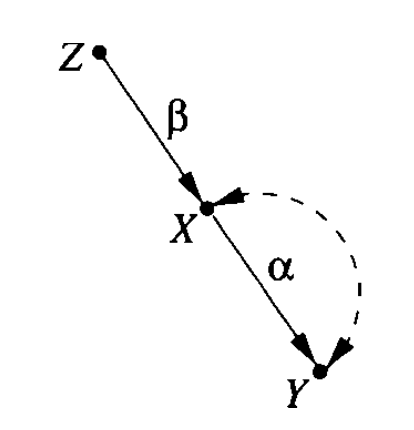
\includegraphics[scale=0.6]{imgs/img33.png}
	\end{center}
	\caption{$\alpha$ is determined using an instrumental variable $Z$}
	\label{fig:path_coef}
\end{figure}


Another example where we need to be clever is in the picture \ref{fig:path_coef}, where $\alpha$ cannot be estimated directly, but we can estimate the effect of $Z$ on $X$: $\beta = r_{XZ}$, and the effect of $Z$ on $Y$: $\alpha \beta = r_{YZ}$, from which $\alpha = \frac{r_{YZ}}{r_{XZ}}$

\subsubsection*{Comparison with the Nonparametric Approach}

The power of parametric methods is of course greater than that of nonparametric ones: thus, usually in the nonparametric case identification is possible, while in the parametric case it is not possible to precisely determine the type of functional dependence.

However, identification is not an end in itself, and sometimes it is not necessary. For example, if we only need to solve prediction problems, without interventions, then in general everything necessary is encoded in the covariance matrix, and we generally do not care about the specific values of the functions $f_i$ that define the variables functionally.

Let us repeat again that the meaning of structural equations is that they describe the physical laws by which a particular variable is generated, and the equality in these models is not symmetric. To predict the effects of interventions, it is important that we have a correct model of data generation.

\subsection*{Some Conceptual Remarks}

\subsubsection*{What Do Structural Coefficients Really Mean?}

Consider the SEM $y = \beta x + \varepsilon$. If we interpret $\beta$ as the change in $E[Y]$ for a unit change in $X$, then there may be a temptation to write $x = \frac{y - \varepsilon}{\beta}$ and in turn interpret $\frac{1}{\beta}$ as how much $E[X]$ changes for a unit change in $Y$. But this conflicts with both intuition and the model's prediction: the change in $E[x]$ should be 0 when $Y$ changes if $Y$ is not an independent variable in the original, structural equation for $X$.

There are two approaches to dealing with this situation, but both are bad. The first is not to endow $\beta$ with any causal meaning at all, but only to say that $\beta$ is a measure of the reduction in the variance of $Y$ explainable by $X$, but this conflicts with the desire to use SEMs for policy selection and generally with intuition. The second approach is to impose on $\varepsilon$ the restriction that it is not correlated with $X$. Then it will be correlated with $Y$, and the symmetry disappears. But in this case, we face the problem that just as $Y$ can be defined in terms of $y = \beta x + \varepsilon_1$, symmetrically $x = \alpha y + \varepsilon_2$, $\alpha = \beta \frac{\sigma_X^2}{\sigma_Y^2}$, where $cov(x, \varepsilon_1) = cov(y, \varepsilon_2) = 0$, and then we are forced to endow both $\beta$ and $\alpha$ with causal meaning as they turn out to be equal - but this also does not fit with the intuition that $X$ should not respond to interventions in $Y$ if it was not in the structural equation for $X$.

So what then is the meaning of structural equations, the coefficient $\beta$, and the error term? The answer is given by the following definition:

\define{Operational Definition of SEM} The equation $y = \beta x + \varepsilon$ is called structural if it is interpreted as follows: in an ideal experiment where we set $X = x$, and any other variables $Z$ not containing $X,Y$ are set to some fixed value $z$, the value $y$ is determined according to the structural equation, with $\varepsilon$ not being a function of $x,z$.

Note that the operational definition does not assert anything about the behavior of $X$ when fixing $Y$: if we observe $X$ and $Y$, then there is symmetry: from observing $Y = 0$ we can conclude $X = -\frac{\varepsilon}{\beta}$, but when we have interventions, there is no longer symmetry - this is obvious when we look at the diagram corresponding to the equations, where the arrows explicitly allow us to set this asymmetry.

The strongest statement that follows from the SEM $y = \beta x + \varepsilon$ is that $Y$ is causally dependent \textit{only} on $X$, thus $P(y|do(x),do(z)) = P(y|do(x))$, that is, any interventions do not affect $Y$ if we control $X$.

\define{Operational Definition of Structural Parameters} The meaning of the coefficient $\beta$ is 

\begin{align}
	\beta = \frac{\partial }{\partial x}E[Y|do(x)]
\end{align}

In this interpretation, it does not matter whether $X,\varepsilon$ are correlated or not. It has already been discussed earlier that $\beta$ is generally not equal to the regression coefficient, and is not directly related to $E[Y|x]$.

Finally, the operational definition of noise is 

\begin{align}
	\varepsilon = y - \E[y|do(x)]
\end{align}

Thus, the noise can be estimated both from controlled data (if we conduct a series of experiments with $do(x)$ and record the data $Y$, and then compute the expectation as the sample mean), and from observed data by the formula $\varepsilon = y - \beta x$, if we know $\beta$, since $\beta$ does not change depending on whether we observe or intervene.

Similarly, we can estimate the covariances of the noises for any two non-adjacent variables $X,Y$:

\begin{align}
	\E[\varepsilon_Y\varepsilon_X] = E[YX|do(pa_X),do(pa_Y)] - E[X|do(pa_X)]E[y|do(pa_Y)]
\end{align}

Again, if we have already established the model coefficients, then on the right we will have known linear functions, and everything can be calculated. If not established - we conduct controlled experiments with fixing $PA_X,PA_Y$.

\section{Simpson's Paradox, Confounding, and Collapsibility}

\subsection*{Anatomy of Simpson's Paradox}

In this section, we will understand why the effect described by Simpson in 1951 (but first noticed by Pearson in 1899) is generally perceived as a paradox.

The paradox is as follows: let there be some event $C$ that increases the probability of event $E$ in the population, but at the same time decreases the probability of the event in each of two subpopulations $F$ and $\neg F$:

\begin{align}
	P(E|C) > P(E|\neg C) \label{eq:simpson1} \\
	P(E|C,F) < P(E|\neg C, F) \label{eq:simpson2} \\
	P(E|C,\neg F) < P(E| \neg C, \neg F) \label{eq:simpson3}
\end{align}

From the point of view of simple probability theory, there is nothing surprising in such a situation; it begins to seem paradoxical when we endow the probabilistic relations with an additional \textit{causal} meaning.

For example, if we take $C$ to be the taking of a certain drug, $E$ to be the outcome of treating a disease, and $F$ to be gender (female/male), then by giving causal meaning to the expressions, we can come to the conclusion that the drug is harmful for both women and men, but overall it is beneficial.

What's the matter? The fact is that $P(E|C)$ should not be perceived as the effect of treatment: this is what we passively observe in the sample; the effect of treatment (from the action performed by the doctor) is expressed as $P(E|do(C))$. $P(E|C) > P(E|\neg C)$, in turn, is just some confirmation that $C$ can positively influence recovery - either due to a causal effect or due to random confounding through common causes.

\begin{figure}[h]
	\begin{center}
		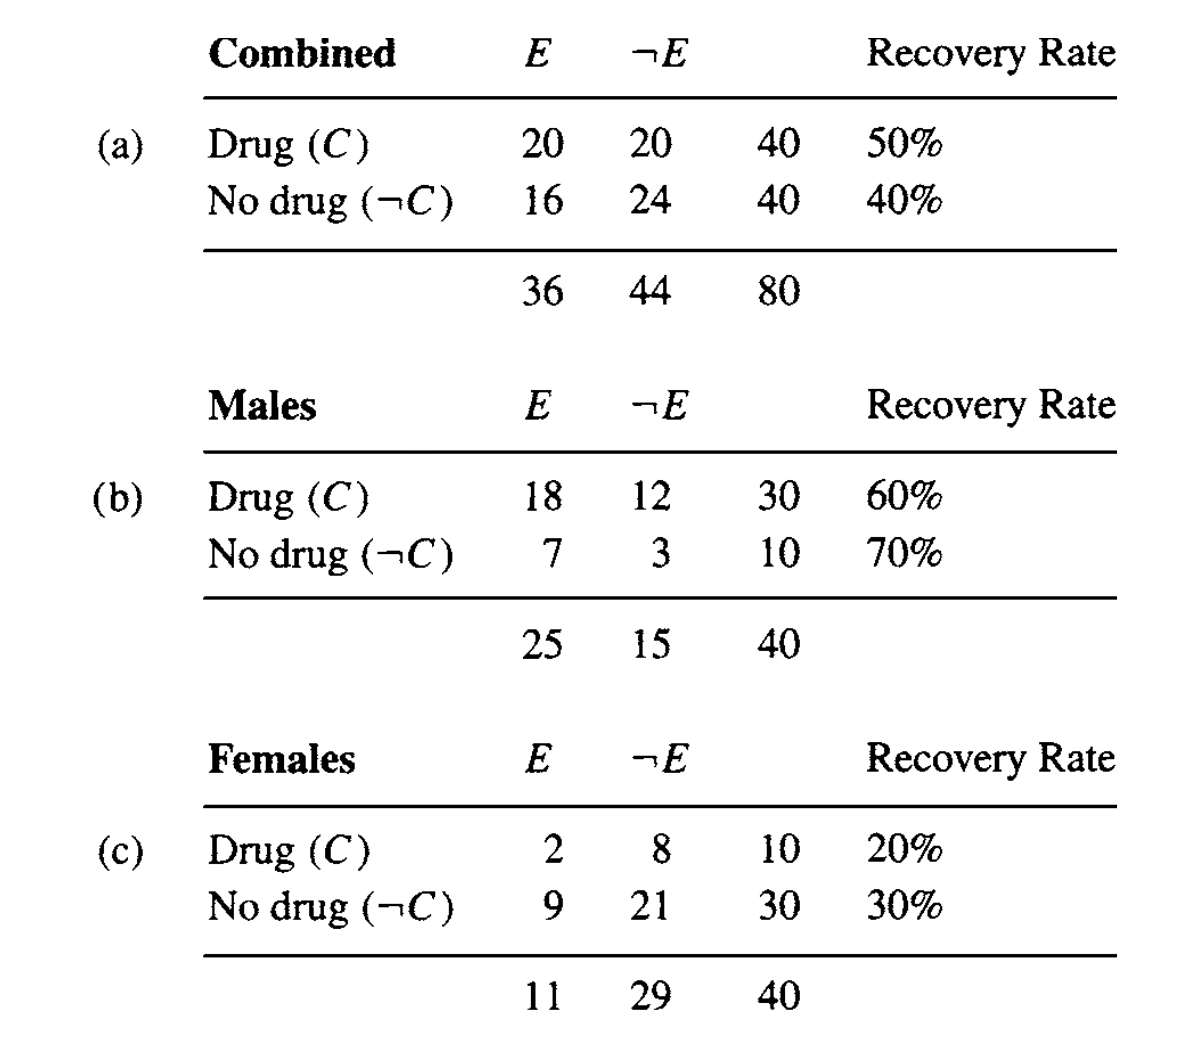
\includegraphics[scale=0.5]{imgs/img28.png}
	\end{center}
	\caption{Example data for Simpson's paradox}
	\label{fig:simpson}
\end{figure}


In this case, if we assume that gender is a common cause for taking the drug and for recovery, the effect of the drug should be estimated weighted for men and women. Thus, if gender $F$ is the only confounding factor, then \ref{eq:simpson2}, \ref{eq:simpson3} correctly reflect the effectiveness of the drug in the respective subpopulations, and \ref{eq:simpson1} denotes its evidential weight in the absence of information about gender (roughly speaking).

In the statistical literature, the paradox was not particularly linked to causality, because it was perceived as a purely imaginary construct.

What is characteristic is that throughout the existence of the paradox, statisticians did not really understand why the reversal of inequality signs causes such cognitive dissonance in people: after all, there seems to be nothing unnatural in the fact that probabilities behave this way and not otherwise when conditioned.

In 1981, Lindlie and Novick were the first to show the non-statistical nature of Simpson's paradox. Following the traditions of Bayesian decision theory, they decided to answer a practical question: a new patient arrives - should we use the drug or not? The immediate answer "If we know the patient's gender - then the drug should not be given, and if we do not know - then the drug should be given" - sounds strange and is certainly not correct in essence.

The next step the guys asked themselves - are there any additional statistical data that could incline us in favor of a separate or joint table for decision making. They answered this question negatively: with the same data, depending on the semantics, it may turn out to be correct to choose either one table or the other: so, if the semantics of $F$ was that it is gender - then we must make a decision according to statistics conditioned on gender. If $F$ is blood pressure, as in the picture \ref{fig:simpson2} (b), which is affected by the drug, and it affects recovery, then of course we should focus on data not conditioned on $F$ - and conditioning on the consequence $C$ will be incorrect, since we will thereby block one of the two causal paths.

\begin{figure}[h]
	\begin{center}
		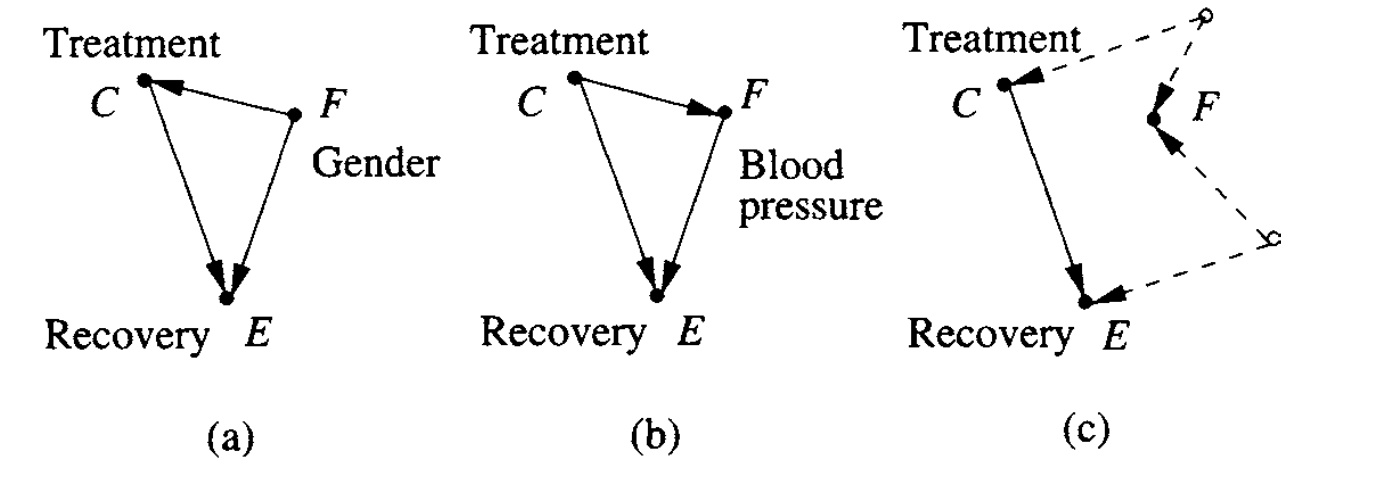
\includegraphics[scale=0.6]{imgs/img29.png}
	\end{center}
	\caption{The choice of which data to base the decision on - conditioned on $F$ or not - depends on the underlying causal structure}
	\label{fig:simpson2}
\end{figure}

What is the cause of the paradox? In general, a paradox arises when our set of implicit existing assumptions turns out to be in conflict with each other. In the case of Simpson's paradox, we have two competing beliefs

1. The assumption that causal relationships are governed by probability calculus

2. A set of implicit assumptions that describe our causal intuition

The first assumption is confirmed by explicit examples of data where inequalities \ref{eq:simpson1}-\ref{eq:simpson3} turn out to be consistent. The second says that there is no magic drug that is harmful for both men and women - but beneficial for a person in general, if we do not know their gender.

To resolve the paradox, we must either abandon causal intuition or the assumption that causal connections are governed by the laws of standard probability calculus. Of course, we will choose the second option - causality operates according to its own laws and requires an extension of probability calculus for its correct description.

For this, we will use the mechanics of do-calculus. Let us show that if 

\begin{align}
	P(E| do(C), F) < P(E|do(\neg C), F) \label{eq:simpson4}\\
	P(E| do(C), \neg F) < P(E|do(\neg C), \neg F)\label{eq:simpson5}
\end{align} 

then it cannot be that $P(E| do(C)) > P(E| do(\neg C))$, if $F$ is gender.

To do this, we prove the theorem 
\begin{theorem}
	If action $C$ reduces the probability of event $E$ in any subpopulation, then it must reduce the probability of event $E$ in the population as a whole, provided that the action does not change the distribution of subpopulations.
\end{theorem}

Let us prove for the particular case when there are only two subpopulations. So, let \ref{eq:simpson4} and \ref{eq:simpson5}. Since the action does not affect the distribution of subpopulations, then 

\begin{align}
	P(F|do(C)) = P(F|do(\neg C)) = P(F)
\end{align}

Let us decompose $P(E|do(C))$ by subpopulations:

\begin{align}
	\begin{split}
		P(E|do(C)) &= P(E|do(C),F)P(F|do(C)) + P(E|do(C),\neg F)P(\neg F| do(C)) \\
		&= P(E|do(C),F)P(F) + P(E|do(C),\neg F)P(\neg F)
	\end{split}
\end{align}

Similarly, let us decompose for $P(E|do(\neg C))$:

\begin{align}
	P(E|do(\neg C)) = P(E|do(\neg C),F)P(F) + P(E|do(\neg C),\neg F)P(\neg F)
\end{align}

Since both factors in the first equation are less than both factors in the second, the sum in the first case will ultimately be less than in the second.

$\blacksquare$

Our causal intuition arises from the obvious assumption that the drug cannot affect gender. At the same time, when $F$ is pressure, we can no longer be sure that the drug does not affect it.

\subsection*{Confounding}

In terms of meaning, confounding from the point of view of statistics is a situation where the association between two variables is present not only due to the effect by which one variable affects the other, but also due to the presence of some common causes. Thus, conceptually, the association between $X$ and $Y$ is confounded if there is a third variable $Z$ that affects both $X$ and $Y$.

It sounds simple, but in practice it has not been possible for a long time to transfer this concept to a mathematical language: it was not clear how to formalize the \textit{effect} of a variable on another.

There is an empirical description of the effect as an association that will \textit{prevail} in the case of a controlled randomized experiment - but such a description cannot be transferred to the language of probability theory, because this theory implies static conditions of application, and does not allow predicting which relations will dominate under \textit{changes} of these conditions.

It is precisely for the mathematical description of effects that the do-operator we use was primarily developed, thanks to which it is possible to express the effect in the form $P(y|do(x))$.

Despite the difficulties, statisticians, economists, and epidemiologists have long tried to develop formal criteria for the presence of confounding, and below we will consider why they are bad and how they can be fixed.

Let's start with the causal definition of confounding:

\define{Unconfoundedness (causal definition)} Let $M$ be a causal model of the data-generating process. Denote by $P(y|do(x))$ the probability $Y = y$ when performing the intervention $X=x$. We say that $X, Y$ are unconfounded in $M$ if 
\begin{align}
	P(y|do(x)) = P(y|x)
\end{align}
for any $x,y$ in their domain, where $P(y|x)$ is the conditional distribution generated by $M$.

This is the definition we will use to describe unconfoundedness. When there is no confounding between $X$ and $Y$, we say that $P(y|x)$ is an unbiased estimate of the effect.

\define{Unconfoundedness (associational definition)} Let $T$ be a set of variables that are \textit{not affected} by $X$. We will say that $X$ and $Y$ are unconfounded in the presence of $T$ if $\forall Z \in T$ at least one of the two holds:

(U1) $Z$ is not associated with $X$: $P(x|z) = P(x)$

(U2) $Z$ is not associated with $Y$ when conditioning on $X$: $P(y|z,x) = P(y|x)$.


Note that even such a seemingly purely statistical definition nevertheless contains a mysterious concept from the point of view of probability theory \textit{influence of one variable on another}. In fact, this is a causal concept, but it is indispensable in the study of effects, so everywhere further in the statistical approach to confounding we will nevertheless assume that the researcher somehow knows which variables affect which.

\subsection*{When the Associational Criterion for Confounding Fails}

\subsubsection*{Failure of Sufficiency of the Associational Criterion}

Consider this example: $Z_1, Z_2$ - the outcome of tossing two fair coins. $X = Z_1 == Z_2$, $Y = Z_1 != Z_2$. It is clear that individually $Z_1$, $Z_2$ do not confound $X,Y$: $P(x|z_1) = P(x|z_2) = 0.5 \forall x, z_1, z_2$, that is, $U_1$ holds. However, the pair $(Z_1,Z_2)$ confounds $X,Y$: despite the absence of a causal connection, they turn out to be negatively correlated in such a context.

Another problem with the associational definition is that we need to enumerate \textit{all} variables that are not affected by $X$. If we do not measure some, then we may conclude that there is no confounding when there is - and generally speaking there is no way to check that we have taken into account all variables.

\subsubsection*{Failure of Necessity of the Associational Criterion}

It is not difficult to give an example where a variable $Z$ fails both conditions $U1, U2$ but at the same time there is no confounding between $X,Y$. For example, consider \ref{fig:confounding}.

\begin{figure}[h]
	\begin{center}
		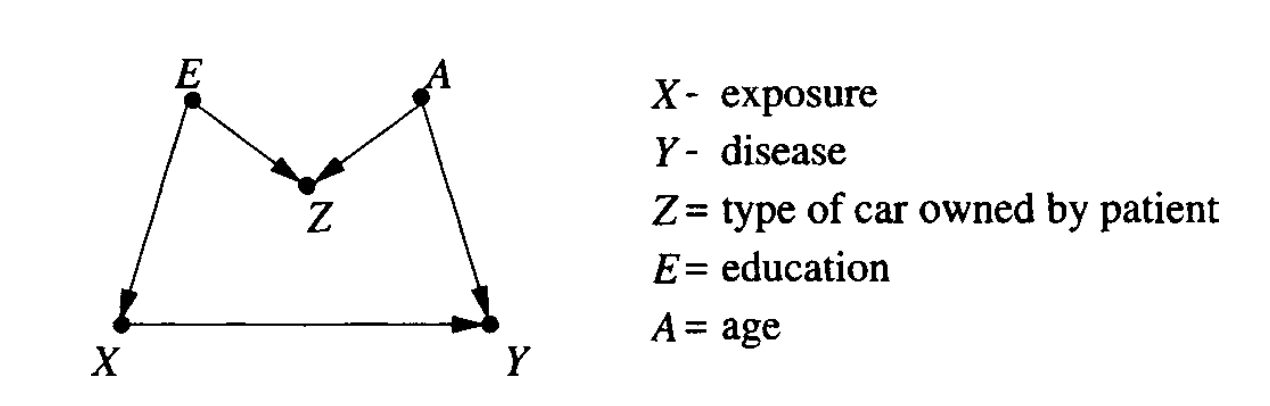
\includegraphics[scale=0.6]{imgs/img30.png}
	\end{center}
	\caption{Variable $Z$ fails both conditions of the associational criterion for unconfoundedness, but does not lead to confounding}
	\label{fig:confounding}
\end{figure}

\subsection*{Stable and Unstable Unbiasedness}

\define{Stable unbiasedness} Let $A$ be a set of assumptions/constraints imposed on the data-generating process, $C_A$ - the class of causal models satisfying $A$. An estimate of the effect of $X$ on $Y$ is stably unbiased if $P(y|do(x)) = P(y|x)$ holds $\forall M \in C_A$. Accordingly, a pair of variables $X,Y$ is called stably unconfounded.

Assumptions that usually limit the class of considered causal models are represented either parametrically or topologically. For example, in the case of models defined by structural equations, the constraints may consist in the fact that we consider only linear models with normal noise.

Weaker constraints are imposed by the topological structure of the causal diagram - here we do not specify noise distributions and the functional form of the relationship between variables. Let us consider the statistical consequences of such nonparametric constraints.

As we know, when the diagram is acyclic, the backdoor criterion gives a necessary and sufficient test for unconfoundedness. Thus, we obtain the theorem

\begin{theorem}
	\textbf{Common Cause Principle} Let $A_D$ be the set of constraints defined by an acyclic causal diagram $D$. Variables $X,Y$ are stably unconfounded given $A_D$ if and only if $X, Y$ have no common ancestor in $D$.
\end{theorem}

If there is no common ancestor ($\Leftarrow$), then there is no confounding by the backdoor criterion. That there is no ancestor if there is no confounding ($\implies$) is proved by providing a specific example of a distribution that violates this condition (it seems this is not difficult).

$\blacksquare$

Suppose, however, that we do not have a causal diagram at hand. Suppose all we know about any variable $Z$ is whether it definitely has no effect on $Y$, and whether $X$ has an effect on it. The question is - will such, reduced information be enough to detect the presence or absence of confounding?

\begin{theorem}
	\textbf{Criterion for Stable Absence of Confounding} Let $A_Z$ be assumptions consisting in that the data is generated by
	
	(i) an acyclic (though unknown) model M
	
	(ii) $Z$ is a variable in $M$ that is not affected by $X$ (no directed path $X \leadsto Z$) and possibly affects $Y$ (this means that in the underlying diagram there is a directed path $Z \leadsto Y$). 
	
	Then, if both conditions U1, U2 of the associational definition of confounding are failed, that is, if (U1) $X \not \independent Z$ and (U2) $Z \not \independent Y | X$, then $X, Y$ are stably confounded.
\end{theorem}

Indeed, by the previous theorem, if the variables are unconfounded, they have no common ancestor. But if they have no common ancestor, then either U1 or U2 must hold for any $Z$ satisfying $A_Z$.

$\blacksquare$

Thus, we have found a sufficient but not necessary statistical criterion for confounding.
	
\end{document}